\documentclass[10pt,letterpaper]{article}

%% -packages-
\usepackage{graphicx}
\usepackage{epstopdf}
\usepackage{psfrag}
\usepackage[round]{natbib}
\usepackage{longtable}
\usepackage{rotating}
\usepackage{rotate}
\usepackage{lscape}
\usepackage{amssymb}
\usepackage{amsmath}
\usepackage[colorlinks,bookmarks,citecolor=magenta]{hyperref}
\usepackage{color}
\usepackage{multicol}
\usepackage{alltt}
\usepackage{listings}


\lstset{ %
language=R,                % choose the language of the code
basicstyle=\footnotesize,       % the size of the fonts that are used for the code
numbers=left,                   % where to put the line-numbers
numberstyle=\footnotesize,      % the size of the fonts that are used for the line-numbers
stepnumber=2,                   % the step between two line-numbers. If it's 1 each line 
                                % will be numbered
numbersep=5pt,                  % how far the line-numbers are from the code
backgroundcolor=\color{white},  % choose the background color. You must add \usepackage{color}
showspaces=false,               % show spaces adding particular underscores
showstringspaces=false,         % underline spaces within strings
showtabs=false,                 % show tabs within strings adding particular underscores
frame=single,                   % adds a frame around the code
tabsize=2,                      % sets default tabsize to 2 spaces
captionpos=b,                   % sets the caption-position to bottom
breaklines=true,                % sets automatic line breaking
breakatwhitespace=false,        % sets if automatic breaks should only happen at whitespace
title=\lstname,                 % show the filename of files included with \lstinputlisting;
                                % also try caption instead of title
escapeinside={\%*}{*)},         % if you want to add a comment within your code
morekeywords={*,...}            % if you want to add more keywords to the set
}



%\usepackage[latin1]{inputenc} % To use characters such as � without typing \'e
%\usepackage[cyr]{aeguill} % To display characters such as �
%\usepackage{xspace} % To get the right spacings in front of : and so on
\usepackage[french,english]{babel}

%% ---------------------------------------------------------------------
%%Page Layout Properties-------------------------------------------------

%\voffset 0in \textwidth 7.0in  \oddsidemargin 0in
%\evensidemargin 0in \headheight 0.in \textheight 9in  %%Look at Box13.1 for text scale
\voffset -0.75in
\hoffset -0.75in
\textwidth 6.5in%
\textheight 8.5in%
%\evensidemargin 0.in%

%\textwidth 6in%
%\topmargin 0in%
\setlength{\LTcapwidth}{\textwidth} %caption width for longtables

%Arial font
\renewcommand{\rmdefault}{ppl} % Arial
\renewcommand{\sfdefault}{ppl} % Arial phv  % palatino ppl

	
	
%Logo
\usepackage{fancyhdr}
\renewcommand{\headheight}{0.6in}
\setlength{\headwidth}{\textwidth}
\fancyhead[L]{}% empty left
\fancyhead[R]{ % right
   \includegraphics[height=0.53in]{iscamlogo.eps}
}
\pagestyle{fancy}

% %Logo
% \usepackage{fancyhdr}
% \renewcommand{\headheight}{0.6in}
% \setlength{\headwidth}{\textwidth}
% \fancyhead[L]{}% empty left
% \fancyhead[R]{ % right
%    \includegraphics[height=0.53in]{iscamlogo.eps}
% }
% \pagestyle{fancy}


%-------------------------------------------------------------------------
%Water mark
%%\usepackage{eso-pic}
%%\usepackage{graphicx}
%%\usepackage{color}
%%\usepackage{type1cm}
%%\usepackage{float} 
%%
%%\makeatletter
%%  \AddToShipoutPicture{%
%%    \setlength{\@tempdimb}{.5\paperwidth}%
%%    \setlength{\@tempdimc}{.5\paperheight}%
%%    \setlength{\unitlength}{1pt}%
%%    \put(\strip@pt\@tempdimb,\strip@pt\@tempdimc){%
%%      \makebox(0,0){\rotatebox{45}{\textcolor[gray]{0.85}{\fontsize{1.75cm}{1.75cm}\selectfont{DRAFT  \today}}}}
%%    }
%%} \makeatother


%% -math-
\newcounter{saveEq}
  \def\putEq{\setcounter{saveEq}{\value{equation}}}
  \def\getEq{\setcounter{equation}{\value{saveEq}}}
  \def\tableEq{ % equations in tables
    \putEq \setcounter{equation}{0}
    \renewcommand{\theequation}{T\arabic{table}.\arabic{equation}}
    \vspace{-5mm}
    }
  \def\normalEq{ % renew normal equations
    \getEq
    \renewcommand{\theequation}{\arabic{section}.\arabic{equation}}}

  \def\puthrule{ %thick rule lines for equation tables
    \hrule \hrule \hrule \hrule \hrule}


%%\newcommand{\msy}{$C^*$}
%%\newcommand{\fmsy}{$F^*$}
%%\newcommand{\sbmsy}{$\rm{SB_{MSY}}$}
%%\newcommand{\sbfour}{$\rm{SB_{40}}$}
%%\newcommand{\�}{\'e}
%%\newcommand{\�}{\`e}
%%\newcommand{\�}{\`a}
%%\newcommand{\�}{\^e}
%\newcommand{\iscam}{
%{$^i$}\textcolor{red}{S}\textcolor{green}{\small{}C}{\textcolor{blue}{\footnotesize{}A%}}\textcolor{black}{$_\textnormal{M}$}}%{\raisebox{-0.7ex}{M}}%

%\input logo.sty


\newcommand{\fmsy}{F$_{\textnormal{MSY}}$}
\newcommand{\bmsy}{B$_{\textnormal{MSY}}$}

%% ---------------------------------------------------------------------


\makeatletter
\newenvironment{tablehere}
  {\def\@captype{table}}
  {}

\newenvironment{figurehere}
  {\def\@captype{figure}}
  {}
\makeatother

%iscam logo
\newcommand{\iscam}{
	\raisebox{0.75ex}{$i$}%
	\textcolor{red}{\raisebox{0.25ex}{S}}%
	\textcolor{green}{\raisebox{0.00ex}{C}}%
	\textcolor{blue}{\raisebox{-.25ex}{A}}%
	\raisebox{-.50ex}{M}%
	}%


%% ---------------------------------------------------------------------


\title{
\includegraphics[height=2.53in]{iscamlogo.eps}
\vfill
\iscam\ Users Guide\\
Version 1.0\\
\vfill}
\author{Steven Martell\\
University of British Columbia\\
Fisheries Centre\\
2202 Main Mall\\
Vancouver, BC\\
V6T 1Z4\\
Canada\\ 
\texttt{s.martell@fisheries.ubc.ca}}
\date{\small{$^\copyright$  Copyright Steven Martell, \today.  All rights reserved.}}







\begin{document}

\pagenumbering{roman}
\setcounter{page}{1}
    \maketitle \thispagestyle{empty}
%    \vfill
%    \noindent\hrulefill\\
%    Draft document for peer review: Started on Wednesday, February 11, 2009\\
%    Draft document completed on Thursday, February 19, 2009\\
%    Final document completed on Wednesday, March 4, 2009.\\
%    CSAS revisions completed on Wednesday, March 11, 2009.
%    \clearpage
\thispagestyle{empty}
\clearpage


\newpage


%\begin{abstract}
%This is the abstract
%  \end{abstract}
%\clearpage


%%
 \selectlanguage{english}

    %\input{ToDoList}
%% -Executive summary material------------------------------------------

\pagenumbering{roman}
\section*{Preface}
\addcontentsline{toc}{subsection}{Preface}
This document is the users guide for the fisheries stock assessment model \iscam, or Integrated Statistical Catch Age model.  This assessment package was written by Steven Martell and may be freely used by others, but in no way am I responsible for the mess that may or may not happen if you use this software to do your job.  Although I try hard, I cannot guarantee that this application is 100\% free of bugs/coding errors so double check your own work and see if it makes sense.  If you find a bug, fix it, recompile the code and continue on.  Or let me know about the bug and I'll happily  fix it for you,  if I have time.


\section*{Acknowledgements}
\addcontentsline{toc}{subsection}{Preface}
I greatly appreciate the early feedback I received from Jake Schweigert (DFO Pacific Biological Satiation, Nanaimo, BC) while developing this software and the users guide.  Also feedback, error checking, and code from Vivian Haist, Jim Ianelli, Robyn Forrest and Chris Grandin.  Much of the linkage between ADMB and R was inspired by my DFO colleagues and friends, Rob Kronlund, Jon Schnute, and Jaclyn Cleary.


%%%!TEX root = /Users/stevenmartell/Documents/CURRENT PROJECTS/iSCAM-trunk/fba/BC-herring-2011/WRITEUP/BCHerring2011.tex


%\subsection*{Abstract}
%\addcontentsline{toc}{subsection}{Abstract}
%
%June 15, 2011.  Structure of this paper has changed a bit. This document will now consist of an assessment and forecast of the five major stocks and the two minor stocks.  There will be at least 5 appendixes that 1) describe the input data and the control files used for the assessment model, 2) a detailed description of \iscam, 3) a description of the methods used to develop the prior distribution, 4) simulation testing of the \iscam model, 5) moving toward the sustainable fisheries framework (see Cleary and Cox paper) and include discussion of the issues of developing an MSY-based framework for a multigear fishery with changing selectivities and natural mortality rates, and finally 6) a list of research recommendations.
%
%Summary:  Three major themes of the paper: 1) a comparing HCAM and iSCAM (where iSCAM is set up with nearly the same assumptions as 2010 HCAM assessment), 2) an iSCAM assessment with several scenarios addressing (a) q with various priors, (b) time-varying versus constant M, (c) alternative selectivity models, and (d) the interactions of all three of these confounded variables, and 3) an iSCAM assessment with the test fishery and seine roe fishery data separated into specific fleets.  The side by side comparison will examine similarities/differences between trends in biomass, fishing mortality rates, and residual fits to the spawn survey data an age-composition data.  These two models have some fundamental differences in the statistical assumptions about the catch-at-age data, so results are likely to be slightly different.  Results for all three themes will focus on reconstructing table 5 from last years assessment, with the addition of LRP and USRP to be compared with the cuttoffs and catch advice for low med and high recruitment.
%


\section*{Abstract}\addcontentsline{toc}{part}{Abstract}



\section*{Executive summary}


\newpage
\tableofcontents
\addcontentsline{toc}{subsection}{Contents}
\newpage
%% -Main body of the document-------------------------------------------
\pagenumbering{arabic}
	
%    cutoff%!TEX root = /Users/stevenmartell/Documents/CURRENT PROJECTS/iSCAM-trunk/fba/BC-herring-2011/WRITEUP/BCHerring2011.tex


\section{Introduction}

The objectives of this section of the report are: (1) present the data used in the 2011 assessment, (2) provide a summary overview of the integrated statistical catch-age model (hereafter, \iscam), (3) present the 2011 stock assessment and forecast for 2012, and (4) describe in detail the decision table used to provide advice to fisheries management.

BC herring are currently managed as five major stocks and 2 minor stocks (Figure \ref{Fig1}).  Annual catch advice for each of these areas is based on current estimates of stock status, and a 20\% exploitation rate if the post-fishery stock is above the cutoff level for the five major stocks and a 10\% exploitation rate for the two minor stocks.  Cutoff levels for the five major stocks historically were based on the 1996 estimate of  0.25$B_o$.  These cutoffs are currently thought to be more conservative 	than the suggested default Limit Reference Point of 0.4\bmsy\ \citep{dfo2006}. For example, \bmsy\ is normally in the range of 35\% of the unfished biomass for many fish stocks; therefore,  40\% of \bmsy is roughly 14\% of  unfished which is significantly lower than the 25\%$B_o$ that is currently used for Pacific herring.   Alternative cutoffs based on updated estimates of $B_o$ are also provided in this document.

This years assessment is based on a new model, \iscam, where alternative assumptions about survey $q$, and the form of the error distribution for the age-composition data are the major differences in comparison to the 2010 assessment using HCAM.  In addition to the changes in likelihoods, we also present an alternative parametrization of the gillnet selectivity to determine if the residual variation in gillnet age-composition data are better explained by systematic changes in the empirical weight-at-age data or selectivity has been relatively constant and natural mortality rates have varied over time.


In this part of the document, we first describe the five major and two minor Stock Assessment Regions (SARS) that comprise the BC herring stocks. We then present the input data used in this years assessment, briefly describe the analytical methods and diagnostics, describe the recruitment and catch forecasts, and the Harvest Control Rule (HCR) used for generating catch advice. We then present the maximum likelihood estimates of residual patterns and overall fits to the observations, summarize MSY based reference points and maximum likelihood estimates of \bo. Lastly, we present the results of integrating the joint posterior distribution, diagnostics for ensuring convergence, marginal parameter distributions (with prior distributions overlaid), and catch advice based on the median values of the joint posterior distribution.  The last section presents the data, MLE results, marginal distributions and catch advice for the two minor areas (the HCR in the minor area differs from the major areas).


\section{BC Herring Stocks}
The geographic boundaries used to delineate the B.C. herring stock assessment regions have remained consistent since 1993.  Boundaries and locations of the major stock and minor stock areas are identified in Figure \ref{Fig1}.  The Haida Gwaii (HG) or Queen Charlotte Islands (QCI2E) stock assessment region includes most of Statistical Area 2E, spanning from Cumshewa Inlet in the north to Louscoone Inlet in the south.  The Prince Rupert District (PRD) stock assessment region encompasses Statistical Areas 03 to 05.  The Central Coast (CC) assessment region separates the major migratory stocks from the minor spawning populations in the mainland inlets.  The Central Coast assessment region includes Statistical Area 07 plus Kitasu Bay in Area 06, Kwakshua Channel in Section 085 and Fitz Hugh Sound in Section 086.  The Strait of Georgia (SOG) stock assessment region includes all of Statistical Areas 14 to 19, 28, and 29 (excluding Section 293), Deepwater Bay and Okisollo Channel, both in Section 132, and Section 135.  The west coast of Vancouver Island (WCVI) assessment region encompasses Statistical Areas 23 to 25.  The minor stocks include all of Area 27 and Area 2W (excluding Louscoone Inlet in Section 006).  Current geographic stock boundaries are outlined in \cite{Midgley:2003fk}, although note that SOG sections 280 and 291 do not appear as they were added in 2006.

%%\begin{figure}[!tbp]
%%	% Requires \usepackage{graphicx}
%%	%\includegraphics[width=\textwidth]{Figs/HerringAreaMap.pdf}
%%	\includegraphics[width=0.95\textwidth]{../FIGS/PBSfigs/Assessment_Regions_2W_27_2010_HG.pdf}
%%	\caption{B.C. herring major stock areas: Haida Gwaii (HG or QCI 2E), Prince Rupert District (PRD), Central
%%Coast (CC), Strait of Georgia (SOG), West Coast Vancouver Island (WCVI), and minor stock areas: Area 2W and
%%Area 27.}\label{II:fig:map}
%%\end{figure}
    
\section{Running \iscam; input files \& command line options}
\begin{multicols}{2}


There are three required input files for \iscam: the \verb"iscam.dat" file, the \verb"datafile", and the \verb"controlfile".  By default when \iscam runs, the first file it looks for is the \verb"iscam.dat" file, unless otherwise specified by using the command line option \verb"-ind".  The following subsections explains the details of each of the data files.


%%%%%%%%%%%%%%%%%%%%%%%%%%%%%%%%%%%%%%%%%%%
\subsection{The \texttt{iscam.dat} file}
What is required in the \verb"iscam.dat" file is just the name of the data file and the control file, in that order.  An example is given below for the \texttt{PHake2010.dat} and \texttt{Phake2010.ctl} data and control files.
\begin{verbatim}
PHake2010.dat		#Data file name
PHake2010.ctl		#Control file name
\end{verbatim}
Note that it is necessary to have the \verb"*.dat", and \verb"*.ctl" extensions, as \iscam\ will read in the entire filename including the extension.  Also note that the \verb"#" symbol acts as a comment line, and \iscam\ will ignore the contents of the remaining line when reading in data.

%%%%%%%%%%%%%%%%%%%%%%%%%%%%%%%%%%%%%%%%%%%
\subsection{The data file}
The data file is composed of several required sections (required in the sense that they must be defined, but do not necessarily have to have data).  The first of these sections is the model dimensions.  Below is an example where the model starts in 1977 and the last year is 2009, the youngest age-group is 1 years old, and the oldest age-group is 15 years old and older (i.e., a plus group).  The total number of unique gears (including gear that samples fish in surveys is two, and last line is an integer vector that specifies if the gear is a fishery, or a survey (using 1 or 0, respectively).  For each gear you must specify 1 (a commercial fishery) or 0 (a fisheries independent survey).  Again the \verb"#" is a comment character and \iscam\ will ignore the contents after this character.  The following is an example of the model dimensions section:
\begin{verbatim}
##________________________
##____Model Dimensions____
1977		#first year of data
2009		#last year of data
1			#age of youngest age class
15			#age of plus group
2			#number of gears (ngear)
## flags for gears 
## fishery (1) or 
## survey (0) in ngears
1	0
##________________________
\end{verbatim}

The next required section is the age-schedule information pertaining to natural mortality, growth and maturity-at-age. For now, natural mortality is assumed to be age-independent.
\begin{verbatim}
## ________________________
## ___Age-schedules info___
#natural mortality rate (m)
0.23
#growth parameters (linf,k,to)
52, 0.32, 0
#length-weight allometry (a,b)
5e-6, 3.0
#maturity at age (am=log(3)/k) 
#& gm=std for logistic
3.45, 0.35
## ________________________
\end{verbatim}

Next is the time series data for the historical catch by year, fishery(ies) and survey(s).  Note that it is assumed that catch exists for each year that is specified in the model dimensions section (e.g., 1977-2009).  The first column is the year of the catch, and the subsequent columns are catch (in weight) for each fishery or survey.  Years where there are no catches (or no fishery) should be replaced by a 0.  In cases where surveys did not exist, or there were no removals (e.g., an acoustic survey), specify a zero catch for each year (row).  
\begin{verbatim}
## ________________________
#Time series data
#Observed catch 
#(1977-2009, 1,000,000 metric t)
#yr	commercial survey
1977 0.132693 0
1978 0.103639 0
1979 0.137115 0
...  omitted data for space
2008 0.321546 0
2009 0.176671 0
## ________________________
\end{verbatim}

The next section pertains to the relative abundance index, where first the number (\texttt{nit}) specified the number of independent surveys, and the next row specifies the number of observations (\texttt{nit\_nobs} ,or rows of data for each survey).  The first column is an integer vector that is used to index the survey year, the second column is the actual survey abundance index, and the third column is the gear index associated with this gear.  The fourth column is the relative weight that should be used for the index.  For example, setting wt=0 for a given year will result in omitting the data, or setting wt=2 would imply that the CV is one half of the other values.  The last column specifies the fraction of total mortality that has occurred when the survey was conducted (e.g., if the survey is conducted half way through the year then 0.5 implies that 1/2 of $Z_{t,a}$ has occurred when the survey was conducted).
\begin{verbatim}
## ________________________
#Relative Abundance index from 
#independent survey (it) 1970-2008
#nit
1
#nit_nobs
13
#iyr    it gear wt survey timing
1977 1.915  2  1   0.5
1980 2.115  2  1   0.5
1983 1.647  2  1   0.5
1986 2.857  2  1   0.5
...omitted data for space
2007 0.879  2  2   0.5
2009 1.460  2  0   0.5
## ________________________
\end{verbatim}

For age-composition information, a 3 dimensional array is used to store the information by gear-type (matrix), by year (rows of each matrix) and by age (columns of each matrix).  An example of the age composition data is shown on the following page.  

First you must specify the number of gears for which age-composition data exists.  If there are no data, then set this to 0. On  the next line you must specify the number of years of age-composition data there are for each gear type.  Next, for each gear, you must specify the first age-class of the data, and on the next row specify the oldest age-class of the data.  On the example in the next page, there are two gears, the first gear has 33 years of observations, and the second gear has 13 years of observations.  Each gear has the youngest age-class at 2 years and the oldest age-class at 15 years.  This means there are 14 columns of age-compositions for each gear type.  

The first two columns of the age-composition data refer to the year and gear type from which the data were obtained.  So in the example on the next page, the first 33 rows of the matrix (some of which is missing so it could fit on the page) corresponds to the years 1977-2009 for gear type 1, and from 1977 to 2009 every 2-3 years for gear type 2.  

The last component of the data file is an end of file ``eof'' marker, which is set to 999.  This is the last number read in from the datafile and \iscam\ checks to ensure it is 999.  If there is an error reading the datafile, \iscam\ will break and report that there was an error reading the data.


\begin{verbatim}
## ________________________
#eof
999
## ________________________
\end{verbatim}

\end{multicols}
%\begin{minipage}[b]{\linewidth}
%\centering
\begin{landscape}
\begin{footnotesize}
\begin{verbatim}
#Age composition data by year, gear (ages 2-15+)
#na_gears
2
#na_nobs
33	13
#a_sage
2	2
#a_page
15	15
#yr 	gear       V1       V2       V3       V4       V5       V6       V7       V8       V9      V10      V11      V12      V13      V14
1977    1 0.091087 0.039290 0.208628 0.028500 0.053160 0.211179 0.078270 0.079949 0.063640 0.058483 0.043761 0.029639 0.007592 0.006823
1978    1 0.022968 0.101932 0.068633 0.199094 0.033354 0.071961 0.208406 0.084622 0.072156 0.073040 0.024682 0.021006 0.013116 0.005030
1979    1 0.049457 0.089640 0.100254 0.046571 0.191908 0.071243 0.159754 0.158389 0.056370 0.037676 0.016184 0.010295 0.006469 0.005789
1980    1 0.009331 0.254593 0.042151 0.054263 0.050507 0.143816 0.065236 0.087843 0.169471 0.046122 0.037636 0.023076 0.008874 0.007079
1981    1 0.091224 0.062768 0.280898 0.012851 0.045430 0.047641 0.148751 0.062707 0.066417 0.125977 0.031183 0.012419 0.009671 0.002062
1982    1 0.181412 0.025886 0.016978 0.318964 0.032603 0.045648 0.045099 0.131034 0.027439 0.033879 0.119575 0.010972 0.006862 0.003648
1983    1 0.000322 0.327381 0.030386 0.021774 0.318861 0.034486 0.037515 0.044368 0.095257 0.024331 0.017871 0.037722 0.007340 0.002385
1984    1 0.000000 0.010415 0.546489 0.035445 0.072340 0.185115 0.023775 0.020842 0.014283 0.045333 0.009533 0.007920 0.024390 0.004121
1985    1 0.006798 0.006334 0.065169 0.607023 0.070421 0.058060 0.132423 0.011557 0.006879 0.007111 0.013539 0.002836 0.000000 0.011849
1986    1 0.111570 0.031159 0.007757 0.034088 0.485333 0.058011 0.043959 0.122124 0.022909 0.026576 0.014536 0.026627 0.004392 0.010957
1987    1 0.000000 0.264654 0.016305 0.003861 0.017893 0.540852 0.032262 0.016639 0.080708 0.003902 0.001822 0.005542 0.009811 0.005748
1988    1 0.002907 0.002881 0.325484 0.012085 0.007047 0.010794 0.464716 0.021331 0.009870 0.101698 0.001949 0.004157 0.001274 0.033806
1989    1 0.026833 0.022546 0.009612 0.452262 0.010250 0.004556 0.006132 0.394579 0.015267 0.006758 0.044542 0.000903 0.001179 0.004583
1990    1 0.048604 0.255566 0.024077 0.002273 0.251121 0.006576 0.001663 0.000990 0.323920 0.003924 0.000212 0.072414 0.000146 0.008513
1991    1 0.034754 0.176910 0.169392 0.027073 0.007271 0.316749 0.012094 0.001274 0.001349 0.206127 0.003853 0.000000 0.036791 0.006363
1992    1 0.035191 0.044184 0.126581 0.177710 0.021788 0.007533 0.344623 0.006212 0.001264 0.003920 0.198907 0.004982 0.000449 0.026655
1993    1 0.007327 0.219650 0.032109 0.141618 0.169717 0.014288 0.007544 0.287667 0.008052 0.001062 0.000425 0.104591 0.000492 0.005457
1994    1 0.000419 0.033794 0.194593 0.013819 0.121828 0.200067 0.013059 0.004773 0.307047 0.002355 0.004118 0.000280 0.096116 0.007732
1995    1 0.015172 0.001676 0.067824 0.247580 0.011946 0.076025 0.204514 0.017753 0.003065 0.259156 0.002369 0.003815 0.000000 0.089107
...	some missing data removed here to fit on page.
2005    1 0.008720 0.004799 0.070427 0.055023 0.684012 0.084118 0.021823 0.028355 0.019809 0.010432 0.008069 0.002582 0.000360 0.001470
2006    1 0.016047 0.109332 0.016100 0.086023 0.047267 0.606611 0.050565 0.017944 0.019738 0.012433 0.009263 0.004693 0.001532 0.002454
2007    1 0.135250 0.030604 0.145496 0.015585 0.070675 0.041936 0.441809 0.059055 0.018388 0.018549 0.012342 0.004254 0.004551 0.001507
2008    1 0.086419 0.307710 0.023174 0.134343 0.009449 0.035456 0.033322 0.305151 0.032058 0.010867 0.008882 0.005414 0.003330 0.004426
2009    1 0.007237 0.201241 0.298293 0.044466 0.140682 0.014182 0.025967 0.022153 0.193496 0.036166 0.005012 0.004290 0.003855 0.002961
1977    2 0.054308 0.051673 0.322415 0.029524 0.041387 0.358094 0.049372 0.036486 0.020920 0.019594 0.010201 0.003792 0.000997 0.001237
1980    2 0.004557 0.555127 0.053761 0.032569 0.026590 0.117668 0.043603 0.093838 0.037630 0.022180 0.003734 0.006424 0.001338 0.000983
1983    2 0.000265 0.785009 0.026011 0.007869 0.103384 0.016545 0.011402 0.008131 0.022356 0.005273 0.006223 0.006489 0.001042 0.000000
1986    2 0.604601 0.015879 0.002792 0.019748 0.266035 0.028628 0.022778 0.029920 0.003627 0.003812 0.000276 0.001440 0.000463 0.000000
1989    2 0.169990 0.058515 0.012874 0.526835 0.011735 0.004161 0.007554 0.179632 0.009473 0.000722 0.017782 0.000000 0.000000 0.000726
1992    2 0.089253 0.011915 0.069071 0.176823 0.021856 0.008862 0.432238 0.013086 0.007872 0.003964 0.149487 0.007606 0.000000 0.007967
1995    2 0.324964 0.043475 0.012039 0.212541 0.009810 0.032765 0.148871 0.002177 0.000000 0.158452 0.000354 0.006429 0.000000 0.048122
1998    2 0.168351 0.187074 0.157169 0.195749 0.014026 0.055093 0.087607 0.010731 0.015903 0.048868 0.003121 0.001999 0.042448 0.011861
2001    2 0.709921 0.089531 0.052761 0.056572 0.026180 0.026069 0.014190 0.008255 0.005804 0.002446 0.002162 0.004212 0.000400 0.001496
2003    2 0.029781 0.025334 0.640666 0.109500 0.027623 0.060058 0.039723 0.021949 0.022287 0.007181 0.004232 0.004367 0.003083 0.004214
2005    2 0.239916 0.024324 0.072095 0.051813 0.482518 0.052666 0.017966 0.024352 0.013884 0.011229 0.004744 0.002436 0.000323 0.001734
2007    2 0.428146 0.024375 0.101876 0.011527 0.041221 0.026044 0.289941 0.030229 0.013473 0.013191 0.007185 0.006086 0.002778 0.003928
2009    2 0.001881 0.229516 0.423131 0.024861 0.091878 0.007856 0.018074 0.024434 0.128613 0.029027 0.009417 0.005566 0.005402 0.000343
\end{verbatim}
\end{footnotesize}
\end{landscape}




%%%%%%%%%%%%%%%%%%%%%%%%%%%%%%%%%%%%%%%%%%%
\begin{multicols}{2}
\subsection{The control file (still under development)}
The first section of the control file pertains to the leading parameter vector which is summarized in Table \ref{Table.parameter.controls}.  For now, there are 6 leading parameters for which the initial values (ival) lower (lb) and upper bounds (ub) and estimation phase must be specified.  Each of these parameters also have parameters for the corresponding prior distributions defined by the prior\_type, and parameters p1 and p2.

\begin{tablehere}\caption{Controls for estimated parameters in the control file.}\label{Table.parameter.controls}
\begin{tiny}
\begin{verbatim}
## ____________________________________________________________________________ ##
##                            PACIFIC HAKE CONTROLS
## ___________________CONTROLS FOR ESTIMATED PARAMETERS________________________ ##
##  Prior descriptions:
##                      -0 uniform (0,0)
##                      -1 normal (p1=mu,p2=sig)
##                      -2 lognormal (p1=log(mu),p2=sig)
##                      -3 beta (p1=alpha,p2=beta)
##                      -4 gamma(p1=alpha,p2=beta)
## ____________________________________________________________________________ ##
6   ## npar
##  ival        lb      ub      phz     prior    p1      p2      parameter name
## ____________________________________________________________________________ ##
    1.6         -5.0    15       4       1       0.9     0.5     #log_ro/msy 
    0.65        0.2     1.0      4       3       3       2       #steepness/fmsy
    -1.469      -5.0    0.0      2       1       -1.469  0.05    #log.m
    1.6         -5.0    15       1       0       -5.0    15      #log_avgrec
    0.2         0.001   0.999    3       3       3.75    12      #rho
    1.25        0.01    500      3       4       1.01    1.01    #kappa (precision)
## ____________________________________________________________________________ ##
\end{verbatim}
\end{tiny}
\end{tablehere}
%	%\end{multicols}
%	
%	%\begin{table*}[h]
%	\begin{tablehere}
%	\caption{Controls for estimated parameters in the control file.}
%	\begin{center}
%	\begin{tiny}
%	\begin{tabular}{llllclll}
%	6 & \#npar \\
%	\hline
%	\#ival & lb & ub & phz & prior\_type & p1 & p2 & parameter name\\
%	\hline
%	1.2 & -5.0 & 15.0 & 3 & 0 & 0 & 0 & \#log\_ro or log\_msy\\
%	0.75 & 0.2 & 1.0 & 3 & 3 & 1.01 & 1.01 & \#steepness or log\_fmsy\\
%	-1.5 & -5.0 & 2.0 & -1 & 0 & 0 & 0 & \#log\_m\\
%	1.0 & -5.0 & 15.0 & 1 & 0 & 0 & 0 & \#log\_avg\_rec\\
%	0.2 & 0.001 & 0.999 & -1 & 3 & 30 & 30 & \#rho\\
%	1.25 & 0.01 & 500.0 & -1 & 4 & 1.01 & 1.01 & \#kappa (total precision)\\
%	\hline
%	\end{tabular}
%	\end{tiny}
%	\end{center}
%	\label{Table.parameter.controls}
%	\end{tablehere}
%	
%	%\begin{multicols}{2}
\subsubsection{Prior type distributions}
As of now there are 5 different prior types that can be specified and these are given by the integer values 0--4.  The following list describes the prior types and the parameter values for the distributions:
\begin{description}
\item[0] A uniform prior between lb and up. 
\item[1] A normal prior p1 = mean, and p2 = standard deviation
\item[2] A lognormal prior p1 = log(mean), and p2 = log standard deviation
\item[3] A beta prior p1 = alpha, and p2 = beta with lb and ub transformed to a 0-1 scale.
\item[4] A gamma prior with p1=alpha and p2=beta
\end{description}


\subsubsection{Selectivity controls}
The next table of numbers in the control file contains the options for selectivities for each of the gear types (both fisheries and surveys).  Currently there are 6 options implemented for selectivities in \iscam\, and the details of each are explained further in the model documentation section (see page \pageref{ModelDocSelectivity}).  The following is an excerpt from the Pacific hake control file with selectivities defined for two gears:

\begin{tiny}
\begin{verbatim}
## _________________________SELECTIVITY PARAMETERS_____________________________ ##
## OPTIONS FOR SELECTIVITY:
##      1) logistic selectivity parameters
##      2) selectivity coefficients
##      3) a constant cubic spline with age-nodes
##      4) a time varying cubic spline with age-nodes
##      5) a time varying bicubic spline with age & year nodes.
##      6) fixed logistic (set isel_type=1, and estimation phase to -1)
## Gear 1 fishery:  Gear 2 survey
## isel_type
    5        1
## Age at 50% selectivity (logistic)
    3.5      4.0
## STD at 50% selectivity (logistic)
    1.0      0.5
## No. of age nodes for each gear (0 to ignore).
    5        5
## No. of year nodes for each gear (0 to ignore).
    11       3
## Estimation phase
    2        2
## Penalty weight for 2nd differences w=1/(2*sig^2)
    12.5     12.5
## Penalty weight for dome-shaped selectivity 1=1/(2*sig^2)
    3.125    200.0
## ____________________________________________________________________________ ##
\end{verbatim}
\end{tiny}
There are two gears specified in this case, the first gear uses the time varying bicubic spline option with 5 age nodes and 11 year nodes and is estimated in phase 2 of the parameter search routine.  The second fishery (second column) is a survey with a logistic selectivity function with initial values of 4.0 and 0.5 as the mean and standard deviation that is assumed in the first phase; in the second phase these values are then treated as estimated parameters.  The last two rows of the selectivity controls defines the penalty weights used for the selectivity ogives where the 2nd differences controls the smoothness of the curve and the dome-shaped penalty limits how much the selectivity decline with older ages (dome-shaped).  Note that these two penalties are ignored for the logistic (option 1 and option 6) forms of the selectivity curve.


\subsubsection{Priors for survey catchability}
Although the scaling parameters for surveys or relative abundance indices are not directly estimated, it is possible to specify prior distributions for the conditional maximum likelihood estimates of these parameters. Priors are specified by the following four lines in the control file, there \verb"nits" is simply the number of relative abundance indices.  In the following rows, you must specify a `0' or `1' for a uniform prior or an informative prior distribution.  Note that if there is more than 1 survey, then you'll have to specify a 0 or 1 for each of the surveys (i.e., columns for each survey).  The final two rows specify the log mean of the normal prior and the standard deviation (if they prior type is uniform you must still specify these values, however they are ignored in the objective function calculation; future versions may specify lower and upper bounds of a true uniform density).  Again, in the case of multiple surveys, you must have a mean and standard deviation specified (in columns) for each of the surveys.

\begin{tiny}
\begin{verbatim}
## ____________________________________________________________________________ ##
##                             Priors for Survey q                              ##
## ____________________________________________________________________________ ##
## nits  #number of surveys
    1
## priors 0=uniform density     1=normal density
    0
## prior log(mean);
    0
## prior sd
    1
## ____________________________________________________________________________ ##
\end{verbatim}
\end{tiny}


\subsubsection{Other miscellaneous controls}
The following is an ordered list of controls that turn various switches on and off or set up alternative structural assumptions such as Ricker recruitment or time varying natural mortality rates in \iscam.  It's also a place holder to add additional features to \iscam\ as the model continues to evolve over time. The following is an ordered list describing in more detail each of the miscellaneous controls.

\begin{enumerate}

	\item The first row of the miscellaneous controls is a flag that turns on and off the verbose output of \iscam.

	\item Switch between Beverton-Holt  recruitment \eqref{T4.12} and Ricker recruitment \eqref{T4.13}.
	
	\item The assumed standard deviation (in log space) in the observed catch in all phases except the last phase of the parameter estimation scheme.  Note that this value must be greater than 0.  Slightly larger values (say 0.05) will speed up convergence in earlier phases.
	
	\item The assumed standard deviation (in log space) in the observed catch in the last phase of the parameter estimation scheme.  Note that this value must be greater than 0.  Slightly smaller values (say 0.01) will increase precision in the estimates of F but generally slow down convergence.
		
	\item The next item is a flag to initialize the model at an unfished state in the initial year, otherwise, \iscam\ estimates the numbers at age in the first year.
	
	\item Age-composition data are pooled into plus groups if the observed proportions-at-age are less than the specified percentage (e.g., $<$1\% in the example control file below).  See description of age-cmposition data, specifically the last paragraph in section \ref{agecomps} on page \pageref{agecomps}.
	
	\item During the initial phases of the parameter estimation, a large penalty is used to regularize the estimates of the annual fishing mortality rates and then in the last phase this penalty is relaxed.  The penalty is on deviations from the average fishing mortality rate (0.20 in the example below) for all fishing fleets.  
	
	\item The assumed standard deviation (in log space) in the fishing mortality rate penalty in the initial phases.
	
	\item The assumed standard deviation (in log space) in the fishing mortality rate in the last phase, (should be a large value (e.g., 5 or greater), otherwise the penalty could reduce the true variation in the estimated $F_t$'s.
	
	\item The option to estimate changes in natural mortality rates via a random walk process is implemented by selecting a positive phase (negative values imply a constant $M$) and annual deviations in $M$ are not estimated.
	
	\item  If annual deviations in natural mortality are estimated, then the standard deviation for the normal prior for deviations in $M_t$ are specified here.
\end{enumerate}




\begin{tiny}
\begin{verbatim}
## _______________________OTHER MISCELLANEOUS CONTROLS_________________________ ##
0           ## verbose ISCAM output (0=off, 1=on).
1           ## recruitment model (1=beverton-holt, 2=ricker).
0.05        ## std in observed catches in initial phases.
0.01        ## std in observed catches in last phase.
0           ## Assume unfished in first year (0=FALSE, 1=TRUE).
0.01        ## Minimum proportion to consider in age-proportions for dmvlogistic.
0.20        ## Mean fishing mortality for regularizing the estimates of Ft.
0.01        ## std in mean fishing mortality in initial phases.
5.00        ## std in mean fishing mortality in last phase.
-1          ## phase for estimating m_deviations (use -1 to turn off mdevs).
0.1         ## std in deviations for natural mortality.
## ____________________________________________________________________________ ##

\end{verbatim}
\end{tiny}


\end{multicols}

%\begin{figure*}[b]
%	% Requires \usepackage{graphicx}
%	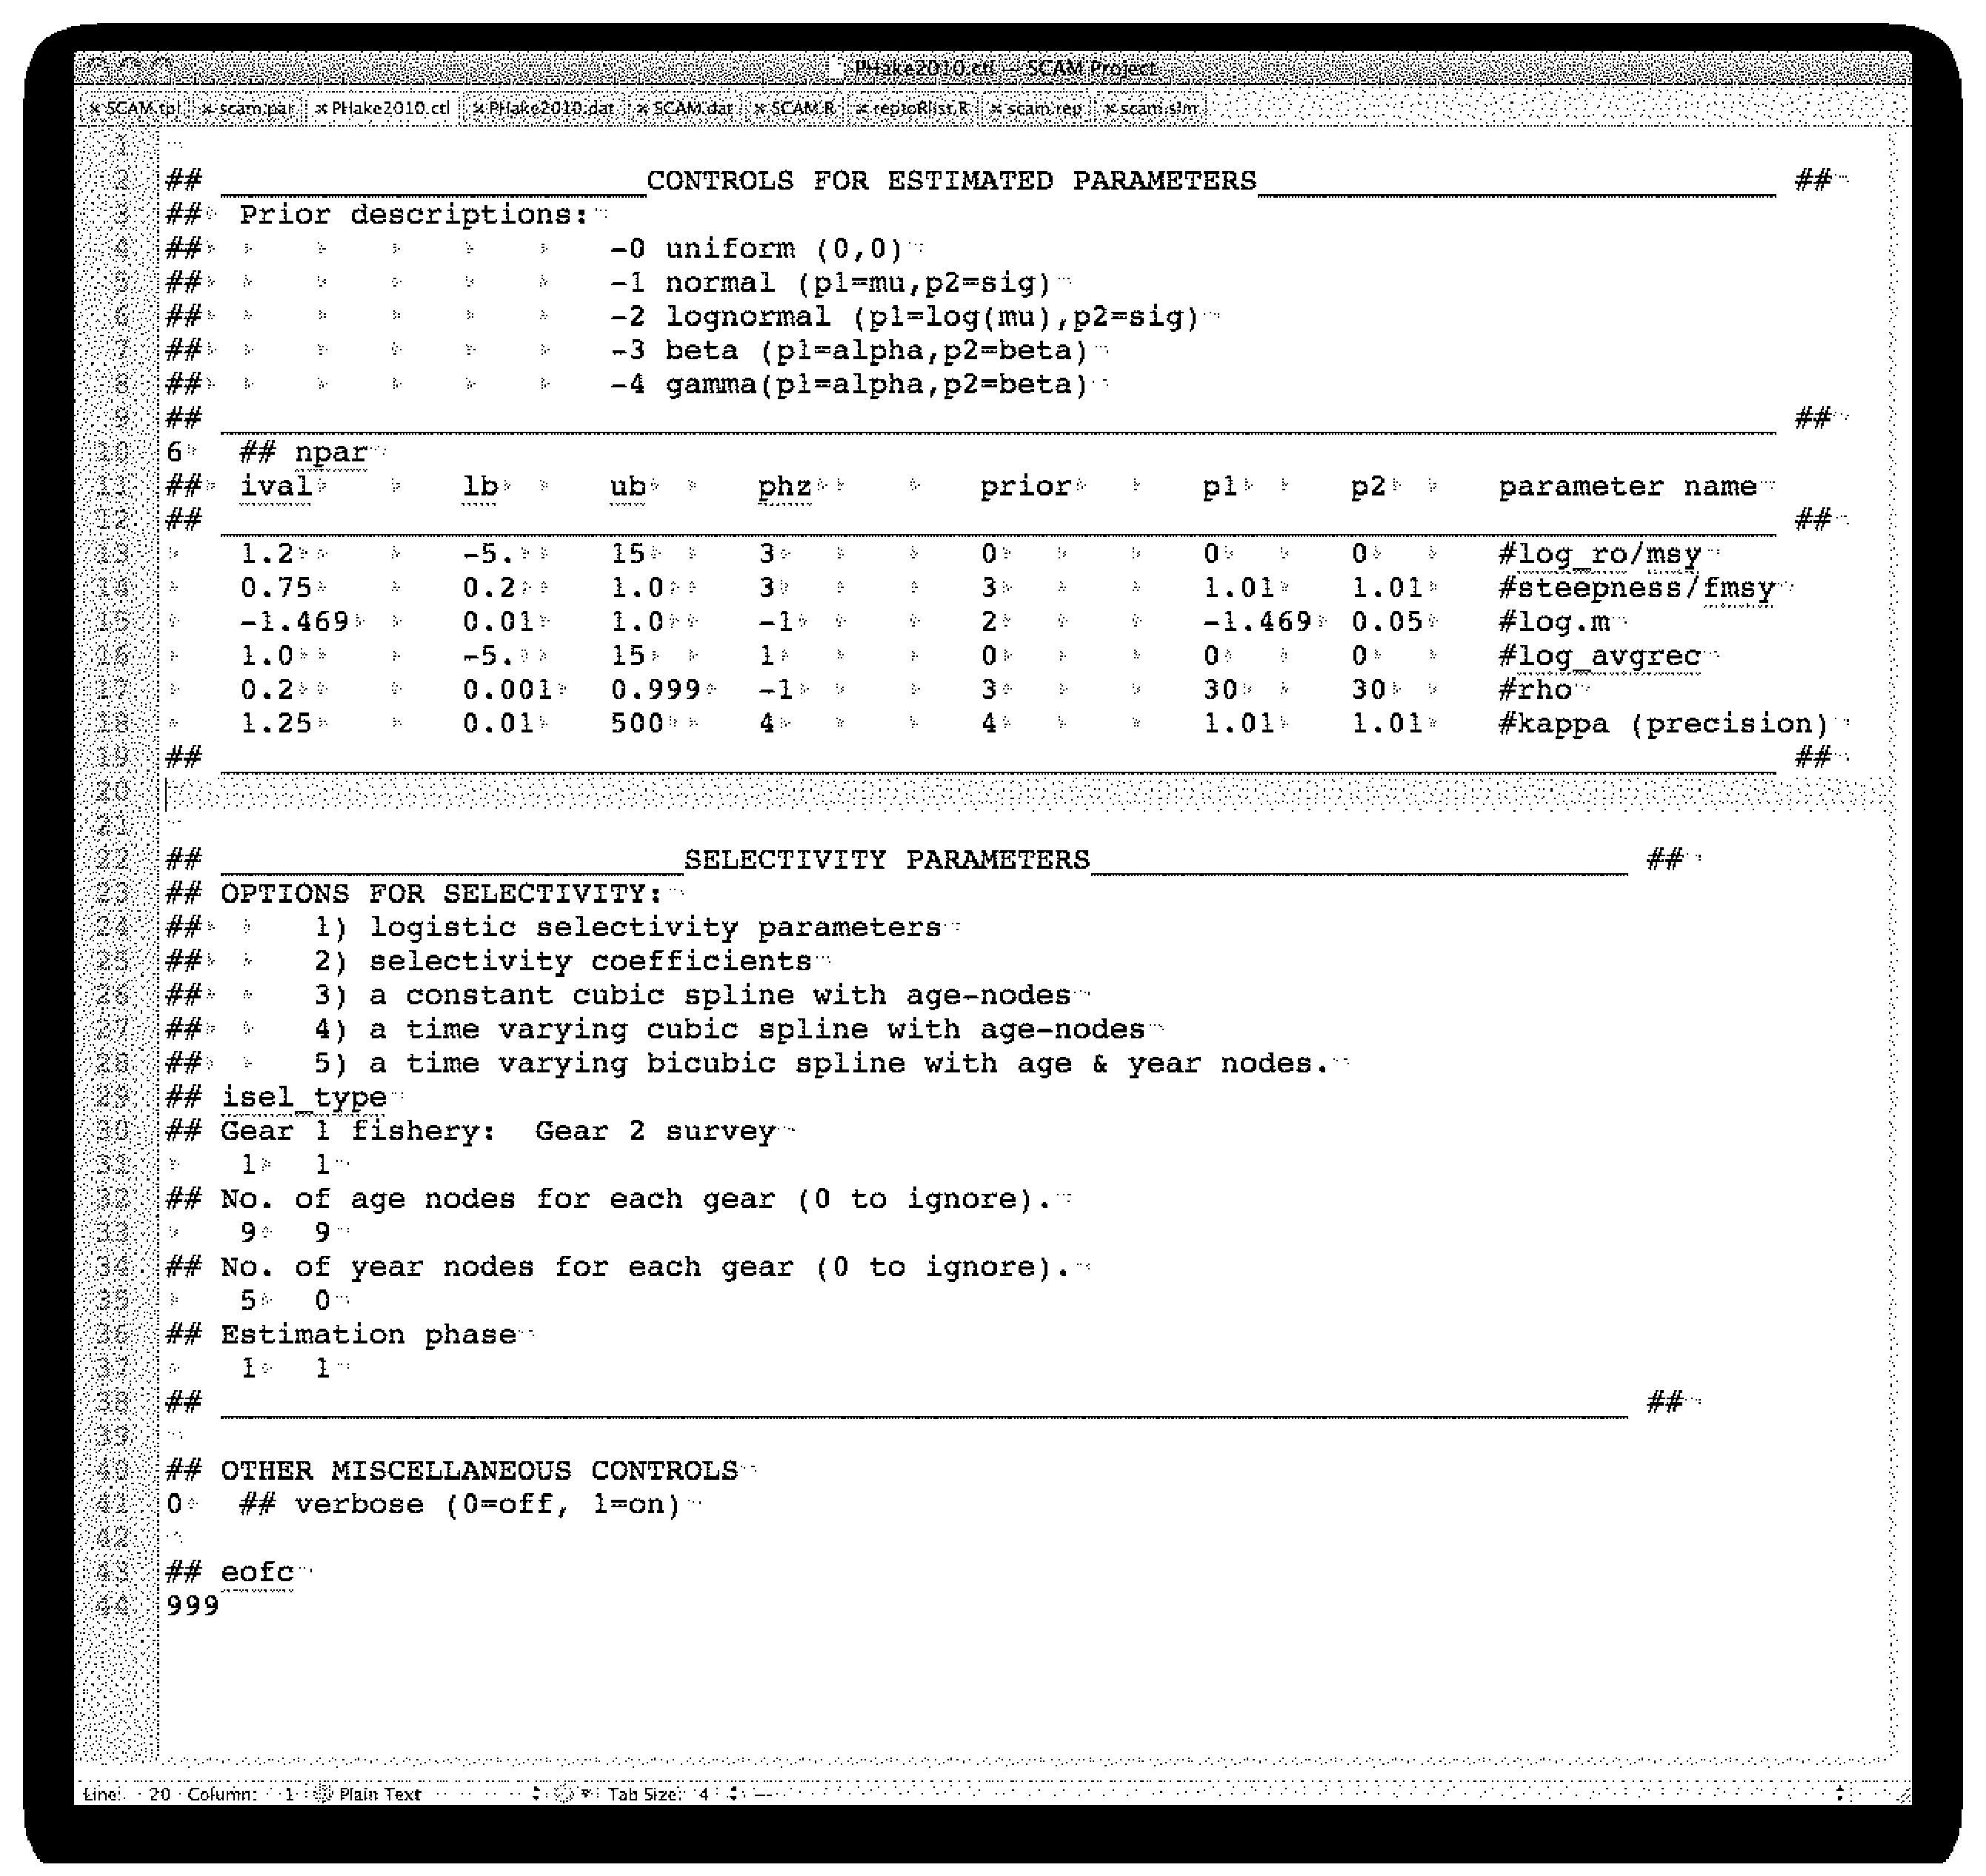
\includegraphics[width=\textwidth]{sc1.eps}\\
%	\caption{A screen shot of the example control file.}\label{Fig.control.file}
%\end{figure*}



\begin{multicols}{2}

\subsection{Command line options}
Currently there are two custom command line options available in \iscam\ in addition to the standard command line options provided by the AD Model Builder libraries (see help command line options -? for more information on the ADMB command line options). 

The custom command line options are:
\begin{description}
\item[-sim N] use this option turn the model into a simulation model, where N is the random number seed.

\item[-retro N] use the option for retrospective analysis where the last N years of data are ignored in the likelihood calculations.
\end{description}

There two random number seeds for the simulation model that the user should be aware of.  The first is if the random number seed is set to 000, then \iscam\ will actually simulate data with no errors whatsoever.  That is, the values of $\sigma$ and $\tau$ (observation error and process errors, respectively) will be set equal to 0 and the simulation model will run as a deterministic model with no observation errors in the relative abundance index or age composition data.  This option allows the user to check to ensure that the model parameters are in fact estimable with perfect information.


The second unique random seed number is 99, and this seed number is used for the simulation example in this manuscript.  It specifies a unique time-varying selectivity curve for the commercial fishery that goes from dome-shaped to asymptotic.

\subsubsection{Running the simulation model}

Again, one of the first steps in conducting any assessment should be to first run the model on simulated data with no error to be certain that the model is capable of estimating the specified model parameters.  To do so in \iscam\, the user simply needs to specify the command line option of \texttt{-sim 000}, where the `000' argument specifically instructs \iscam\ not to add any random variation to the observation or process errors.  Invoking this command line option will run \iscam\ as normal, where the data from the data file is first read into memory, then the information from the control file is then read in.  However, before proceeding straight into the non-linear parameter estimation procedure, \iscam\ first runs a simulation model based on the specified parameters listed in the control file.  This simulation model will then replace the existing data in memory with simulated data, then perform the non-linear parameter estimation procedure and attempt to estimate the model parameters.  If all is working well the estimated parameters listed in the parameter file should be very close, if not exactly, to the initial values specified in the control file.




\end{multicols}

%    %!TEX root = /Users/stevenmartell1/Documents/iSCAM-project/docs/iSCAM-guide/userGuide/usrGuide.tex
\section{Model Documentation} % (fold)
\label{sec:model_documentation}

\begin{multicols}{2}

The section contains the documentation in mathematical form of the underlying age-structured model, and its steady state version that is used to calculate reference points, the observation models used in predicting observations, and the components of the objective function that formulate the statistical criterion (i.e., the objective function) that is used to estimate model parameters.  All of the model equations are laid out in tables and are intended to represent the order of operations, or pseudocode, in which to implement the model.  \iscam\ was implemented in AD Model Builder version 10.0 \citep{otterResearch,ADMB2009}.

\subsection{List of symbols} % (fold)
\label{sub:list_of_symbols}
A documented list of symbols for the \iscam program is found in Table~\ref{tab:list_of_symbols} on page~\pageref{tab:list_of_symbols}.

% subsection list_of_symbols (end)


\end{multicols}


% List of symbols
\begin{center}
\begin{longtable}{lll}
\caption[list of symbols]{A list of symbols, constants and description for variables used in \iscam.} 
\label{tab:list_of_symbols} \tabularnewline

\hline 
\multicolumn{1}{l}{\textbf{Symbol}} & 
\multicolumn{1}{l}{\textbf{Value}} & 
\multicolumn{1}{l}{\textbf{Description}} \tabularnewline
\hline 
\endfirsthead

\multicolumn{3}{l}%
{{\bfseries \tablename\ \thetable{} -- continued from previous page}} 
\tabularnewline
\hline 
\multicolumn{1}{l}{\textbf{Symbol}} & 
\multicolumn{1}{l}{\textbf{Value}} & 
\multicolumn{1}{l}{\textbf{Description}} \tabularnewline
\hline 
\endhead

\hline \multicolumn{3}{l}{{Continued on next page}} \tabularnewline
\hline
\endfoot

\hline \hline
\endlastfoot

\multicolumn{3}{l}{\underline{Indexes}}\\
a & & index for age\\
t & & index for year\\
k & & index for gear\\
\multicolumn{3}{l}{\underline{Model dimensions}}\\
$\acute{a}, A$  & 2, 10         & youngest and oldest age class ($A$ is a plus group)\\
$\acute{t}, T$  & 1951, 2010    & first and last year of catch data\\
$K$             & 5             & Number of gears including survey gears\\
\multicolumn{3}{l}{\underline{Observations (data)}}\\
$C_{k,t}$       & & catch in weight by gear $k$ in year $t$\\
$I_{k,t}$       & & relative abundance index for gear $k$ in year $t$\\
$p_{k,t,a}$     & & observed proportion-at-age $a$ in year $t$ for gear $k$\\
\multicolumn{3}{l}{\underline{Estimated parameters}}\\
$R_o$               & & Age-$\acute{a}$ recruits in unfished conditions\\
$\kappa$            & & recruitment compensation\\
$M$                 & & instantaneous natural mortality rate \\
$\bar{R}$           & & average age-$\acute{a}$ recruitment from year $\acute{t}$ to $T$\\
$\ddot{R}$          & & average age-$\acute{a}$ recruitment in year $\acute{t}-1$\\
$\rho$              & & fraction of the total variance associated with observation error\\
$\vartheta$         & & total precision (inverse of variance) of the total error\\
$\vec{\gamma}_k$    & & vector of selectivity parameters for gear $k$\\
$\digamma_{k,t}$    & & logarithm of the instantaneous fishing mortality for gear $k$ in year $t$\\
$\ddot{\omega}_a$   & & age-$\acute{a}$ deviates from $\ddot{R}$ for year $\acute{t}$\\
$\omega_t$          & & age-$\acute{a}$ deviates from $\bar{R}$ for years $\acute{t}$ to $T$\\
$\varphi_t$         & & logarithm of annual change in natural mortality rate\\
\multicolumn{3}{l}{\underline{Standard deviations}}\\
$\sigma_M$          &0.1    & standard deviation in random walk for natural mortality\\
$\sigma$            &       & standard deviation for observation errors in survey index\\
$\tau$              &       & standard deviation in process errors (recruitment deviations)\\
$\sigma_C$          &0.0707 & standard deviation in observed catch by gear\\
\multicolumn{3}{l}{\underline{Residuals}}\\
$\delta_t$      &   & annual recruitment residual\\
$\eta_t$        &   & residual error in predicted catch\\


\end{longtable}
\end{center}


\subsection{Analytic methods: equilibrium considerations} % (fold)
\label{sub:analytic_methods_equilibrium_considerations}

\begin{multicols}{2}
\subsubsection{A steady-state age-structured model} % (fold)
\label{ssub:a_steady_state_age_structured_model}

% subsubsection a_steady_state_age_structured_model (end)

For the steady-state conditions represented in Table~\ref{tab:equilibrium_model}, we assume the parameter vector $\Theta$ in \eqref{T2.1} is unknown and would eventually be estimated by fitting \iscam\ to data.  For a given set of growth parameters and maturity-at-age parameters defined by \eqref{T2.3}, growth is assumed to follow von Bertalanffy \eqref{T2.4}, mean weight-at-age is given by the allometric relationship in \eqref{T2.5}, and the age-specific vulnerability is given by a logistic function \eqref{T2.6}.  Note, however, there are alternative selectivity functions implemented in \iscam, the logistic function used here is simply for demonstration purposes.  Mean fecundity-at-age is assumed to be proportional to the mean weight-at-age of mature fish, where maturity at age is specified by the parameters $\dot{a}$ and $\dot{\gamma}$ for the logistic function.

Survivorship for unfished and fished populations is defined by \eqref{T2.8} and \eqref{T2.9}, respectively.  It is assumed that all individuals ages $A$ and older (i.e., the plus group) have the same total mortality rate.  The incidence functions refer to the life-time or per-recruit quantities such as spawning biomass per recruit ($\phi_E$) or vulnerable biomass per recruit ($\phi_b$).  Note that upper and lower case subscripts denote unfished and fished conditions, respectively.  Spawning biomass per recruit is given by \eqref{T2.10}, the vulnerable biomass per recruit is given by \eqref{T2.11} and the per recruit yield to the fishery is given by \eqref{T2.11b}.  Unfished recruitment is given by \eqref{T2.12} and the steady-state equilibrium recruitment  for a given fishing mortality rate $F_e$ is given by \eqref{T2.13}.  Note that in \eqref{T2.13} we assume that recruitment follows either a  Beverton-Holt or a Ricker model in the forms:
\[
R_e=\begin{cases}
    \dfrac{s_o R_e \phi_e}{1+\beta R_e \phi_e},& \mbox{Beverton-Holt}\\[5ex]
    s_o R_e \phi_e \exp(-\beta R_e \phi_e)& \mbox{Ricker}
\end{cases}
\]
where the maximum juvenile survival rate is the same for both forms of the recruitment model and is given by:
\[
s_o = \kappa/\phi_E,
\]
and the density-dependent term is given by:
\[
\beta =\begin{cases}
    \dfrac{(\kappa-1)}{R_o\phi_E}, & \mbox{Beverton-Holt}\\[5ex]
    {\dfrac {\ln  \left( \kappa \right) }{R_{{o}}\phi_{{E}}}} & \mbox{Ricker}
\end{cases} 
\]
which simplifies to \eqref{T2.13}.
 The equilibrium yield for a given fishing mortality rate is \eqref{T2.14}.  These steady-state conditions are critical for determining various reference points such as \fmsy\ and \bmsy.  



%%%%%%%%%%%%%%%%%%%%%%%%%%%%%%%%%%%%%%%%%%%%%%%%%%%%%%%%%%%%%%%%%%%%%%
%%%%%%%%%%%%%%%%%%%%%%%%%%%%%%%%%%%%%%%%%%%%%%%%%%%%%%%%%%%%%%%%%%%%%%
\begin{tablehere}
  %\centering
\caption{Steady-state age-structured model assuming unequal
vulnerability-at-age, age-specific natural mortality, age-specific
fecundity and Beverton-Holt type recruitment.}\label{tab:equilibrium_model} 
\tableEq
    \begin{gather}
           \hline
        \mbox{Parameters} \nonumber \\
            \Theta = (B_o,\kappa,M_a,\hat{a},\hat{\gamma})      \label{T2.1}\\
            B_o>0; \kappa > 1; M_a > 0\\
            \Phi = (l_\infty, k, t_o,a,b,\dot{a},\dot{\gamma})  \label{T2.3}\\[1ex]
        %%
        %%
        \mbox{Age-schedule information} \nonumber\\
            l_a=l_\infty(1-\exp(-k(a-t_o)))                     \label{T2.4}\\
            w_a=a(l_a)^b                                        \label{T2.5}\\
            v_a=(1+\exp(-(\hat{a}-a)/\gamma))^{-1}              \label{T2.6}\\
            f_a=w_a(1+\exp(-(\dot{a}-a)/\dot{\gamma}))^{-1}     \label{T2.7}\\[1ex]
        %%
        %%
        \mbox{Survivorship} \nonumber\\
            \iota_a=\begin{cases} 1, &\quad a=1                 \label{T2.8}\\
            \iota_{a-1}e^{-M_{a-1}},&\quad a>1\\
            \iota_{a-1}/(1-e^{-M_a}),&\quad a=A \end{cases}\\
            \hat{\iota}_a=\begin{cases} 1, & a=1\\
            \hat{\iota}_{a-1}e^{-M_{a-1}-F_e v_{a-1}},& a>1\\
            \hat{\iota}_{a-1}e^{-M_{a-1}-F_e v_{a-1}}/(1-e^{-M_{a}-F_e v_{a}}),& a=A
            \end{cases}                                         \label{T2.9}\\[1ex]
        %%
        %%
        \mbox{Incidence functions} \nonumber \\
            \phi_E=\sum_{a=1}^\infty \iota_a f_a, \quad
            \phi_e=\sum_{a=1}^\infty \hat{\iota}_a f_a          \label{T2.10}\\
            \phi_B=\sum_{a=1}^\infty \iota_a w_a v_a, \quad
            \phi_b=\sum_{a=1}^\infty \hat{\iota}_a w_a v_a      \label{T2.11}\\
            \phi_q=\sum_{a=1}^\infty
                \frac{ \hat{\iota}_a w_a v_a}{M_a+F_ev_a}
                \left(1-e^{(-M_a-F_ev_a)}\right)                \label{T2.11b}\\[1ex]
        %%
        %%
        \mbox{Steady-state conditions} \nonumber \\
            R_o=B_o/ \phi_B                                     \label{T2.12}\\
            R_e=R_o\begin{cases}
            \dfrac{\kappa-\phi_E/\phi_e}{\kappa-1}&\mbox{Beverton-Holt}\\[2ex]
            \dfrac{\ln(\kappa)-\ln(\phi_E/\phi_e)}{\ln(\kappa)}& \mbox{Ricker}
            \end{cases}                                         \label{T2.13}\\
            C_e=F_e R_e \phi_q                                  \label{T2.14}\\[1ex]
        \hline \hline \nonumber
    \end{gather}
    \normalEq
\end{tablehere}
%%%%%%%%%%%%%%%%%%%%%%%%%%%%%%%%%%%%%%%%%%%%%%%%%%%%%%%%%%%%%%%%%%%%%%
%%%%%%%%%%%%%%%%%%%%%%%%%%%%%%%%%%%%%%%%%%%%%%%%%%%%%%%%%%%%%%%%%%%%%%
 

% subsection sub:analytic_methods_equilibrium_considerations (end)
%!TEX root = /Users/stevenmartell1/Documents/iSCAM-project/docs/iSCAM-guide/userGuide/usrGuide.tex
The concept of maximum sustainable yield, or MSY, is based on the notion that the underlying stock-size versus productivity can be estimated with some degree of certainty, and that this production function is stationary over time.  For a single fishing fleet, this can easily be represented as the equilibrium catch versus the equilibrium fishing effort (Fig. \ref{fig:iscamFigs_Fig1Quadplot}a), hereafter referred to as a yield curve. In the case of multiple fishing fleets, this yield curve  is not necessarily a smooth function as the total yield summed over all fleets is also a function of the fishing mortality exerted by each of the fleets.  In section \ref{ssub:msy_based_reference_points} a description of the equilibrium yields and MSY-based reference points is given, followed by a description of the numerical methods used to obtain MSY-based reference points when there are two or more fleets fishing simultaneously.

A special class library to implement the MSY-based reference point calculations was developed specifically for \iscam.  The C++ code for this class can be found in \texttt{msy.cpp}.


\subsubsection{MSY based reference points: single fleet} % (fold)
\label{ssub:msy_based_reference_points}



In the case of a single fishery \iscam\ calculates \fmsy\ based reference points by finding the value of $F_e$ that results in the zero derivative of \eqref{T2.14}.  This is accomplished numerically using a Newton-Raphson method where an initial guess for \fmsy\ is set equal to 1.0$M$, then use \eqref{eq1.1} to iteratively find \fmsy.  Note that the partial derivatives in \eqref{eq1.1} can be found in Table~\ref{tab:partial_derivatives}.

\begin{align}\label{eq1.1}
    F_{e+1}&=F_e - 
    \dfrac{ \dfrac{\partial C_e}{\partial F_e}}
    { \dfrac{\partial C_e^2}{\partial F_e^2}}\\
    \mbox{where}\nonumber\\
     \frac{\partial C_e}{\partial F_e} &=
    R_e \phi_q
    + F_e \phi_q \dfrac{\partial R_e}{\partial F_e}
    + F_e R_e \dfrac{\partial \phi_q}{\partial F_e} \nonumber\\
    \frac{\partial C_e^2}{\partial F_e^2} &=
    \phi_q \dfrac{\partial R_e}{\partial F_e}
   +  R_e \dfrac{\partial \phi_q}{\partial F_e}\nonumber
%    \frac{R_e \phi_q
%    + F_e \phi_q \dfrac{\partial R_e}{\partial F_e}
%    + F_e R_e \dfrac{\partial \phi_q}{\partial F_e}}
%    {\phi_q \dfrac{\partial R_e}{\partial F_e}
%    +  R_e \dfrac{\partial \phi_q}{\partial F_e}}.
\end{align}

The algorithm usually converges in less than 10 iterations depending on how close the initial guess of \fmsy\ is to the true value.  A maximum of 200 iterations are allowed in \iscam\ and if $\frac{\partial C_e}{\partial F_e}<1e-12$ it is assumed to be sufficiently close to zero and iterations will stop.  Note also, that this class object is only performed on data type variables and not differentiable variables within AD Model Builder.
 

\begin{figurehere}
    \centering
        \includegraphics[height=3in]{iscamFigs/Fig1Quadplot.pdf}
    \caption{Equilibrium yield (a), recruits (b), biomass (c) and
       spawner per recruit ($\phi_e/\phi_E$) (d) versus instantaneous
       fishing mortality $F_e$ for two different values of the recruitment
       compensation ratio ($\kappa=12$ solid lines, $\kappa=4$ dashed
       lines). Vertical lines in each panel correspond to \fmsy\ and
       horizontal lines correspond to various reference points that would
       achieve MSY.}
    \label{fig:iscamFigs_Fig1Quadplot}
\end{figurehere}

Given an estimate of \fmsy, other reference points such as MSY are calculated use the equations in Table-\ref{tab:equilibrium_model} where each of the expressions is evaluated at \fmsy.  A graphical representation of MSY based reference points for two alternative values of the recruitment compensation parameter $\kappa$ is show in Figure \ref{fig:iscamFigs_Fig1Quadplot}. All other parameters in the vectors $\Theta$ and $\Phi$ are identical between the two scenarios.  A lower recruitment compensation ratio (or a lower steepness value in the stock recruitment relationship) implies lower stock productivity or less resilience to fishing. Recruitment and biomass decrease at a much faster rate with increased fishing mortality in comparison to a stock with a higher recruitment compensation ratio. Note that the spawning potential ratio (SPR) curve is insensitive to the estimated value of recruitment compensation (steepness);  however, the SPR value at which MSY is achieved increases with lower recruitment compensation (Fig \ref{fig:iscamFigs_Fig1Quadplot}d).


%%%%%%%%%%%%%%%%%%%%%%%%%%%%%%%%%%%%%%%%%%%%%%%%%%%%%%%%%%%%%%%%%%%%%%
%%%%%%%%%%%%%%%%%%%%%%%%%%%%%%%%%%%%%%%%%%%%%%%%%%%%%%%%%%%%%%%%%%%%%%
\begin{tablehere}
  \centering
\caption{Partial derivatives, based on components in Table
\ref{tab:equilibrium_model}, required for the numerical calculation of \fmsy\ using \eqref{eq1.1}.}\label{tab:partial_derivatives} \tableEq
    \begin{gather}
        \hline
        \mbox{Mortality \& Survival} \nonumber \\
        Z_{a}=M_a+F_ev_a                                \label{T3.1} \\
        S_{a}=1-e^{-Z_a}                                \label{T3.2}\\[1ex]
        %%
        %%
        \mbox{Partial for survivorship} \nonumber \\
        \frac{\partial \hat{\iota}_a}{\partial F_e} =
        \begin{cases}
          0,& a=1                                       \label{T3.3}\\
          e^{-Z_{a-1}}\left(\dfrac{\partial \hat{\iota}_{a-1}}{\partial F_e}
           -\hat{\iota}_{a-1}v_{a-1}\right),& 1<a<A\\
           \dfrac{\dfrac{\partial \hat{\iota}_{a-1}}{\partial F_e}}
           {1-e^{-Z_a}} -
           \dfrac{\hat{\iota}_{a-1} e^{-Z_{a-1}} v_a e^{-Z_a}}
           {(1-e^{-Z_a})^2}, &a=A
        \end{cases} \\[1ex]
%%        \frac{\partial \hat{\iota}_a}{\partial F_e} =
%%        \begin{cases}
%%          0,& a=1 \label{T3.3}\\
%%          e^{-Z_{a-1}}\left(\dfrac{\partial \hat{\iota}_{a-1}}{\partial F_e}
%%           -\hat{\iota}_{a-1}v_{a-1}\right),& a>1
%%        \end{cases} \\[1ex]
        %%
        %%
        \mbox{Partials for incidence functions} \nonumber \\
        \frac{\partial \phi_e}{\partial F_e}=
            \sum_{a=1}^\infty f_a \frac{\partial \hat{\iota}_a}{\partial
            F_e}                                        \label{T3.4}\\
        %%
        %%
        \frac{\partial \phi_q}{\partial F_e}=
            \sum_{a=1}^\infty \frac{w_av_a S_a}{Z_a}
             \frac{\partial \hat{\iota}_a}{\partial F_e}
             +\frac{\hat{\iota}_a w_av_a^2}{Z_a}\left(e^{-Z_a}-\frac{S_a}{Z_a} \right)
                                                            \label{T3.5}\\[1ex]
        %%
        %%
        \mbox{Partial for recruitment} \nonumber\\
        \frac{\partial R_e}{\partial F_e}=\frac{R_o}{\kappa-1}
        \frac{\phi_E}{\phi_e^2} \frac{\partial \phi_e}{\partial
        F_e}                                                \label{T3.6}\\[1ex]
        \hline \hline \nonumber
    \end{gather}

    \normalEq
\end{tablehere}
%%%%%%%%%%%%%%%%%%%%%%%%%%%%%%%%%%%%%%%%%%%%%%%%%%%%%%%%%%%%%%%%%%%%%%
%%%%%%%%%%%%%%%%%%%%%%%%%%%%%%%%%%%%%%%%%%%%%%%%%%%%%%%%%%%%%%%%%%%%%%

% subsubsection msy_based_reference_points (end)

\subsubsection{MSY Based Reference Points: two or more fleets} % (fold)
\label{ssub:msy_based_reference_points_two_or_more_fleets}

In the case where there are two or more fishing fleets with distinctly different selectivity curves for each of the fleets, determination \fmsy for each of the fleets is a bit more complicated.  The first major complication is solving the catch equation where \eqref{T2.14} now involves a summation term over different fishing fleets.  The second complication is how should the total catch (summed over fleets) be allocated to each of the fleets.  In the special case where selectivity for each of the fishing fleets is identical, an equal proportion of the total catch allocated to each of those fleets also corresponds to the same fishing mortality for each of those fleets.  In the more common case where selectivity differs among fleets, the fishing mortality rates associated with equal allocations would also differ.  Consider the following example, if you have a purse seine fleet that harvests small young tuna, and a long-line fleet that harvest the same stock but selects larger older tuna. If each of these two fleets are allocated a 50:50 share, the instantaneous fishing mortality rate would have to be much higher for the long-line gear relative to the purse seine gear that harvest the more abundance small/young tuna.  Regarding the first complication, the following description is based on the assumption is that the total catch summed over all fleets is maximized, and that allocation of total catch is a secondary issue. For the second complication, a vector of fishing mortality rate multipliers is used to adjust fleet specific fishing mortality rates to satisfy catch allocations.  Lastly, a third complication pertains to the accounting of mature numbers-at-age at the time of spawning and how much of the total annual mortality occurs prior to spawning. 


% From msy.cpp
The steady-state catch equation for fleet $k$, with an instantaneous fishing mortality rate $F_k$, is given by:
\begin{align}
	C_{k} &= F_k R_e \phi_{q,k} \label{eq:C_k}\\
	\mbox{where}\nonumber\\
	R_e &= \frac{R_o (\kappa-\phi_E/\phi_e)}{\kappa-1} \label{eq:R_e}\\  %ro*(kappa-m_phie/phif) / km1;
	\phi_{q,k} &= \sum_j = \frac{e^{-M(j-1)}V_{k,j}w_a (1-e^{-M-\sum_k F_k V_{k,j} })}{M+\sum_k F_k V_{k,j}} \label{eq:phi_qk}
\end{align}

Although the catch equation appears relatively simple, there are two key points to note about the equilibrium recruitment $R_e$ and the yield per recruit $\phi_{q,k}$ in \eqref{eq:R_e} and \eqref{eq:phi_qk}, respectively. First, \eqref{eq:R_e} is a function of the eggs per recruit under fished conditions $\phi_e$, which is based on the survivorship which depends on the fishing mortality rates of all gears.  Second, the yield per recruit in \eqref{eq:phi_qk} is a function of the total mortality rate which involves the summation over gears.

The maximum total yield summed over all $k$ fleets occurs under the following condition:
\begin{equation}
	0 = \sum_k \frac{\partial C_k}{\partial F_k}  \label{eq:Catch_derivative}
\end{equation}
and thus the goal is to find a vector of steady-state fishing mortality rates $F_k$ to satisfy \eqref{eq:Catch_derivative}.  


% subsubsection msy_based_reference_points_two_or_more_fleets (end)


\subsubsection{Reference points for multiple fisheries with fixed allocation} % (fold)
\label{ssub:reference_points_for_multiple_fisheries}
% It is common that a single stock of fish is prosecuted by many different types of fishing gears that have differing selectivities.  In such cases, the definition of MSY is based on the sum of catches from each of the participating fleets and how much of the total catch is taken, or allocated, to specific sectors.  For such cases, it is still possible to calculate MSY-based reference points provided that allocation to each of the gear types is specified \emph{a priori}.

To determine MSY-based reference points for 2 or more gear types (e.g.,  purse seine and gillnet fisheries for Pacific herring in British Columbia), \iscam\ requires an allocation for each of the defined fleets.  Allocation is specified in the data file (see sub section \ref{sub:the_data_file}).  This allocation is initially used set a series of F-multipliers ($\lambda_k$) for each gear and \eqref{T2.14} becomes a vector of catches:
\begin{align}
	C_{e,k} &= F_e \lambda_k R_e \phi_{q,k} \label{eq:12} \\
	&\mbox{where the per-recruit yield for gear $k$ is:} \nonumber \\
	Z_a &= M+F_e\sum_k \lambda_kv_{k,a}\label{eq:13}\\
	\phi_{q,k}&=\sum_{a=1}^\infty
        \frac{ \hat{\iota}_a \lambda_k w_a v_{k,a}}{Z_a}
        \left(1-e^{Z_a}\right)\label{eq:14}\\
    &\mbox{with the added constraint} \nonumber\\
    \sum_k \lambda_k &= N \label{eq:15}\quad \mbox{where $N$ is the number of gears.}
\end{align}

The constraint in \eqref{eq:15} defines $F_e\lambda_k$ as the fishing mortality rate for gear $k$ where $\lambda_k$ is a multiple of the average fishing mortality rate of all gears.  To ensure that each gear achieves the specified allocation for a given average fishing mortality rate $F_e$, the multipliers are determined iteratively where $\lambda_k$ is updated using:
\begin{align}
	\lambda_k^{(i+1)} &= \lambda_k^{(i)} \frac{a_k}{p_k} \label{eq:16}\\
	&\mbox{where $a_k$ is the allocation for gear $k$, and:}\nonumber\\
	p_k &= \frac{C_{e,k}}{\sum_k C_{e,k}}\label{eq:17}
\end{align}
Depending on the differences in selectivities and allocations between the gear types, this algorithm converges roughly 7-15 iterations.  From here the same Newton-Raphson algorithm is used to determine the average fishing mortality rate $F_e$ that would maximize the sum of catches over the multiple gears.  
% subsubsection reference_points_for_multiple_fisheries (end)



\subsection{MSY-based reference points for multiple fisheries} % (fold)
\label{sub:msy_based_reference_points_for_multiple_fisheries}

In cases where there are two or more fishing fleets that harvest the same stock (intentionally or taken as bycatch), the differences in selectivity among these gears will ultimately affect the fishing mortality rates associated with long-term sustainable yields or MSY for each of the participating fleets.  For example, global tuna fisheries are taken primarily by two gear types, pelagic longlines which harvest larger/older tuna, and purse seine's which harvest younger tuna usually aggregated around Fish Aggregating Devices (FADs).  The longline fishery has been in operation since the 1950s (even longer, but the available data date back to the 1950s), and the industrial purse seine fishery developed in the 1980s.  If in fact the longline fishery was fully utilized by the 1980s, then the impacts of increased mortality on younger tuna from the purse seine fleet would reduce the available surplus for the longline fishery.

To estimate what the appropriate MSY-based fishing mortality rates for two or more fishing gears that harvest the same stock of fish, the catch equations for each fleet must be simultaneously solved in order to find the appropriate vector of fishing mortality rates that that maximizes the yields for each fleet.  The steady-state, or equilibrium, catch equation for a given fishing gear $k$ is given by:
\begin{equation}\label{eq:equilYield}
	 Y_{k} = \sum_j\frac{N_j F_k v_{k,j} w_j (1-\exp(-M-\sum_k F_k v_{k,j}))} {M + \sum_k F_k v_{k,j}},
\end{equation}
where $F_k$ is the fishing mortality rate imposed by gear $k$, M is the instantaneous natural mortality rate, $v_{k,j}$ is the age-specific selectivity for gear $k$ and age $j$, and $w_j$ and $N_j$ are the average weight-at-age and numbers-at-age, respectively.  Note that if $k>1$, then \eqref{eq:equilYield} represents of system of nonlinear equations where the roots of these equations $\left(\frac{\partial Y_k}{\partial F_k}=0\right)$ are found with Newton-Raphson.

\subsubsection{Algorithm for estimating \fmsy\ for multiple fleets} % (fold)
\label{ssub:algorithm_for_estimating_fmsy_for_multiple_fleets}


% subsubsection algorithm_for_estimating_fmsy_for_multiple_fleets (end)

% subsection msy_based_reference_points_for_multiple_fisheries (end)





\end{multicols}




\subsection{Analytic methods: state-dynamics} % (fold)
\label{sub:analytic_methods_state_dynamics}


\begin{multicols}{2}
The estimated parameter vector in \iscam\ is defined in \eqref{T4.1}, where $R_0, \kappa$ and $M$ are the leading unknown population parameters that define the overall population scale in the form of unfished recruitment and productivity in the form of recruitment compensation and natural mortality.  The total variance $\vartheta^2$ and the proportion of the total variance that is associated with observation errors $\rho$ are also estimated, then the variance is partitioned into observation errors ($\sigma^2$) and process errors ($\tau^2$) using \eqref{T4.2}.

The unobserved state variables \eqref{T4.3} include the numbers-at-age year year $t$ ($N_{t,a}$), the spawning stock biomass ($B_t$) and the total age-specific total mortality rate ($Z_{t,a}$).

The initial numbers-at-age in the first year \eqref{T4.4} and the annual recruits \eqref{T4.5} are treated as estimated parameters and used to initialize the numbers-at-age matrix.  Age-specific selectivity for gear type $k$ is a function of the selectivity parameters $\gamma_k$ \eqref{T4.6}, and the annual fishing mortality for each gear $k$ in year $t$ ($\digamma_{k,t}$).  The vector of log fishing mortality rate parameters $\digamma_{k,t}$ is a bounded vector with a minimum value of -30 and an upper bound of 3.0.  In arithmetic space this corresponds to a minimum value of 9.36e-14 and a maximum value of 20.01 for annual fishing mortality rates.  In years where there are 0 reported catches for a given fleet, no corresponding fishing mortality rate parameter is estimated and the implicit assumption is there was no fishery in that year.

There is an option to treat natural mortality as a random walk process \eqref{T4.6b}, where the natural mortality rate in the first year is the estimated leading parameter \eqref{T4.1} and in subsequent years the mortality rate deviates from the previous year based on the estimated deviation parameter $\varphi_t$.  If the mortality deviation parameters are not estimated, then $M$ is assumed to be time invariant.

State variables in each year are updated using equations \ref{T4.8}--\ref{T4.11}, where the spawning biomass is the product of the numbers-at-age and the mature biomass-at-age \eqref{T4.8}.  The total mortality rate is given by \eqref{T4.9}, and the total catch (in weight) for each gear is given by \eqref{T4.10} assuming that both natural and fishing mortality occur simultaneously throughout the year.  The numbers-at-age are propagated over time using \eqref{T4.11}, where members of the plus group (age $A$) are all assumed to have the same total mortality rate.  

Recruitment to age $k$ can follow either a Beverton-Holt model \eqref{T4.12} or a Ricker model \eqref{T4.13} where the maximum juvenile survival rate ($s_o$) in either case is defined by $s_o=\kappa/\phi_E$.  For the Beverton-Holt model, $\beta$ is derived by solving \eqref{T4.12} for $\beta$ conditional on estimates of $\kappa$ and $R_o$:
\[
\beta = \frac{\kappa-1}{R_o \phi_E},
\]
and for the Ricker model this is given by:
\[
\beta = \frac{\ln(\kappa)}{R_o \phi_E}
\]

%%%%%%%%%%%%%%%%%%%%%%%%%%%%%%%%%%%%%%%%%%%%%%%%%%%%%%%%%%%%%%%%%%%%%%%%
%%%%%%%%%%%%%%%%%%%%%%%%%%%%%%%%%%%%%%%%%%%%%%%%%%%%%%%%%%%%%%%%%%%%%%%%
\begin{tablehere}
  \centering
\caption{Statistical catch-age model using the Baranov catch.}
\label{tab:statistical_catch_age_model}
\tableEq
    \begin{align}
        \hline \nonumber \\
        &\mbox{Estimated parameters} \nonumber\\
        \begin{split}
        \Theta&= 
                (R_0,\kappa,M,\bar{R},\rho,\vartheta^2,\gamma_{k},%\bar{F}_k,
                \digamma_{k,t},\\
        &\quad \{\omega_t\}_{t=1-A}^{t=T},
                \{\varphi_t \}_{t=2}^T)
    \end{split} \label{T4.1}\\
        \sigma^2&=\rho /\vartheta^2, \quad
        \tau^2=(1-\rho)/\vartheta^2\label{T4.2}\\[1ex]
        %\vartheta^2=\sigma^2+\tau^2, \quad
        %\rho=\frac{\sigma^2}{\sigma^2+\tau^2}\label{T4.3}\\[1ex]
        %%
        %%
        &\mbox{Unobserved states} \nonumber\\
        &N_{t,a},B_t,Z_{t,a}    \label{T4.3}\\
    %%
    %%          
        &\mbox{Initial states} \nonumber\\
        %v_a=\left[1+e^{-(\hat{a}-a)/\hat{\gamma}}\right]^{-1}\label{T4.7}\\
        N_{t,a}&=\bar{R}e^{\omega_{t-a}} \exp(-M_t)^{(a-1)};\quad t=1;  2\leq a\leq A \label{T4.4}\\
        N_{t,a}&=\bar{R}e^{\omega_{t}} ;\quad 1\leq t\leq T;  a=1 \label{T4.5}\\
        v_{k,a}&=f(\gamma_k) \label{T4.6}\\
        M_t &= M_{t-1} \exp(\varphi_t), \quad t>1 \label{T4.6b}\\
        F_{k,t}&=\exp(\digamma_{k,t}) \label{T4.7}\\[1ex]
        %%
        %%
        &\mbox{State dynamics (t$>$1)} \nonumber\\
        B_t&=\sum_a N_{t,a}f_a \label{T4.8}\\
        Z_{t,a}&=M_t+\sum_k F_{k,t} v_{k,t,a}\label{T4.9}\\
        \hat{C}_{k,t}&=\sum _ a\frac {N_{{t,a}}w_{{a}}F_{k,t} v_{{k,t,a}}
        \left( 1-{e^{-Z_{t,a}}} \right) }{Z_{t,a}}^{\eta_t} \label{T4.10}\\
        %F_{t_{i+1}}= \ F_{t_{i}} -\frac{\hat{C}_t-C_t}{\hat{C}_t'} \label{T4.12}\\
        N_{t,a}&=\begin{cases}
            %\dfrac{s_oE_{t-1}}{1+\beta E_{t-1}} \exp(\omega_t-0.5\tau^2) &a=1\\ \\
            N_{t-1,a-1} \exp(-Z_{t-1,a-1}) &a>1\\
            N_{t-1,a} \exp(-Z_{t-1,a}) & a=A
        \end{cases}\label{T4.11}\\[1ex]
        %%
        %%
        &\mbox{Recruitment models} \nonumber\\
        R_t &= \frac{s_oB_{t-k}}{1+\beta B_{t-k}}e^{\delta_{t}-0.5\tau^2} \quad \mbox{Beverton-Holt} \label{T4.12}\\
        R_t &= s_oB_{t-k}e^{-\beta B_{t-k}+\delta_t-0.5\tau^2} \quad \mbox{Ricker} \label{T4.13}\\
    %%        \mbox{Residuals \& predicted observations} \nonumber\\
    %%        \epsilon_t=\ln\left(\frac{I_t}{B_t}\right)-\frac{1}{n}\sum_{t \in I_t}\ln\left(\frac{I_t}{B_t}\right)\label{T4.15}\\
    %%        \hat{A}_{t,a}=\dfrac{N_{t,a}\dfrac{F_tv_a}{Z_{t,a}}\left(1-e^{-Z_{t,a}}\right)}
    %%        {\sum_a N_{t,a}\dfrac{F_tv_a}{Z_{t,a}}\left(1-e^{-Z_{t,a}}\right)}\label{T4.16}\\
        \hline \hline \nonumber
    \end{align}

    \normalEq
\end{tablehere}
%%%%%%%%%%%%%%%%%%%%%%%%%%%%%%%%%%%%%%%%%%%%%%%%%%%%%%%%%%%%%%%%%%%%%%%%
%%%%%%%%%%%%%%%%%%%%%%%%%%%%%%%%%%%%%%%%%%%%%%%%%%%%%%%%%%%%%%%%%%%%%%%%





\subsubsection{Options for selectivity ($v_{k,t,a}$)} \label{ModelDocSelectivity}

At present, there are six alternative age-specific selectivity options in \iscam.  The simplest of the selectivity options is a simple logistic function with two parameters where it is assumed that selectivity is time-invariant.  The more complex selectivity options assume that selectivity may vary over time a may have as many as (A-1)$\cdot$T parameters.  For time-varying selectivity, cubic and bicubic splines are used to reduce the number of estimated parameters.  Prior to parameter estimation, \iscam\ will determine the exact number of selectivity parameters that need to be estimated based on which selectivity option was chosen for each gear type.  It is not necessary for all gear types to have the same selectivity option.  For example it is possible to have a simple two parameter selectivity curve for say a survey gear, and a much more complicated selectivity option for a commercial fishery.

\paragraph{Logistic selectivity} 
The logistic selectivity option is a two parameter model of the form
\[
v_a = \frac{1}{1+ \exp{(-(a-\mu_{a})/\sigma_a)}}
\]
where $\mu_a$ and $\sigma_a$ are the two estimated parameters representing the age-at-50\% vulnerability and the standard deviation, respectively.

\paragraph{Age-specific selectivity coefficients}
The second option also assumes that selectivity is time-invariant and estimates at total of $A$-1 selectivity coefficients, where the plus group age-class is assumed to have the same selectivity as the previous age-class.  For example, if the ages in the model range from 1 to 15 years, then a total of 14 selectivity parameters are estimated, and age-15+ animals will have the same selectivity as age-14 animals.

When estimating age-specific selectivity coefficients, there are two additional penalties that are added to the objective function that control how much curvature there is and limit how much dome-shaped can occur.  To penalize the curvature, the square of the second differences of the vulnerabilities-at-age are added to the objective function: 
\[
\lambda_k^{(1)} \sum_{a=2}^{A-1}(v_{k,a} - 2v_{k,a-1} + v_{k,a-2})^2
\]
The dome-shaped term penalty as:
\[
\begin{cases}
\lambda_k^{(2)} \sum_{a=1}^{A-1}(v_{k,a} - v_{k,a+1})^2& \mbox(if) v_{k,a+1}< v_{k,a}\\
0 & \mbox(if) v_{k,a+1}\geq v_{k,a}
\end{cases}
\]
For this selectivity option the user must specify the relative weights ($\lambda_k^{(1)},\lambda_k^{(2)}$) to add to these two penalties.

\paragraph{Cubic spline interpolation}
The third option also assumes time-invariant selectivity and estimates a selectivity coefficients for a series age-nodes (or spline points) and uses a natural cubic spline to interpolate between these nodes (Figure \ref{Fig2}). Given $n+1$ distinct knots $x_i$, selectivity can be interpolated in the intervals defined by
\[
S(x) = \begin{cases}
    S_0(x) & x \in [x_0,x_1]\\
    S_1(x) & x \in [x_1,x_2]\\
    ...\\
    S_{n-1}(x) & x \in [x_{n-1},x_n]
\end{cases}
\]
where  $S''(x_0) = S''(x_n)=0$  is the condition that defines a natural cubic spline.
\begin{figurehere}
    \centering
    % Requires \usepackage{graphicx}
    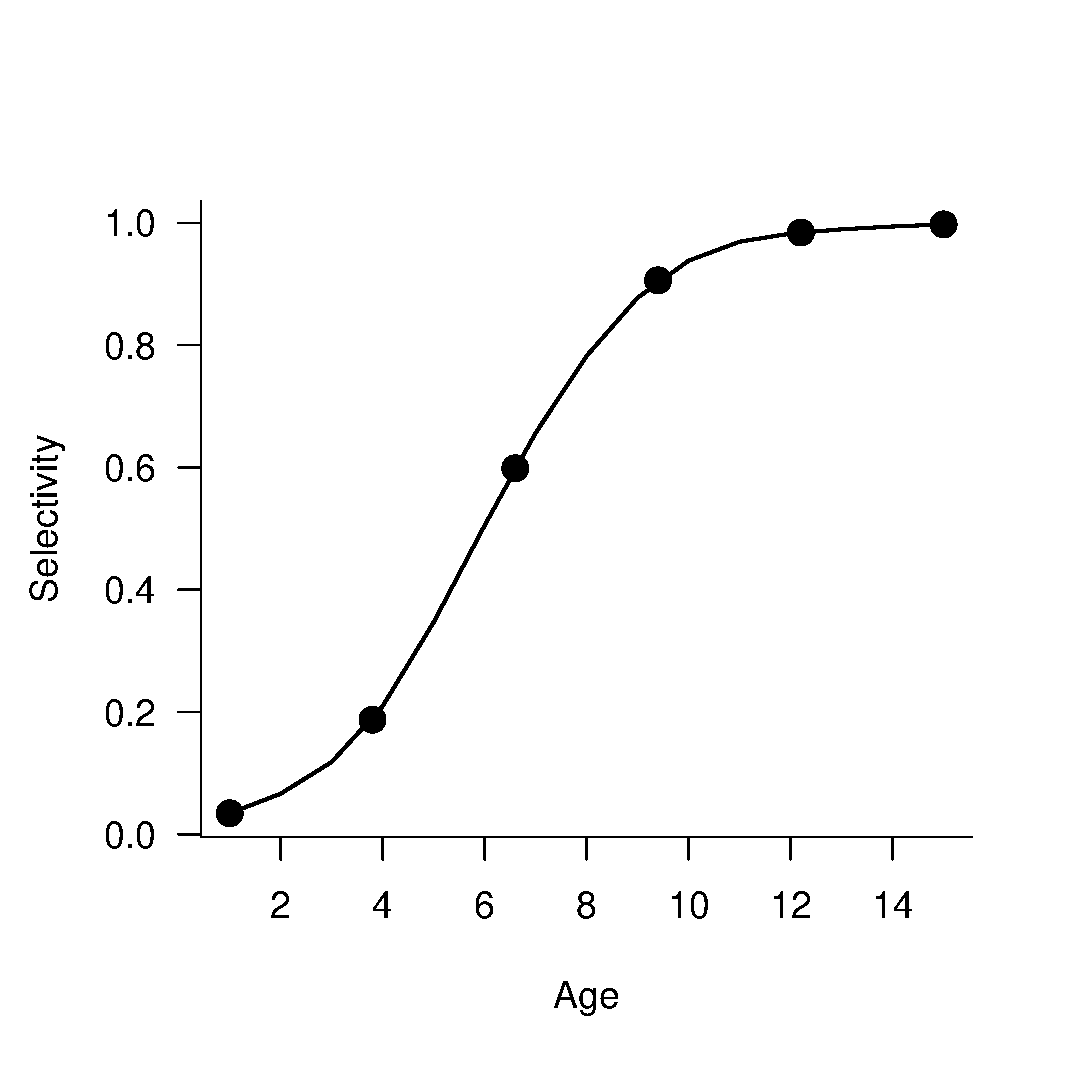
\includegraphics[width=\columnwidth]{iscamFigs/SplineEg.eps}\\
    \caption{Example of a natural cubic spline interpolation for estimating selectivity coefficients.  In \iscam\ the user specifies the number of nodes (circles) to estimate; then age-specific selectivity coefficients are interpolated using a natural cubic spline.}\label{Fig2}
\end{figurehere}

The same penalty functions for curvature and dome-shaped selectivity are also invoked for the cubic spline interpolation of selectivity.

\paragraph{Time-varying selectivity with cubic spline interpolation} A fourth option allows for cubic spline interpolation for age-specific selectivity  in each year.  This option adds a considerable number of estimated parameters but the most extreme flexibility.  For example, given 40 years of data and estimated 5 age nodes, this amounts 200 (40 years times 5 ages) estimated selectivity parameters.  Note that the only constraints at this time are the dome-shaped penalty and the curvature penalty; there is no constraint implemented for say a random walk (first difference) in age-specific selectivity).  As such this option should only be used in cases where age-composition data is available for every year of the assessment.

\paragraph{Bicubic spline to interpolate over time and ages}  The fifth option allows for a two-dimensional interpolation using a bicubic spline (Figure \ref{Fig3}).  In this case the user must specify the number of age and year nodes.  Again the same curvature and dome shaped constraints are implemented.  It is not necessary to have age-composition data each and every year as in the previous case, as the bicubic spline will interpolate between years.  However, it is not advisable to extrapolate selectivity back in time or forward in time where there are no age-composition data unless some additional constraint, such as a random-walk in age-specific selectivity coefficients is implemented (as of \today, this has not been implemented).

\begin{figure*}[!tbp]
    % Requires \usepackage{graphicx}
    \centering
    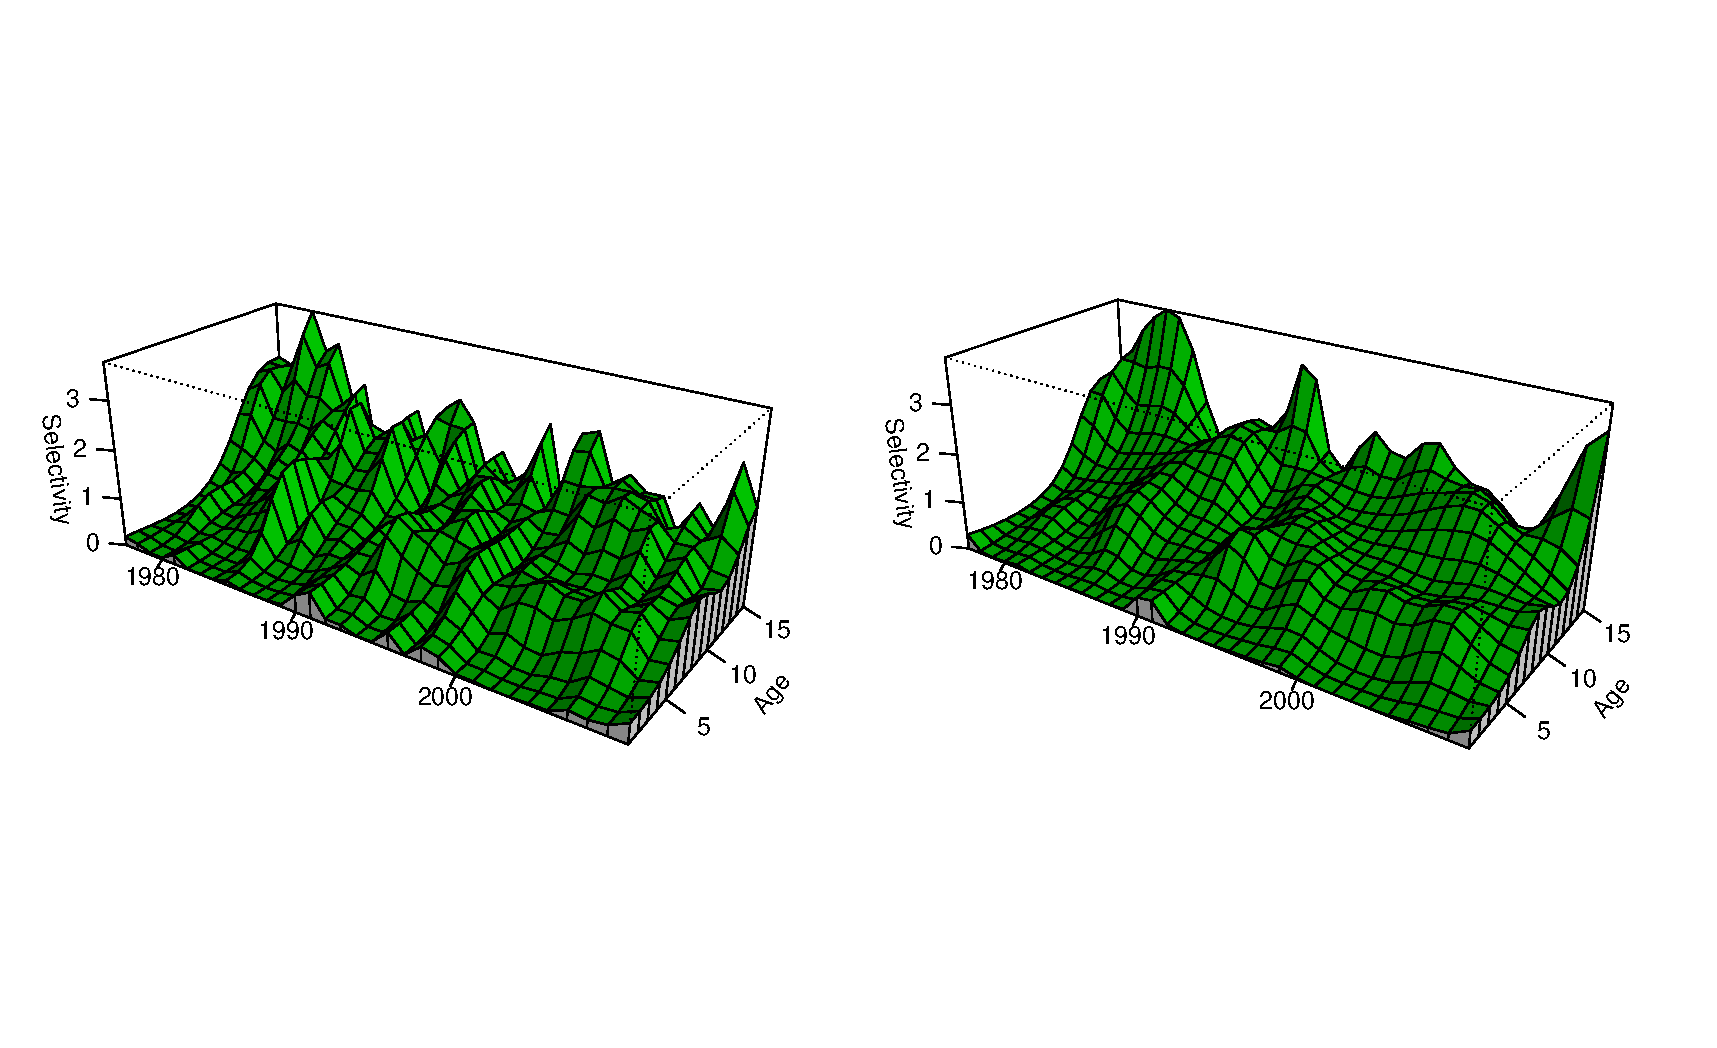
\includegraphics[width=0.9\textwidth]{iscamFigs/BicubicEg.eps}\\
    \caption{Example of a time-varying cubic spline (left) and bicubic spline (right) interpolation for selectivity as applied to the Pacific hake data. The panel on the left contains 165 estimated selectivity parameters and the bicubic interpolation estimates 85 selectivity parameters, or 5 age nodes and 17 year nodes. There are 495 actual nodes being interpolated.}\label{Fig3}
\end{figure*}
%\end{multicols}

\subsection{Residuals, likelihoods \& objective function value components}
%\begin{multicols}{2}
There are 3 major components to the overall objective function that are minimized while \iscam\ is performing maximum likelihood estimation.  These components consist of the likelihood of the data, prior distributions and penalty functions that are invoked to regularize the solution during intermediate phases of the non-linear parameter estimation.  This section discusses each of these in turn, starting first with the residuals between observed and predicted states followed by the negative loglikelihood that is minimized.

\subsubsection{Catch data}
It is assumed that the measurement errors in the catch observations are log-normally distributed, and the residuals is given by:
\begin{equation}\label{eq2}
\eta_{k,t}=\ln(C_{k,t}+o) -  \ln(\hat{C}_{k,t}+o),
\end{equation}
where $o$ is  a small constant (1.e-10) to ensure the residual is defined in the case of a 0 catch observation.  The residuals are assumed to be normally distributed with a user specified standard deviation $\sigma_{C}$.  At present, it is assumed that observed catches for each gear $k$ is assumed to have the same standard deviation.  To aid in parameter estimation, two separate standard deviations are specified in the control file: the first is the assumed standard deviation used in the first, second, to N-1 phases, and the second is the assumed standard deviation in the last phase.  The negative loglikelihood (ignoring the scaling constant) for the catch data is given by:
\begin{equation}\label{eq3}
\ell_C = \sum_k\left[  T_k\ln(\sigma_C)+\frac{\sum_t(\eta_{k,t})^2}{2\sigma_C^2}\right],
\end{equation}
where $T_k$ is the total number of catch observations for gear type $k$.


\subsubsection{Relative abundance data}
The relative abundance data are assumed to be proportional to biomass that is vulnerable to the sampling gear:
\begin{equation}\label{eq4}
 V_{k,t} = \sum_a N_{t,a} e^{-\lambda_{k,t} Z_{t,a}} v_{k,a} w_a,
\end{equation}
where $v_{k,a}$ is the age-specific selectivity of gear $k$, and $w_a$ is the mean-weight-at-age. A user specified fraction of the total mortality $\lambda_{k,t}$ adjusts the numbers-at-age to correct for survey timing.  The residuals between the observed and predicted relative abundance index is given by:
\begin{equation}\label{eq5}
\epsilon_{k,t} = \ln(I_{k,t}) - \ln(q_k)+\ln(V_{k,t}),
\end{equation}
where $I_{k,t}$ is the observed relative abundance index, $q_k$ is the catchability coefficient for index $k$, and $V_{k,t}$ is the predicted vulnerable biomass at the time of sampling.  The catchability coefficient $q_k$ is evaluated at its conditional maximum likelihood estimate:
\[
  q_k =\frac{1}{N_k} \sum_{t \in I_{k,t}} \ln(I_{k,t}) - \ln(V_{k,t}),
\]
where $N_k$ is the number of relative abundance observations for index $k$ \citep[see][for more information]{walters1994calculation}. The negative loglikelihood for relative abundance data is given by:
\begin{align}
\ell_I &= \sum_k \sum_{t \in I_{k,t}}  \ln(\sigma_{k,t})+\frac{\epsilon_{k,t}^2}{2\sigma_{k,t}^2} \label{eq6}\\
&\mbox{where}\nonumber\\
\sigma_{k,t} &= \frac{\rho \varphi^2}{ \omega_{k,t}},  \nonumber
\end{align}
where $\rho \varphi^2$ is the proportion of the total error that is associated with observation errors, and $\omega_{k,t}$ is a user specified relative weight for observation $t$ from gear $k$.  The $ \omega_{k,t}$ terms allow each observation to be weighted relative to the total error $\rho \varphi^2$; for example, to omit a particular observation, set $\omega_{k,t}=0$, or to give 2 times the weight, then set  $\omega_{k,t}=2.0$. To assume all observations have the same variance then simply set  $\omega_{k,t}=1$.  Note that if  $\omega_{k,t}=0$ then equation \eqref{eq6} is undefined; therefore, \iscam\ adds a small constant to  $\omega_{k,t}$ (1.e-10, which is equivalent to assuming an extremely large variance)  to ensure the likelihood can be evaluated.

\subsubsection{Age composition data}\label{agecomps}
Sampling theory suggest that age composition data are derived from a multinomial distribution \citep{fournier1982general}; however, \iscam\ assumes that age-proportions are obtained from a multivariate logistic distribution \citep{schnute1995influence,richards1997visualizing}.  The main reason \iscam\ departs from the traditional multinomial model has to do with how the age-composition data are weighted in the objective function.  First, the multinomial distribution requires the specification of an effective sample size; this may be done arbitrarily or through iterative re-weighting \citep{MCALLISTER1997,gavaris2002sif}, and in the case of multiple and potentially conflicting age-proportions this procedure may fail to converge properly.  The assumed effective sample size can have a large impact on the overall model results.  

A nice feature of the multivariate logistic distribution is that the age-proportion data can be weighted based on the conditional maximum likelihood estimate of the variance in the age-proportions.  Therefore, the contribution of the age-composition data to the overall objective function is ``self-weighting'' and is conditional on other components in the model.

Ignoring the subscript for gear type for clarity, the observed and predicted proportions-at-age must satisfy the constraint 
\[
 \sum_{a=1}^A p_{t,a} = 1
\]
for each year. The residuals between the observed ($p_{t,a}$) and predicted proportions ($\widehat{p_{t,a}}$) is given by:
\begin{equation}\label{eq7}
\eta_{t,a}=\ln(p_{t,a})-\ln(\widehat{p_{t,a}})-\frac{1}{A}\sum_{a=1}^A\left[\ln(p_{t,a})-\ln(\widehat{p_{t,a}}) \right].
\end{equation}
The conditional maximum likelihood estimate of the variance is given by
\[
\widehat{\tau}^2=\frac{1}{(A-1)T}\sum_{t=1}^T\sum_{a=1}^A \eta_{t,a}^2,
\]
and the negative loglikelihood evaluated at the conditional maximum likelihood estimate of the variance is given by:
\begin{equation}\label{eq8}
    \ell_A = (A-1)T \ln(\widehat{\tau}^2).
\end{equation}
In short, the multivariate logistic likelihood for age-composition data is just the log of the residual variance weighted by the number observations over years and ages.

%Add technical details about requiring the minimum p_{t,a} to be greater than 2% "Grouping".
There is also a technical detail in \eqref{eq7}, where observed and predicted proportions-at-age must be greater than 0.  It is not uncommon in catch-age data sets to observe 0 proportions for older, or young, age classes.  \iscam\ adopts the same approach described by \cite{richards1997visualizing} where the definition of age-classes is altered to require that $p_{t,a}\geq 0.02$ for every age in each year.  This is accomplished by grouping consecutive ages, where $p_{t,a} <0.02$, into a single age-class and reducing the effective number of age-classes in the variance calculation ($\widehat{\tau}^2$) by the number of groups created.  The choice of 2\% is arbitrary and the user can specify the minimum proportion (including 0) to consider when pooling age-proportion data.  In the case of an exact 0 in the observed age-proportions the pooling of the adjacent age-class still occurs, this ensures that \eqref{eq7} is defined.


A \textbf{WARNING} about extremely weak year classes is required here.  A potential problem exists if in fact there is a very small cohort relative to the adjacent cohorts such that it never makes up more than say 2\% (or whatever minimum is specified) of the age-proportions in any given year.  In such cases, the information in the age-composition data about this weak year class relative to of that the adjacent (younger) year class because its always pooled into the younger year class.  \iscam\ will actually estimate two strong cohorts instead of correctly estimating one strong and one weak cohort in the following year.

\subsubsection{Stock-recruitment}
There are two alternative stock-recruitment models available in \iscam: the Beverton-Holt model and the Ricker model.  Annual recruitment and the initial age-composition are treated as latent variables in \iscam, and residuals between estimated recruits and the deterministic stock-recruitment models are used to estimate unfished spawning stock biomass and recruitment compensation.  The residuals between the estimated and predicted recruits is given by
\begin{equation}\label{eq9}
    \delta_t = \ln(\bar{R}e^{w_t}) - f(B_{t-k})
\end{equation}
where $f(B_{t-k})$ is given by either \eqref{T4.12} or \eqref{T4.13}, and $k$ is the age at recruitment.  Note that a bias correction term for the lognormal process  errors is included in  \eqref{T4.12} and \eqref{T4.13}.

The negative log likelihood for the recruitment deviations is given by the normal density (ignoring the scaling constant):
\begin{equation}\label{eq10}
 \ell_\delta = n\ln(\tau) + \frac{\sum_{t=1+k}^T \delta^2_t}{2\tau^2}
\end{equation}
Equations \eqref{eq9} and \eqref{eq10} are key for estimating unfished spawning stock biomass and recruitment compensation via the recruitment models.  The relationship between ($s_o,\beta$) and ($B_o,\kappa$) is defined as:
\begin{align}
s_o &= \kappa/\phi_E\\
\beta&=\begin{cases}
\frac{\kappa-1}{B_o} \quad \mbox{Beverton-Holt}\\[1ex]
\frac{\ln(\kappa)}{B_o} \quad \mbox{Ricker}
\end{cases}
\end{align}
where $s_o$ is the maximum juvenile survival rate, and $\beta$ is the density effect on recruitment.



\end{multicols}
% subsection analytic_methods_state_dynamics (end)
% section model_documentation (end)
% \clearpage

    
%    %!TEX root = /Users/stevenmartell1/Documents/iSCAM-project/docs/iSCAM-guide/userGuide/usrGuide.tex
% 
% \section{Example: Simulation based on Strait of Georgia Pacific herring}
% \begin{multicols}{2}
% 
% \subsection{Introduction \& purpose}
% The purpose of this example is to demonstrate how to use \iscam\ to simulate data with known parameter values and then demonstrate the ability of the model to estimate the unknown parameters with and without observation and process errors.  This example is based on data from the Strait of Georgia Pacific herring fishery.
% 
% There are three distinct commercial fishing fleets for Pacific herring in the Strait of Georgia that have operated, and continue to operate, between 1951 and 2010 (Figure \ref{pHerringFig1}).  The first of these fleets is a purse seine fishery that generally operates in the winter months and historically used to catch herring for a reduction fishery and since the 1970s is now a much smaller bait fishery operation.  Since the early 1970s a much more valuable seine fishery for sac roe has been in operation along with a gill net fishery that also targets spawning female herring for its roe.
% 
% \begin{figurehere}
% 	% Requires \usepackage{graphicx}
% 	%\psfrag{Catch (t)}[][c]{Catch (1000 mt)}
% 	%\psfrag{Year}[][c]{Year}
% 	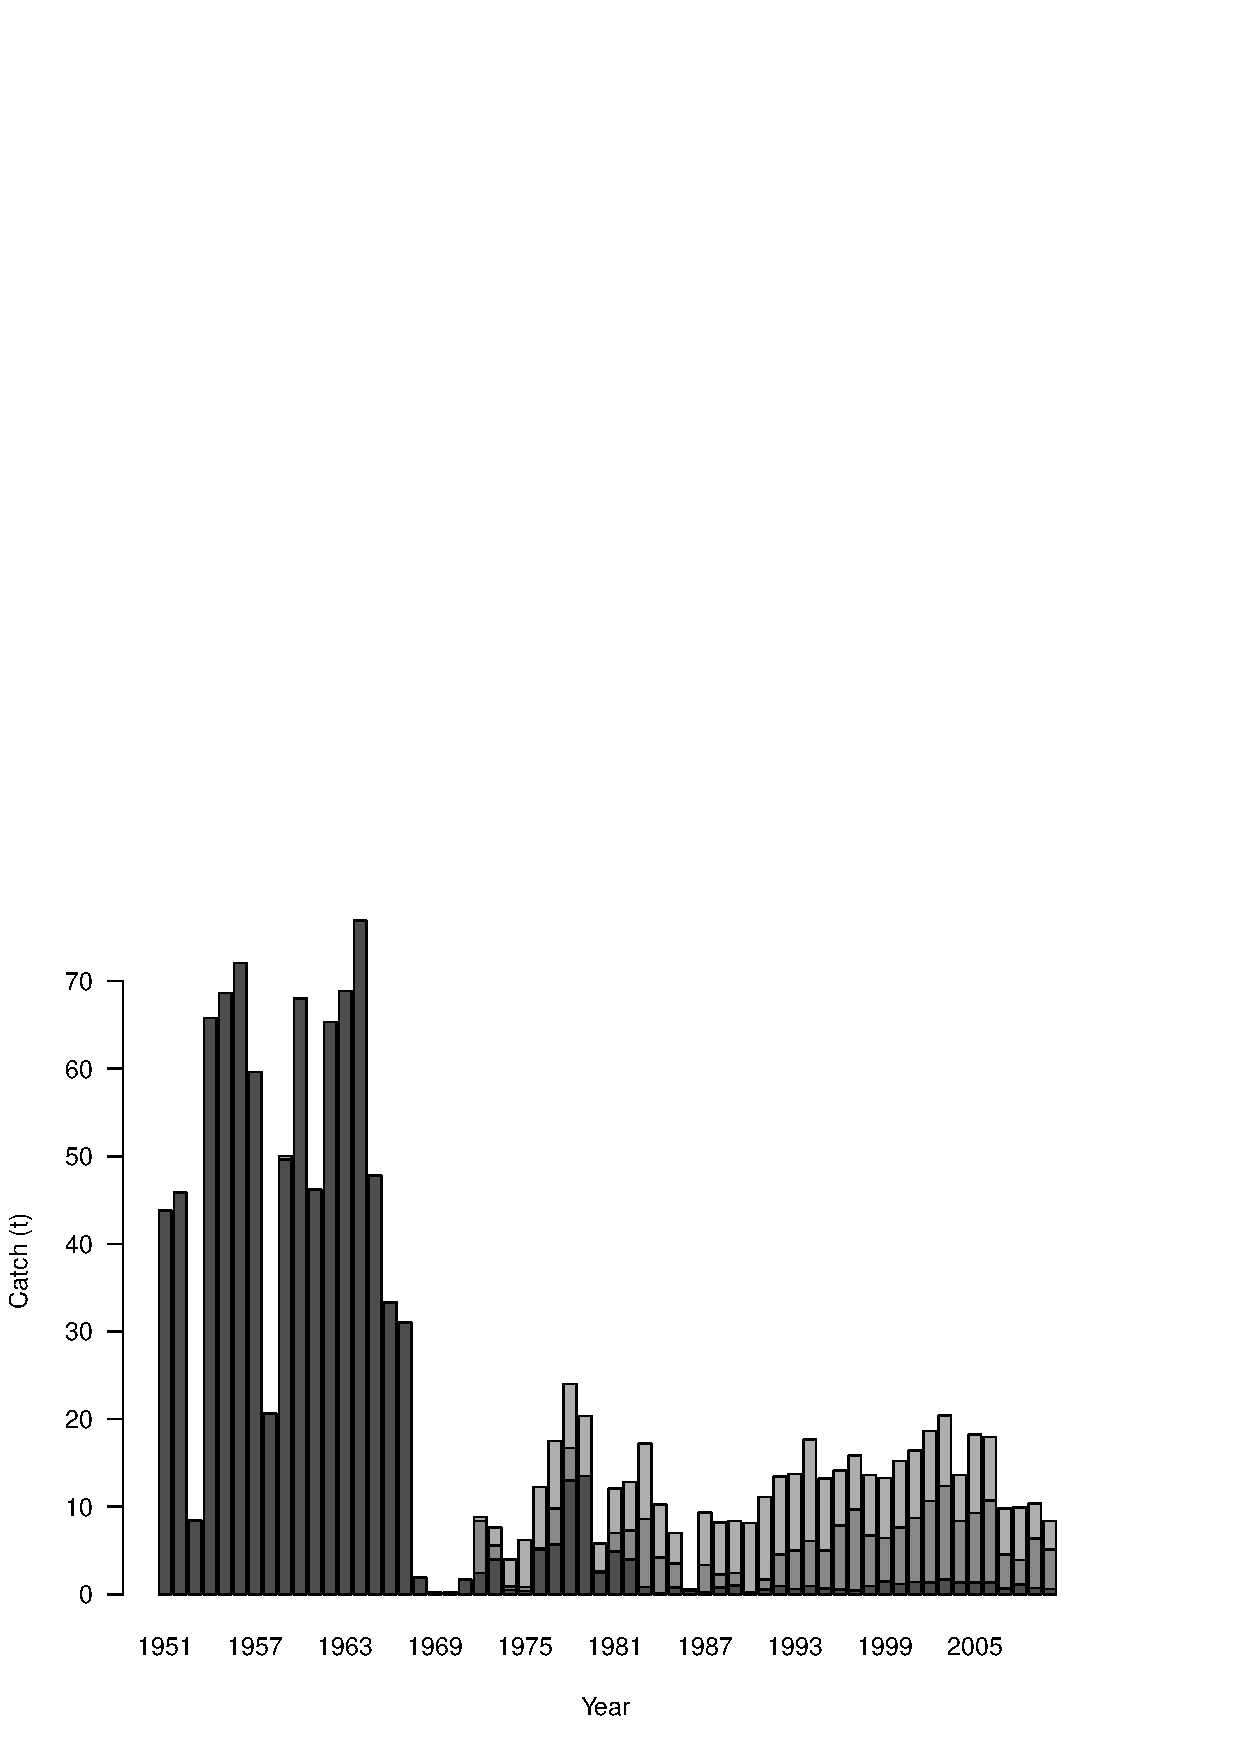
\includegraphics[width=\columnwidth]{iscamfigs/pHerringFig1.pdf}\\
% 	\caption{Total landings of Pacific herring in the Strait of Georgia stock assessment region by purse-seine (dark bars), Sn-roe (medium) and gill net (light bars).}\label{pHerringFig1}
% \end{figurehere}
% 
% 
% \subsection{Data \& control files}
% The available data for the herring fishery consist of commercial landings for each of the three fisheries, age-composition data from each of these fisheries (see Figure \ref{pHerringFig3} for the winter purse seine fishery), average weight-at-age of the catch, and a fisheries independent spawning biomass index (based on spawn deposition).  The spawn survey index is split into two separate series that correspond to a change in methods for estimating spawning deposition between 1987 and 1988.  The model is fit to all of these data and uses the empirical weight-at-age data to convert numbers-at-age to biomass.
% 
% 
% 
% 
% In this example, the command line option \texttt{-sim 000} is invoked to simulate fake data based on parameter values specified in the control file.  Recall the command line option \texttt{-sim} is used to tell \iscam\ to overwrite the existing observations in memory with simulated values (in this case with zero error because the random number seed is set to 000), and then attempt to estimate these model parameters.  If all is working correctly, the \texttt{iscam.par} file should have nearly identical estimates for the model parameters as the initial values that are specified in the control file.
% 
% The control file used in this example is shown here, and there are a couple of things that should be highlighted with simulating data with no error.  First off, the phase for the variance and variance partitioning parameters ($\vartheta$ and $\rho$, respectively) should be set to a negative value and not be estimated.  Second ensure that the upper bound for $\vartheta$ (vartheta or the total precision) is set to a very high value (say 5000) and the initial value is set close to the upper bound (4999 in this case).  The reason for fixing the parameters should be obvious, there is no error in the data to begin and thus its not necessary to estimate the total variance.  The reason to set the initial value of $\vartheta$ to a large value is to minimize the a slight bias due to the lognormal bias correction in the stock-recruitment relationship (i.e., the $-0.5\tau^2$ in \ref{T4.12} or \ref{T4.13}) during the parameter estimation phase.  If you do not specify a large value of $\vartheta$ then it is unlikely that you will obtain nearly exact estimates of the unfished recruitment $R_o$.
% 
% 
% %%Here is a pdf figure rotated.
% \begin{figurehere}
% 	% Requires \usepackage{graphicx}
% 	\centering
% 	%\psfrag{Year}[][c]{Year}
% 	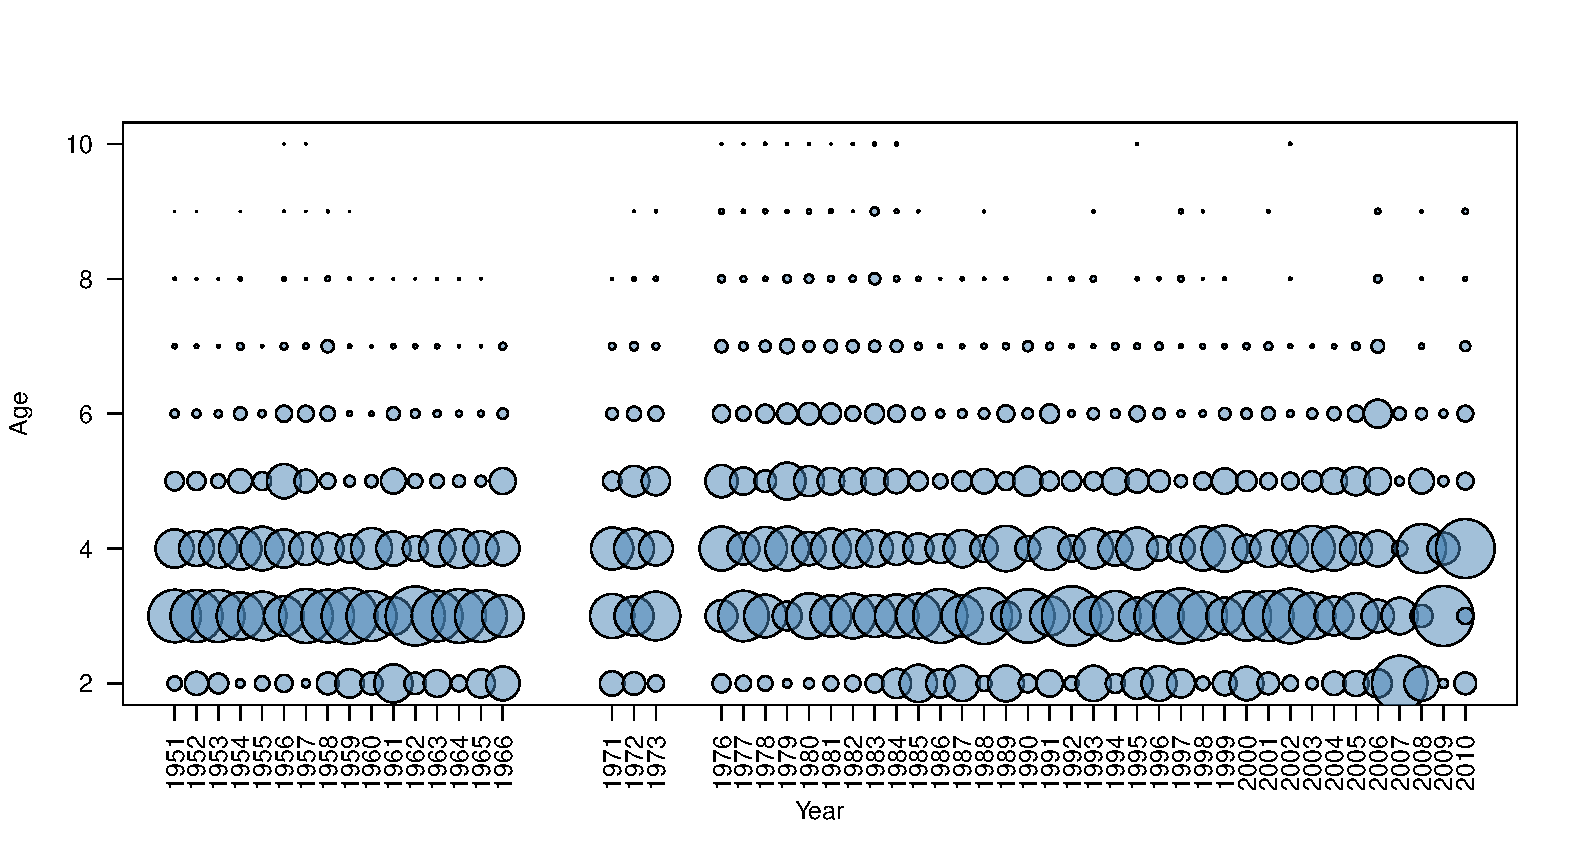
\includegraphics[height=\columnwidth,angle=-90]{iscamfigs/pHerringFig3.pdf}\\
% 	\caption{Age comps for the purse seine fishery in the Strait of Georgia between 1951 and 2010.}\label{pHerringFig3}
% \end{figurehere}
% \vspace{0.1in}
% 
% \noindent \hrulefill\\
% \small
% Control file for the SOG herring example
% \tiny
% \begin{alltt}
% \input{../../../Examples/sogHerring/SOGHerring2010sim.ctl}
% \end{alltt}
% \hrulefill
% \normalsize
% 
% 
% \subsection{Results}
% The ability of the model to estimate the parameters is demonstrated by the estimates of spawning stock biomass and the estimated fishing mortality rates for each of the fisheries.  Shown in Figure \ref{pHerringFig2} is the estimated pre-fishery biomass and the spawning stock biomass for the simulated data where the true values for the spawning stock biomass are shown by the filled circles.  Estimates of spawning stock biomass exactly match the true values that were used to simulate the data.  Departures from the true values when there is no simulated error would imply a structural problem, or potential coding error, and should be investigated further before proceeding with an actual assessment.
% 
% 
% \begin{figurehere}
% 	% Requires \usepackage{graphicx}
% 	\psfrag{Year}[][c]{Year}
% 	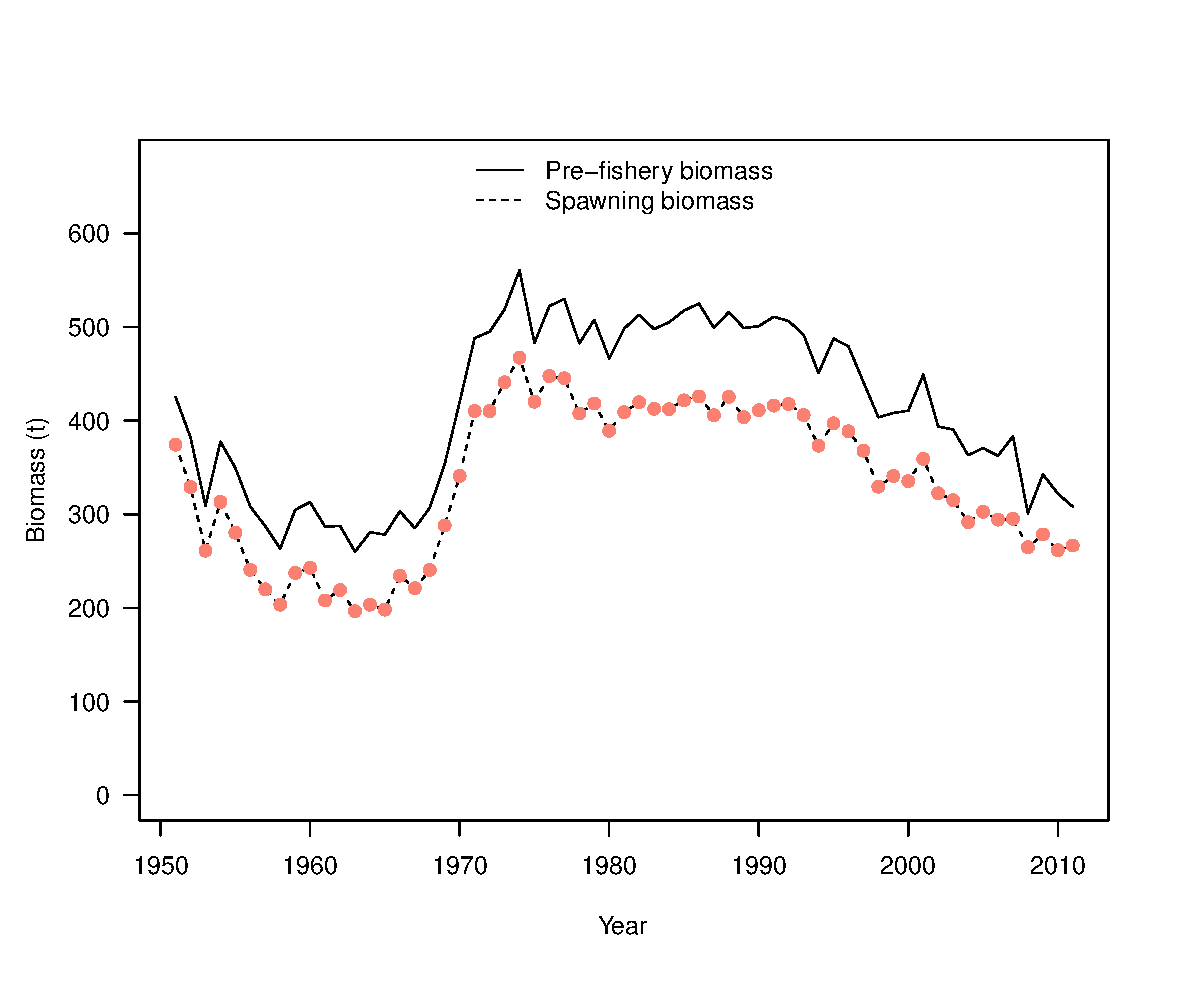
\includegraphics[width=\columnwidth]{iscamfigs/pHerringFig2.eps}\\
% 	\caption{Estimates of pre-fishery biomass and spawning stock biomass (lines) from \iscam\  in comparison to the true spawning stock biomass (filled points) based on the simulation model. No errors were generated in the simulation model.}\label{pHerringFig2}
% \end{figurehere}
% 
% 
% 
% \end{multicols}
% 




%%%%%%%%%%%%%%%%%%%%%%%%%%%%%%%%%%%%%%%%%%%%%%%%%%%%
%%%%%%%%%%%%%%%%%%%%%%%%%%%%%%%%%%%%%%%%%%%%%%%%%%%%
%%%%%%%%%%%%%%%%%%%%%%%%%%%%%%%%%%%%%%%%%%%%%%%%%%%%


\section{Example Assessment: the Namibian hake case study}
\begin{multicols}{2}
As a simple example of fitting \iscam\ to CPUE data only, we use the Namibian hake case study from chapter 10 in the Ecological Detective \citep{hilborn1997ecological}.  In this example the available data consist of catch (thousands of tons) and CPUE (tons per standardized trawl hour).  \cite{hilborn1997ecological} provide three alternative models to the data that range from simple 4 parameter Schaefer production models (observation \& process error only) and a 5 parameter lagged recruitment, growth/survival model.  In this example they assume the stock is at an unfished state in 1967.

To conduct the assessment using \iscam\ with the same unfished assumption in 1965, the 			``Assume unfished in first year (0=FALSE, 1=TRUE)'' flag must be set to 1 (see the following control file). \iscam\ is an age-structured model, and in this example there are no available age-composition data to compare with. Therefore we must also assume a selectivity curve for this fishery.  In this example, selectivity was assume to follow a logistic function with the 50\% vulnerability-at-age equal to 3.5 years with a standard deviation of  1.0 years.  It is also necessary in this case to turn off the estimation of the selectivity parameters by setting the estimation phase to a negative number (e.g., -1).  

For the estimated leading parameters, two of the six parameters are not estimated \verb"#log_m" and \verb"#rho", which is the instantaneous natural mortality rate and the proportion of the total error that is associated with observation errors.  A bounded uniform prior is assumed for $R_o$ and a beta prior for steepness $h$ with an expected value of 0.6.  The natural mortality rate $M$ is assumed known and fixed at a value of 0.345.  A uniform bounded prior is assumed for the log of the average recruitment level, and a non-informative gamma prior is assumed for the total precision $\kappa$.  In this example we assume that the total error is allocated to observation and process error equally ($\rho= 0.5$).

\tiny
\noindent \hrulefill
\begin{alltt}
Control file for the Namibian hake data.
\input{../../../examples/ECODETECTIVE/Data/NamibianHake.ctl}
\end{alltt}
\hrulefill
\normalsize

To convert numbers-at-age to biomass, growth was based on the von Bertalanffy growth parameters in the \verb"NamibianHake.dat" file and the allometric relationship $w_a=a(l_a)^b$. Maturity-at-age is  based on the logistic function with age-4 being the age at 50\% maturity and 0.2 is the standard deviation. The plus group age was assumed to be 25 years, and there is only one fishing gear exploiting this stock.

Catch is taken by a single gear each year between 1965 and 1987, and the relative abundance index is based on the catch per standardized hour of trawling for the commercial gear.  It is assumed that each CPUE observation is assumed to have the same error distribution, and the relative weights of each observations are all set equal to one.

There is no age-composition data to speak of, but \verb"#na_gears" must have a value of 1 in order to proceed with reading the remaining portion of the data file.

\tiny
\noindent \hrulefill
\begin{alltt}
Data file for the Namibian hake data.
\input{../../../examples/ECODETECTIVE/DATA/NamibianHake.dat}
\end{alltt}
\hrulefill
\normalsize

%%Results for Namibian hake.
\subsection{Maximum likelihood estimates of the model parameters}
Estimates of unfished spawning biomass is 2,877, steepness is 0.79, MSY is 266, and \fmsy is 0.33.  These results are  very similar to those obtained by \cite{hilborn1997ecological} for the Schaefer model with observation error.  Estimates of the total standard deviation amount to 0.16 which equally breaks down to 0.081 for observation and process errors.

\begin{figurehere}
	\centering
	\includegraphics[width=0.9\columnwidth]{iscamFigs/NhakeFigs.eps}
	\caption{Estimates of total biomass and spawning biomass, observed and predicted CPUE, for the Namibian hake data from \iscam. Unfished biomass, \bmsy, and MSY based depletion levels are shown as horizontal dotted lines.}\label{fig4}
\end{figurehere}

\subsection{Bayesian analysis of model parameters \& policy parameters}
Marginal posterior distributions of model parameters were constructed by using the metropolis algorithm built into ADMB to sample from the joint posterior distribution.  This is accomplished by running \iscam\ in -mcmc mode followed by the -mceval option to produce the \verb"iscam.mcmc" output file.  In this example an MCMC chain of length 1,000,000 was run and samples were taken systematically every 500 iterations (\verb"-mcsave 500"), which results in a posterior sample size of 2000.

Uniform prior distributions for the unfished recruitment and average recruitment ($R_0$ and $\bar{R}$), and non-informative gamma prior for the precision parameter ($1/\vartheta$).  In the case of the steepness parameter, a non-informative beta prior was used ($p(h)\sim beta[1.01,1.01]$), where steepness is re-scaled to the interval 0.2-1.0 (i.e, $(h-0.2)/0.8$) such that a 0 probability was assigned for $h$ values less than 0.2.  In comparison to the results obtained by \cite{hilborn1997ecological} using a biomass production model with lagged recruitment and a Beverton-Holt recruitment function, the data here appear to have some information about the steepness parameter (Fig. \ref{fig5}).  This owes in part to differences in assumptions about growth, maturity and selectivity between the LRGS model used by \cite{hilborn1997ecological} and this \iscam\ example.

\begin{figurehere}
	% Requires \usepackage{graphicx}
	\centering
	% \psfrag{log.ro}[c][][0.75]{$\ln(R_0)$}
	% 	\psfrag{log.rbar}[c][][0.75]{$\ln(\bar{R})$}
	% 	\psfrag{kappa}[c][][0.75]{$\vartheta$}
	% 	\psfrag{h}[c][][0.75]{$h$}
	%%\includegraphics[width=\columnwidth]{iscamFigs/fig5.eps}\\
	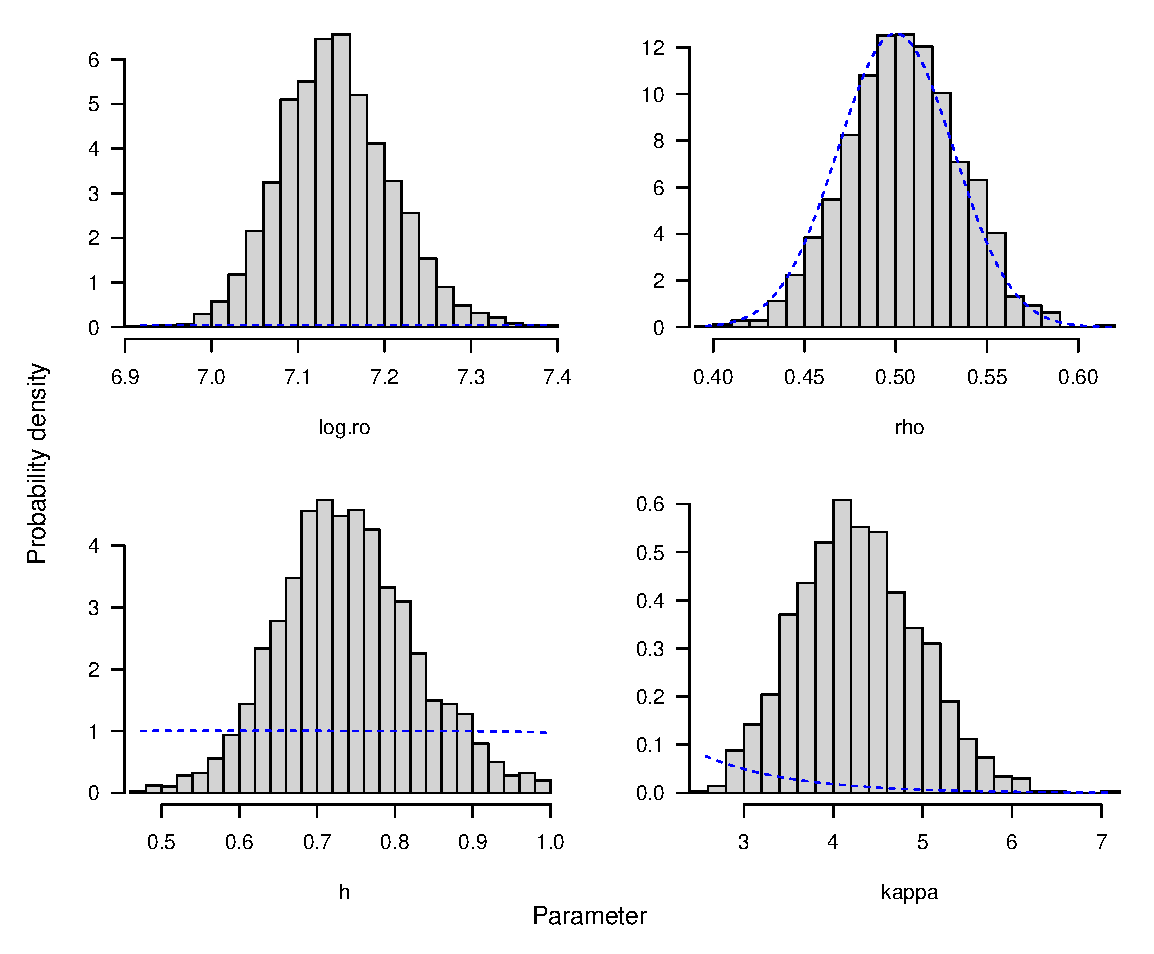
\includegraphics[width=0.9\columnwidth]{iscamFigs/nHakeparameters.pdf}\\
	\caption{Marginal posterior probability densities (histograms) and prior densities (lines) for unfished recruitment $R_0$, steepness $h$, mean recruitment $\bar{R}$ and recruitment compensation $\kappa$ for the Namibian hake case study.}\label{fig5}
\end{figurehere}

Marginal posterior densities can also be produced for derived quantities such as MSY based reference points (Fig \ref{fig6}).   Again, although not directly comparable due to structural differences between \iscam\ and the LRGS model, the marginal posterior distributions for MSY and $B_0$ are very similar.  More importantly however is that these marginal distributions can also be used to calculate the probability that the stock is currently overfished and if overfishing is occurring.  This is normally represented from a maximum likelihood perspective where the trends in biomass relative to \bmsy and fishing mortality rates relative to \fmsy are plotted against each other (these are known as KOBE plots, Fig \ref{fig7}).

\begin{figurehere}
	% Requires \usepackage{graphicx}
	\centering
	% \psfrag{bo}[c][][0.75]{$B_0$}
	% 	\psfrag{bmsy}[c][][0.75]{\bmsy}
	% 	\psfrag{msy}[c][][0.75]{MSY}
	% 	\psfrag{fmsy}[c][][0.75]{\fmsy}
	%%\includegraphics[width=\columnwidth]{iscamFigs/fig6.eps}\\
	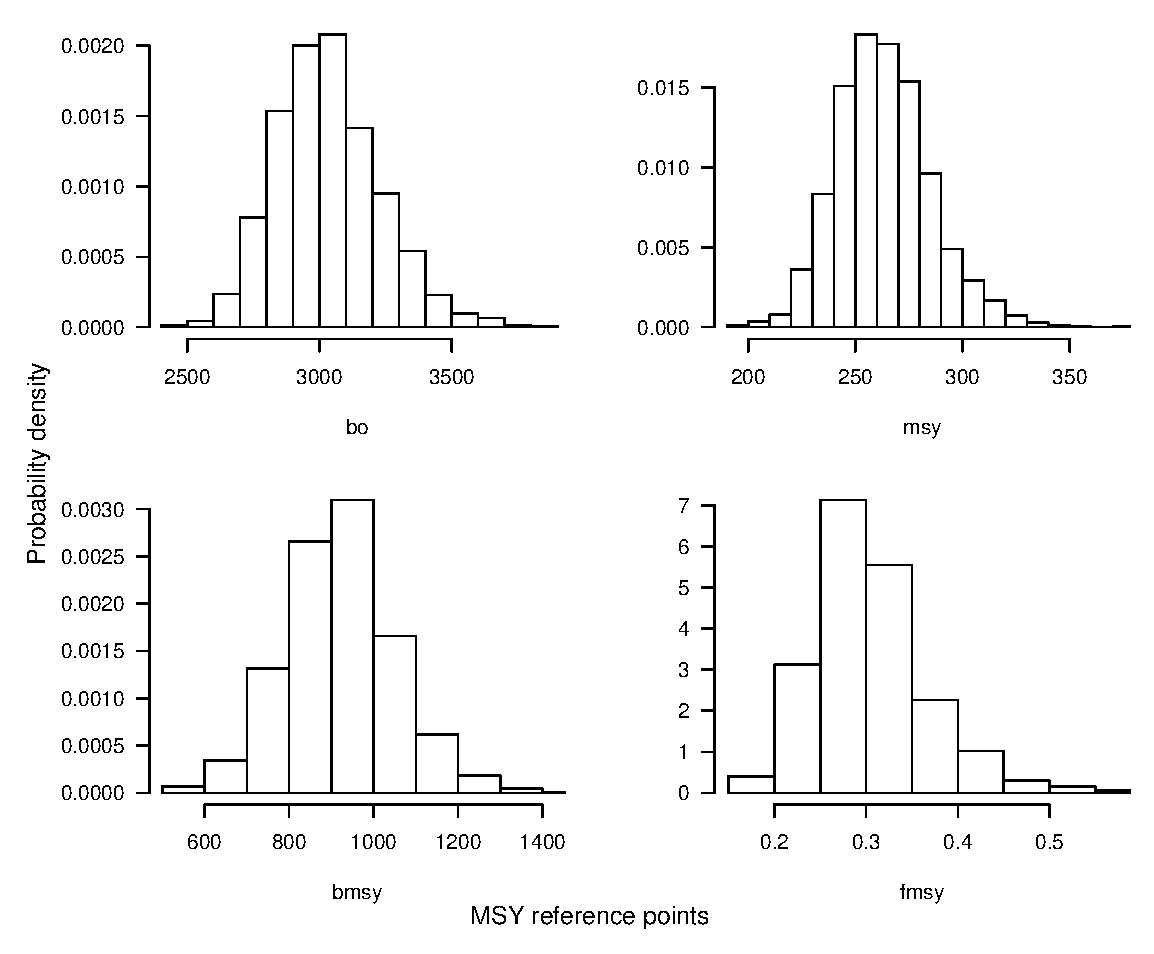
\includegraphics[width=0.9\columnwidth]{iscamFigs/nHakerefpoints.pdf}\\
	\caption{Marginal posterior probability densities for unfished spawning biomass $B_0$, optimal spawning biomass \bmsy, MSY and \fmsy\ for the Namibian hake case study.}\label{fig6}
\end{figurehere}

To represent changes in stock status over time, the default plot compares estimates of spawning stock biomass relative to the estimates of \bmsy versus fishing mortality rates relative to \fmsy.  Uncertainty in stock status for the last year is based on the joint posterior distribution and a credible interval is given by a contour plot that represents a `fried egg'.

\begin{figurehere}
	\centering
	% \psfrag{bstatus}[c][][0.75]{$B_t/$\bmsy}
	% 	\psfrag{fstatus}[c][][0.75]{$F_t/$\fmsy}
	%%\includegraphics[width=\columnwidth]{iscamFigs/fig7.eps}\\
	\includegraphics[width=0.9\columnwidth]{iscamFigs/NhakeKobeplot.pdf}\\
	\caption{Stock status plot (or Kobe plot) where the ``fried egg'' represents uncertainty.}\label{fig7}
\end{figurehere}

\end{multicols}



%%%%%%%%%%%%%%%%%%%%%%%%%%%%%%%%%%%%%%%%%%%%%%%%%%%%
%%%%%%%%%%%%%%%%%%%%%%%%%%%%%%%%%%%%%%%%%%%%%%%%%%%%
%%%%%%%%%%%%%%%%%%%%%%%%%%%%%%%%%%%%%%%%%%%%%%%%%%%%
\section{Example Assessment: the Pacific hake fishery}
\begin{multicols}{2}
\subsection{Data \& assumptions}
As more complex example assessment, the data from the Pacific hake fishery is used.  Pacific hake (\textit{Merluccius productus})  in the Northeast Pacific has a migratory coastal stock that is harvested by US and Canadian fishing fleets during the summer and late fall.  This data is an extension to the previous work in \cite{Martell2008pam}.  In this example the data has been restricted to the years 1977-2009, as this was a period when catch-age data from both the Canadian and US fisheries was available and could be aggregated using a weighted average based on the catch proportion from each nation.

The data from this fishery consists of a combined total catch, a relative abundance index from an acoustic survey conducted on a triannual and biannual basis, age-composition data from the commercial fishery, and finally age-composition data from the acoustic trawl survey. The coastal Pacific hake stock undergo an annual migration from spawning grounds in the south near Baja California Sur in the winter to summer feeding grounds to the north; the extent of the northward migration is highly variable and ranges from Oregon--Washington to Southeast Alaska in some years.  Larger/older fish tend to migrate further north.  Inter-annual variation in the extent of the migration leads to variation in selectivity to the fishery.  To accommodate the time-varying selectivity, a total of 85 nodes for a bicubic spline are estimated (17 nodes for the year effect, and 5 nodes for the age effect, see Fig. \ref{Fig3}).

\begin{figurehere}
	\centering
	\includegraphics[width=0.8\columnwidth]{iscamFigs/phakefig15.eps}\\
	\caption{Combined observed landing from the US and CAN fisheries for Pacific hake between 1977 and 2009.}\label{fig8}
\end{figurehere}

In this example it was assumed that recruitment follows a Beverton-Holt relationship, the stock is not at its unfished state in 1977, natural mortality is independent of age and constant over time, and survey selectivity is asymptotic and time-invariant.  


Here is the \iscam\ control file for the Pacific hake data, and the data file is provided at the end of this section on page \pageref{HakeDataFile}.  The observed combined landings from both the US and Canadian zones have averaged about 233,000 metric tons between 1977 and 2009, and in the last 10 years has averaged 270,000 mt with a peak in 1994 of 361,000 mt  (Fig. \ref{fig8}.)\\
\tiny
\noindent \hrulefill
\begin{alltt}
\input{../../../examples/PacificHake/Data/2010/PHake2010.ctl}
\end{alltt}
\hrulefill
\normalsize


%
%\begin{figurehere}
%	\centering
%	\includegraphics[width=0.4\columnwidth]{iscamFigs/phakefig1.eps}\\
%	\caption{Assumed age-schedule information for this example assessment.}\label{fig8b}
%\end{figurehere}


\subsection{Maximum likelihood estimates}
A total of 176 model parameters were estimated and it took  roughly 10 seconds to obtain maximum likelihood estimates, including the calculations for the Hessian matrix on a MacBook Pro, with a 2.66 GHz Intel Core i7 processor.

Maximum likelihood estimates of total biomass and spawning biomass along with estimates of $B_0$ and \bmsy are shown in Fig. \ref{fig9}.  Starting in 1977, estimates of spawning biomass was just slightly less than the estimate of \bmsy.  Starting in the 1980's, spawning biomass increased to a maximum in 1990 owing to two very large year classes (1980 and 1984, Fig. \ref{fig10}). Between 1985 and 1999, recruitment ranged between average and median values and the spawning stock biomass declined to less than \bmsy values in 2001 while fisheries removals exceeded 200,000 mt per year.  Another significant year class (1999) was responsible for rebuilding the spawning stock biomass up to 2004, and since 2005, the spawning stock biomass has continued to decline.

Information to estimate age-1 recruitment for Pacific hake comes from the catch-age composition data.  Between 1978 and 2009 the average age-1 recruitment is estimated to be 2.72 billion individuals and the median value is 1.16 billion individuals (Fig. \ref{fig11}).  The maximum likelihood estimate of the standard deviation in recruitment ($\tau$, see eq. \ref{T4.2} on page \pageref{tab:statistical_catch_age_model}) was 1.29 given the prior information specified in the control file for this assessment.


\begin{figurehere}
	\centering
	\includegraphics[width=0.9\columnwidth]{iscamFigs/phakefig2.eps}\\
	\caption{Maximum likelihood estimates of total biomass and spawning stock biomass for Pacific hake along with reference points (dotted lines) for unfished spawning biomass $B_0$ and \bmsy.}\label{fig9}
\end{figurehere}


\begin{figurehere}
	\centering
	\includegraphics[width=0.9\columnwidth]{iscamFigs/phakefig14.eps}\\
	\caption{Maximum likelihood estimates of age-1 recruits from 1978 to 2009, with median and average values shown as the horizontal dashed and dotted lines.}\label{fig10}
\end{figurehere}

Current estimates of stock status relative to \bmsy\ and the removal rate relative to \fmsy is estimated to be in the critical zone in term of the Department of Fisheries and Oceans Canada, Fisheries Management Framework (Fig. \ref{fig11}).  Estimates of the spawning stock biomass are less than 80\% of \bmsy and are currently in the cautious zone.  Estimates of fishing mortality rate are roughly 1.5 times the estimate of \fmsy.  Maximum likelihood estimates of \bmsy and \fmsy are 1.13 million mt 0.336, respectively. 

\begin{figurehere}
	\centering
	\includegraphics[width=0.9\columnwidth]{iscamFigs/phakefig8.eps}\\
	\caption{Maximum likelihood estimates of stock status ($B_t/$\bmsy) and removal rate ($F_t/$\fmsy) for Pacific hake relative to the Department of Fisheries and Oceans Canada's  Fisheries Management Framework.}\label{fig11}
\end{figurehere}

Model fit can be partially judged by the residual patterns between the observed and predicted data (Fig. \ref{fig12}).  The catch data are assumed to be measured fairly accurately with a small standard deviation ($\sigma_C=0.025$) in measurement errors; the largest residual in the catch is just less than 100 mt in 1981.  

Recall that \iscam\ directly estimates annual recruitment values, and the reported residuals in Fig. \ref{fig12} correspond to the log differences between the estimated recruitment and a Beverton-Holt model prediction where $R_0$ and steepness $h$ are the estimated parameters for the stock recruitment model.  The strong 1980, 1984 and 1999 cohorts, show up as strong positive residuals in 1981, 1985 and 2000 in the residual plot (note that the age-at-recruitment is 1 year).  The 2002 and 2004 cohorts appear to be well below the median values in recent years, and the 2005 cohort is currently estimated to be the next largest cohort since 1999.

\begin{figurehere}
	\centering
	\includegraphics[width=0.9\columnwidth]{iscamFigs/phakefig11.eps}\\
	\caption{Residuals between the observed and predicted catch, deviations between estimated recruitment and a deterministic Beverton-Holt model, and the observed and predicted relative abundance data from the acoustic survey.}\label{fig12}
\end{figurehere}


\subsection{Time-varying selectivity}
Estimates of time-varying selectivity for the commercial fishery were based on estimating 85 nodes (17 years and 5 ages) and interpolating between these nodes using a bicubic spline.  The estimated nodes in \iscam\ are equidistant, and the total number of estimated nodes is specified in the control file.  Increasing the number of estimated nodes should improve the overall fit to the age-composition data; however, this comes at the expense of increasing the associated uncertainty in overall model parameter estimates.  To ensure that the model is not over-fitting the data, there are two additional penalties that are added to the objective function that limit the rate of change in age-effects (penalty weight for second differences), and how much dome-shaped is allowed in the age-effects.  Increasing the penalty weight on second differences insures a smoothed increase or decrease in the selectivity-at-age, and increasing the weight on the dome-shaped penalty reduces the amount of dome-shaped selectivity that can occur.  Again, these penalty weights are specified in the control file  in the selectivity parameters section.

In the Pacific hake example, estimates of selectivity increase with age during the late 1970s and early 1980s (Fig. \ref{fig13}).  As the 1980 and 1984 cohorts recruit to the fishery, the selectivity shifts to younger ages, and becomes more dome-shaped.  At the peak of the spawning stock biomass in 1990, selectivity increases continuously with age, and is more or less asymptotic until the 1999 cohort enters the fishery.  Recent estimates of selectivity indicate that the 1999 cohort (age-10 in the year 2009) is still strongly selected for, but as the biomass of the 1999 cohort erodes there is an apparent increase in selectivity for older ages (Fig. \ref{fig13}).

\begin{figurehere}
	\centering
	\includegraphics[width=0.9\columnwidth]{iscamFigs/phakefig9a.eps}\\
	\caption{Estimates of selectivity for the commercial fishery.}\label{fig13}
\end{figurehere}


\begin{figurehere}
	\centering
	\includegraphics[width=0.9\columnwidth]{iscamFigs/phakefig13a.eps}\\
	\caption{Observed age-composition (top panel) and Pearson residuals between observed and predicted proportions-at-age in the commercial fishery (bottom panel, with negative residuals given by dark circles).}\label{fig13a}
\end{figurehere}

The residual patterns in the age composition data from the commercial fishery don't appear to have any significant pattern that would indicate a major model mis-specification (Fig. \ref{fig13a}).  There is a tendency for age-2 proportions to have more negative residuals and age-3 positive residuals, but over all these residuals are fairly small.  This is not much of a surprise given the flexibility of the time-varying selectivity that was assumed in the commercial fishery.


Although not shown here, the residual pattern for the survey age composition also appears to be random, and in this case a time-invariant asymptotic selectivity curve was used for the acoustic survey. Survey data from 1995 to 2007 were assumed to be twice as accurate in comparison to the data collected prior to 1995 when spatial coverage of the survey was incomplete.  Also, the 2009 survey carries no weight as this survey was contaminated by the presence of Humboldt squid (\textit{Dosidicus gigas}) during the 2009 survey.  Additional details about the data for the Pacific hake assessment and the methods used to aggregate the age-composition for the US and CAN fisheries can be found in \cite{Martell2009}.

\subsection{Bayesian implementation}
To obtain samples from the joint posterior distribution and obtain median values and credible intervals, \iscam\ was run using the Metropolis-Hastings routine that is built into ADMB.  In this example, 2000 systematic samples from a chain of length 1,000,000 was used.  The total runtime for conducting a MCMC sample  of length 1,000,000 was 39 minutes and 56 seconds with 176 estimated parameters.

The marginal posterior distributions and the corresponding prior distributions are shown in Fig. \ref{fig14}.  There is no information in the data about the underlying steepness of the stock recruitment relationship; this is clearly shown by the marginal posterior distribution for $h$ reflects the assumed (\emph{ad hoc}) prior distribution.

\begin{figurehere}
	\centering
	% \psfrag{log.ro}[c][][0.5]{$\ln(R_0)$}
	% \psfrag{log.rbar}[c][][0.5]{$\ln(\bar{R})$}
	% \psfrag{h}[c][][0.5]{$h$}
	% \psfrag{rho}[c][][0.5]{$\rho$}
	% \psfrag{log.m}[c][][0.5]{$\ln(M)$}
	% \psfrag{kappa}[c][][0.5]{$\vartheta$}
	\includegraphics[width=0.9\columnwidth]{iscamFigs/phakefig5.eps}\\
	\caption{Marginal posterior densities and prior densities for the leading parameters in \iscam.}\label{fig14}
\end{figurehere}

The prior distributions for each of the estimated leading parameters are specified in the control file.  In this example, a normal prior was assumed for the unfished recruitment ($\ln(R_0)$) and the log of the natural mortality rate ($\ln(M)$), a beta prior for the steepness ($h$) and the fraction of the total error that is associated with observation error ($\rho$), and a non-informative gamma prior for the total precision ($\vartheta$).  A uniform prior was specified for the average recruitment ($\ln(\bar{R})$).

Recent trends in the spawning stock biomass, and depletion, along with the associated uncertainty in the form of a credible interval are given in Table \ref{iscam.T1}.  Projected estimates of spawning stock depletion at the start of 2010 is 22\%, with a lower bound of 7.5\% and an upper bound of 53.2\%.  This translates into a projected spawning stock biomass of 670,000 mt with a 95\% credible interval of 255,000 mt to 1,506,000 mt.

\begin{tiny}
% latex.default(tail(t1, 10), file = filename, rowname = NULL,      caption = cap, cgroup = cgrp, n.cgroup = ncgrp, label = "iscam.T1") 
%
\begin{table}[!tbp]
 \caption{Recent trends in median estimate and 2.5\% and 97.5\% 
					credible intervals for spawning stock biomass, and
					spawning stock depletion. These estimates are based 
					on sampling the joint posterior distribution using MCMC.\label{iscam.T1}} 
 \begin{center}
 \begin{tabular}{rcrrrcrrr}\hline\hline
\multicolumn{1}{c}{\bfseries  }&
\multicolumn{1}{c}{\bfseries }&
\multicolumn{3}{c}{\bfseries Spawning stock biomass}&
\multicolumn{1}{c}{\bfseries }&
\multicolumn{3}{c}{\bfseries Depletion}
\tabularnewline \cline{1-9}
\multicolumn{1}{c}{Year}&\multicolumn{1}{c}{}&\multicolumn{1}{c}{2.5\%}&\multicolumn{1}{c}{median}&\multicolumn{1}{c}{97.5\%}&\multicolumn{1}{c}{}&\multicolumn{1}{c}{2.5\%}&\multicolumn{1}{c}{median}&\multicolumn{1}{c}{97.5\%}\tabularnewline
\hline
$2001$&&$0.877$&$1.012$&$1.226$&&$0.125$&$0.264$&$0.468$\tabularnewline
$2002$&&$1.043$&$1.217$&$1.554$&&$0.147$&$0.319$&$0.571$\tabularnewline
$2003$&&$1.874$&$2.200$&$2.945$&&$0.270$&$0.578$&$1.058$\tabularnewline
$2004$&&$2.017$&$2.395$&$3.306$&&$0.290$&$0.629$&$1.169$\tabularnewline
$2005$&&$1.692$&$2.048$&$2.976$&&$0.249$&$0.537$&$1.024$\tabularnewline
$2006$&&$1.242$&$1.569$&$2.450$&&$0.187$&$0.414$&$0.803$\tabularnewline
$2007$&&$0.851$&$1.174$&$2.053$&&$0.137$&$0.309$&$0.630$\tabularnewline
$2008$&&$0.543$&$0.886$&$1.815$&&$0.096$&$0.234$&$0.537$\tabularnewline
$2009$&&$0.312$&$0.780$&$2.099$&&$0.061$&$0.200$&$0.593$\tabularnewline
$2010$&&$0.169$&$0.726$&$2.280$&&$0.036$&$0.188$&$0.637$\tabularnewline
\hline
\end{tabular}

\end{center}

\end{table}


\end{tiny}

Relative to the spawning stock depletion reference points, the median estimate of spawning stock biomass falls in the critical zone (Fig. \ref{fig16}).  Estimates of spawn stock depletion is very uncertain; there is a fairly high probability that the stock is also in the critical zone, or less than 40\% of \bmsy.

\begin{figurehere}
	\centering
	\includegraphics[width=0.9\columnwidth]{iscamFigs/phakefig12.eps}\\
	\caption{Median estimates of spawning stock depletion and 95\% credible interval based 2000 samples from the joint posterior distribution. Transition between the critical, cautious and healthy zones is defined as 0.4\bmsy/$B_0$ and 0.8\bmsy/$B_0$, respectively }\label{fig16}
\end{figurehere}

\begin{scriptsize}
% latex.default(t1, "", file = filename, caption = cap, label = "iscam.T2") 
%
\begin{tablehere}
 \caption{Maximum likelihood estimates (MLE) and standard deviations (SD)
				based on the inverse Hessian for the six leading parameters. Median
				values and the 95\% credible interval based on posterior samples.\label{iscam.T2}} 
 \begin{center}
 \begin{tabular}{lrrrrr}\hline\hline
\multicolumn{1}{l}{}&\multicolumn{1}{c}{MLE}&\multicolumn{1}{c}{SD}&\multicolumn{1}{c}{Median}&\multicolumn{1}{c}{2.5\%}&\multicolumn{1}{c}{97.5\%}\tabularnewline
\hline
$\ln(R_0)$&$ 1.167$&$0.326$&$ 1.238$&$ 0.674$&$ 1.958$\tabularnewline
$h$&$ 0.688$&$0.214$&$ 0.669$&$ 0.370$&$ 0.932$\tabularnewline
$\ln(M)$&$-1.478$&$0.049$&$-1.457$&$-1.554$&$-1.363$\tabularnewline
$\ln(\bar{R})$&$-0.168$&$0.119$&$-0.103$&$-0.343$&$ 0.177$\tabularnewline
$\rho$&$ 0.293$&$0.043$&$ 0.305$&$ 0.227$&$ 0.405$\tabularnewline
$\vartheta$&$ 0.525$&$0.053$&$ 0.517$&$ 0.422$&$ 0.623$\tabularnewline
\hline
\end{tabular}

\end{center}

\end{tablehere}


\end{scriptsize}

\end{multicols}




Here is the data file for \iscam.
\tiny
\begin{alltt}
  \input{../../../examples/PacificHake/DATA/2010/PHake2010.dat}\label{HakeDataFile}
\end{alltt}
\normalsize




%    %!TEX root = /Users/stevenmartell/Documents/CURRENT PROJECTS/iSCAM-trunk/fba/BC-herring-2011/WRITEUP/BCHerring2011.tex
\section{Methods}
	\subsection{Input data \& assumptions}
	\subsubsection{Catch data}
	For each of the statistical areas, the required input data for \iscam\ consists of a catch time series for each of the fishing fleets.  For the BC herring fishery, the annual total removals has been partitioned into three distinct fishing fleets (or fishing periods, see Figure \ref{FigCatch}).  The first fleet is a winter seine fishery that has been in operation since the start of the assessment in 1951, the second is a seine-roe fishery that commenced in 1972 in the Strait of Georgia, and the third fleet is a gillnet fishery that targets females on the spawning grounds. The model is fit to the catch time series information and assumes measurement errors are lognormal, independent and identically distributed.  The assumed standard deviation in the catch observations must be specified in the control file and it is assumed that measurement errors in the catch is the same for all fishing periods.  The units of the catch are given in 1000s of metric tons.
	
	In addition to the commercial catch, removals from fisheries independent surveys must also be specified in \iscam. Two additional fleets are specified to represent the spawn survey, where the spawn survey is broken into two distinct time periods pre-1988 and post-1988, the year when the survey switched from surface surveys to dive surveys.  This partitioning of the data is done for two reasons: (1) to allow for different catchability coefficients to be specified for the early and late periods, and to allow for more weight to be placed on the contemporary data due to improved precision in the estimates of egg layers. 

%TODO decide if the test fishery data is going to be looked at here or in the appendix
	In the case where the test fishery data has been separated from the seine roe fishery, an additional fleet is specified in the data file and fishing mortality rates for the test fishery are also estimated in years when the catch is greater than 0.
	
\begin{figure}[!tbp]
	% Requires \usepackage{graphicx}
	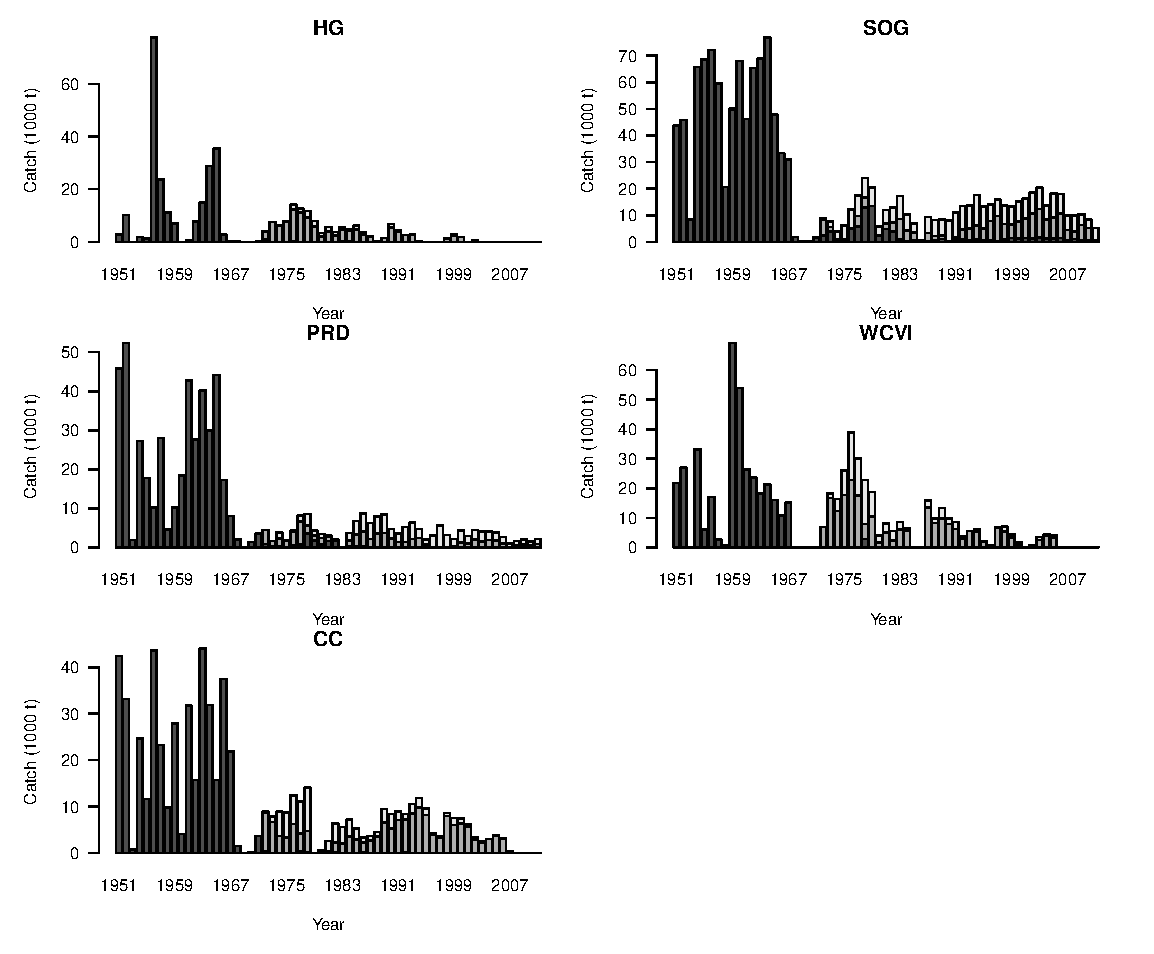
\includegraphics[width=\textwidth]{../Figs/iscam_fig_CatchMajorAreas.pdf}\\
	\caption{Historical catch of herring in the five major stock areas between 1951 and 2011 for the winter purse seine fishery (dark bars), seine-roe fishery (grey bars), and gillnet fishery (light grey bars). Units of catch are in thousands of metric tons.}\label{FigCatch}
\end{figure}
	
	\subsubsection{Relative abundance data}
Herring spawn surveys have been conducted throughout the B.C. coast beginning in the 1930s. Prior to 1988, spawn surveys were conducted from the surface either by walking the beach at low tide or using a drag from a skiff to estimate the shoreline length and width of spawn. Egg layers were sampled visually and are used to calculate egg densities following the methods of \cite{schweigert2001stock}. Beginning in 1988, herring spawn surveys using SCUBA methods were introduced and were implemented coastwide within a couple of years initially being conducted by DFO staff and eventually through contract divers hired through the test fishing program. Prior to the 2006 Larocque ruling, the test fishing program was funded through an allocation of fish by industry. In years since the 2006 Larocque ruling, the availability of resources to conduct dive surveys in all areas has been reduced. For 2011, dive surveys were conducted in all major and minor assessment regions, with the exception of Area 2W where snorkelling and surface survey methods were also used. As in earlier years, a few minor spawning beds outside the main assessment areas were surveyed by SCUBA or surface methods where resources permitted.


The locations of the spawning beds for the five major and two minor stock areas are shown in Figure \ref{figSpawnMaps}.  Egg density estimates are used to calculate a fishery-independent index of herring spawning biomass, referred to as the spawn survey index hereafter \citep{schweigert2001stock}.

\begin{figure}[!tbp]
	% Requires \usepackage{graphicx}
	\centering
	\includegraphics[scale=0.35]{../Figs/PBSfigs/2011_spawn_HG_2E_July13.pdf}
	\includegraphics[scale=0.35]{../Figs/PBSfigs/2011_spawn_HG_2W_July13.pdf}\\
	\includegraphics[scale=0.35]{../Figs/PBSfigs/2011_spawn_PRD_July13.pdf}
	\caption{Preliminary Spawning activity for Haida Gwaii (top panels) and Prince Rupert District (bottom) in 2011.}
\end{figure}
\begin{figure}[!tbp]
	% Requires \usepackage{graphicx}
	\ContinuedFloat
	\centering
	\includegraphics[scale=0.35]{../Figs/PBSfigs/2011_spawn_CCJuly13.pdf}
	%\includegraphics[scale=0.5]{../Figs/PBSfigs/2011-SOG-Prelim-WG.pdf}
	\includegraphics[scale=0.35]{../Figs/PBSfigs/2011_spawn_SOG_July13.pdf}\\
	\includegraphics[scale=0.35]{../Figs/PBSfigs/2011_spawn_WCVI_August16.pdf}
	\caption{Preliminary Spawning activity for Central Coast (top left panel), Strait of Georgia (top right) in 2011 and west coast Vancouver Island (bottom).}\label{figSpawnMaps}
\end{figure}
% \begin{figure}[!tbp]
% 	% Requires \usepackage{graphicx}
% 	\ContinuedFloat
% 	\centering
% 	%\includegraphics[scale=0.5]{../Figs/PBSfigs/2011-WCVI-Prelim-WG.pdf}\\
% 	\includegraphics[scale=0.5]{../Figs/PBSfigs/2011_spawn_WCVI_August16.pdf}\\
% 	\caption{Preliminary Spawning activity in 2011 for the West Coast of Vancouver Island (includes minor stock area 27).}\label{figSpawnMaps}
% \end{figure}

	The spawn survey is conducted after the fisheries in the area have been completed; therefore, it is assumed that all the mortality for the year has occurred just prior to commencing the spawning survey. The fisheries independent survey estimates egg density and total spawn area, and from this information the total female spawning biomass can be estimated assuming the 200 eggs per gram of female  or 100 eggs per gram of mature  individuals \citep{hay1985reproductive,hardwick1973biomass}. The assumed selectivity for the spawn survey is fixed to the maturity schedule for herring.  	
	
\begin{figure}[!tbp]
	% Requires \usepackage{graphicx}
	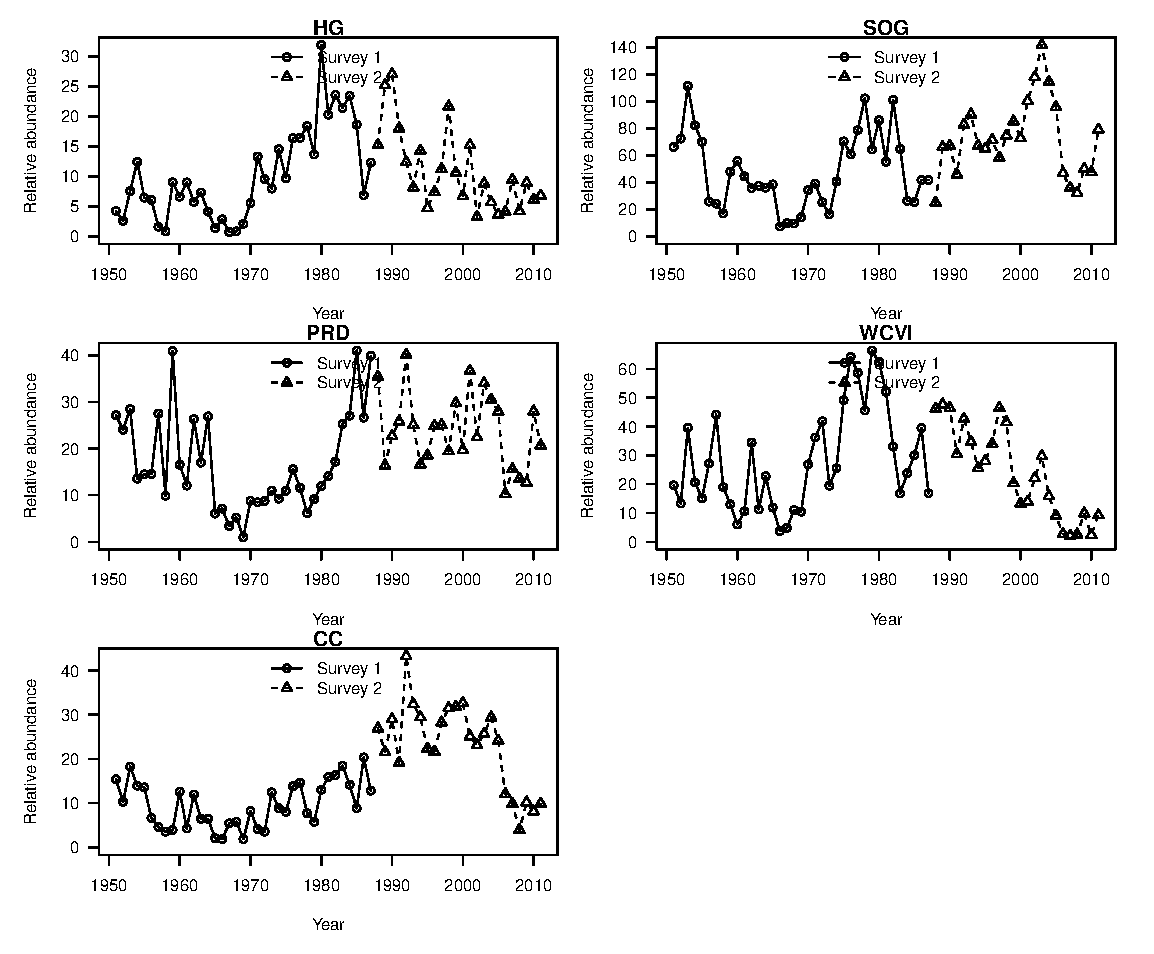
\includegraphics[width=\textwidth]{../Figs/iscam_fig_SurveyMajorAreas.pdf}\\
	\caption{Spawn survey index for Strait of Georgia between 1951 and 2011. The units are actual estimates of spawning biomass (1000s tons), but only the trend information is used in the model fitting.}\label{FigSurvey}
\end{figure}
	
	\subsubsection{Biological samples}
	
	Biological samples are collected from both commercial catch and from the test fishery program.  Commencing  in 1975, test fishery charters supplemented biological samples in areas with poor sampling that was not representative of the stock in that area (i.e., fishing solely on spawning aggregations), or in closed areas. Prior to 2006, test fishing charters were funded through an allocation of fish to the test program; the program is now fully funded by DFO.  Through a contract with DFO, the Herring Conservation and Research Society (HCRS) sub-contracts a number of vessels to collect biological samples.  Industry also conducts pre-season test sets for roe-quality testing in open areas and supplementary biological samples are provided as part of this program.  The following data are collected for all biological samples: fish length, weight, sex, and maturity.  Subsequently these sources of data are combined and information on weight-at-age and proportion-at-age become input data for the stock assessment model.
	
	During the 2010/2011 season a total of 248 biological samples were collected, of which 151 were collected from the test fishery, 57 were collected from the roe fishery, 16 from the food \& bait fishery, 4 from Spawn on Kelp (SOK) operations, and 16 from the summer trawl research survey (Table \ref{table:PartII:bioSamples}).  Note that the definition of a sample is roughly 100 individual fish.  A summary of biological samples collected from commercial and pre-fishery charters from 2002/03--2010/11 is presented in Table \ref{table:PartII:sampleSizes}).

\begin{table}
	\caption{Summary of biological samples collected and processed from all sources from the 2010/11 herring season.}
	\label{table:PartII:bioSamples}
	\begin{center}
		\begin{tabular}{cccccc}
		\hline
		& \multicolumn{3}{c}{Commercial samples} &  \\
		Stock & Roe fishery & SOK fishery & F\&B & Test fishery & Research\\
		\hline
		HG (QCI 2E) &  &  &  & 13\\
		PRD & 29 & 1 &  & 24\\
		CC &  &  &  & 30\\
		SOG & 18 &  & 20 & 60\\
		WCVI &  &  &  & 14 & 16\\
		Area 2W &  &  &  & 10\\
		Area 27 &  & 3\\
		Other Areas\\
		\hline
		Total & 57 & 4 & 16 & 151 & 16\\
		\hline
		\end{tabular}
	\end{center}
\end{table}

\begin{table}
	\caption{Summary of biological samples collected and processed from commercial catch and test fishery charters from 2002/03-2010/11.}
	\label{table:PartII:sampleSizes}
	\begin{center}
\begin{tabular}{cccc}
\hline
Fishing season & Commercial fishery samples & Charter and research samples & Total\\
\hline
2002/03 & 120 & 287 & 407\\
2003/04 & 79 & 222 & 301\\
2004/052 & 83 & 191 & 274\\
2005/06 & 46 & 164 & 210\\
2006/07 & 114 & 85 & 199\\
2007/08 & 116 & 103 & 219\\
2008/09 & 87 & 136 & 223\\
2009/10 & 78 & 135 & 213\\
2010/11 & 81 & 167 & 248\\
\hline
\end{tabular}
	
	\end{center}
\end{table}
	
	
	
	%%Insert Summary of biological samples from the 2010/2011 season here:
	
	%%Insert Summary of biological samples collected and processeed from commercial catch etc. here (Table 2 from Cleary 2011).
	
	\subsubsection{Age composition data}
	
	Ageing data, through the reading of fish scales, are collected from the biological samples taken from the commercial fisheries and test fishery charters. Age composition data is used to determine proportions-at-age and is an essential source of input data to the herring stock assessment model.
	
	Catch-at-age data from the winter seine fishery (top panels of Figures \ref{FigAgeCompsHG}-\ref{FigAgeCompsWCVI}) tend to consist of younger fish in comparison to the age composition data from the seine-roe and gillnet fleets post 1970. The shaded polygons in Figures \ref{FigAgeCompsHG}-\ref{FigAgeCompsWCVI} approximates the 95\% distribution of ages in the catch.  Roughly 90\% of the fish landed in the winter seine fishery were younger than age-7, and younger than age-6 in recent years.  In both the winter seine and seine-roe fishery age-2 fish are frequently landed; whereas, age-2 fish are rarely landed in the gillnet fishery, and fish do not appear to fully recruit to the gear until at least 4-5 years of age.  The mean age of the catch appears to be increasing between 2008 and 2010 in both the gillnet and winter seine fishery, and there is no obvious trend in the seine roe fishery.  There is however a declining trend in the older ages caught in the seine-roe fishery since 2006 (erosion of age-structure).

\begin{sidewaysfigure}[!tbp]
	% Requires \usepackage{graphicx}
	\centering
	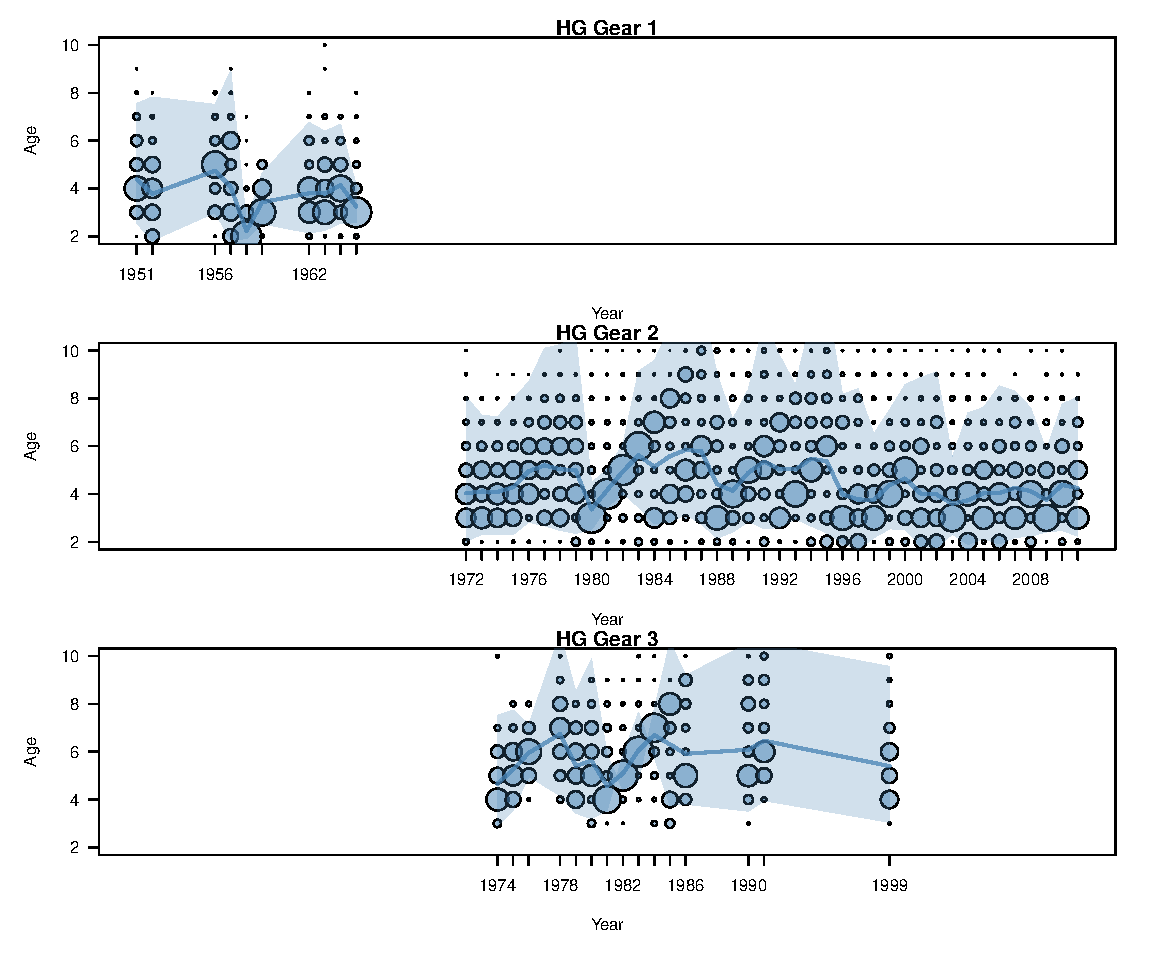
\includegraphics[width=0.85\textwidth]{../Figs/iscam_fig_AgeCompsHG.pdf}\\
	\caption{Bubble plots showing the proportions-at-age versus time for the winter purse seine fishery (top), seine roe fishery (middle) and the gillnet fishery (bottom) in Haida Gwaii.  The area of the circle is proportional to cohort abundance, each column sums to 1, zeros are not shown, and age 10 is a plus group. Also shown is the mean age of the catch (line) and the approximate 95\% distribution of ages (shaded polygon) for each year.}\label{FigAgeCompsHG}
\end{sidewaysfigure}

\begin{sidewaysfigure}[!tbp]
	% Requires \usepackage{graphicx}
	\centering
	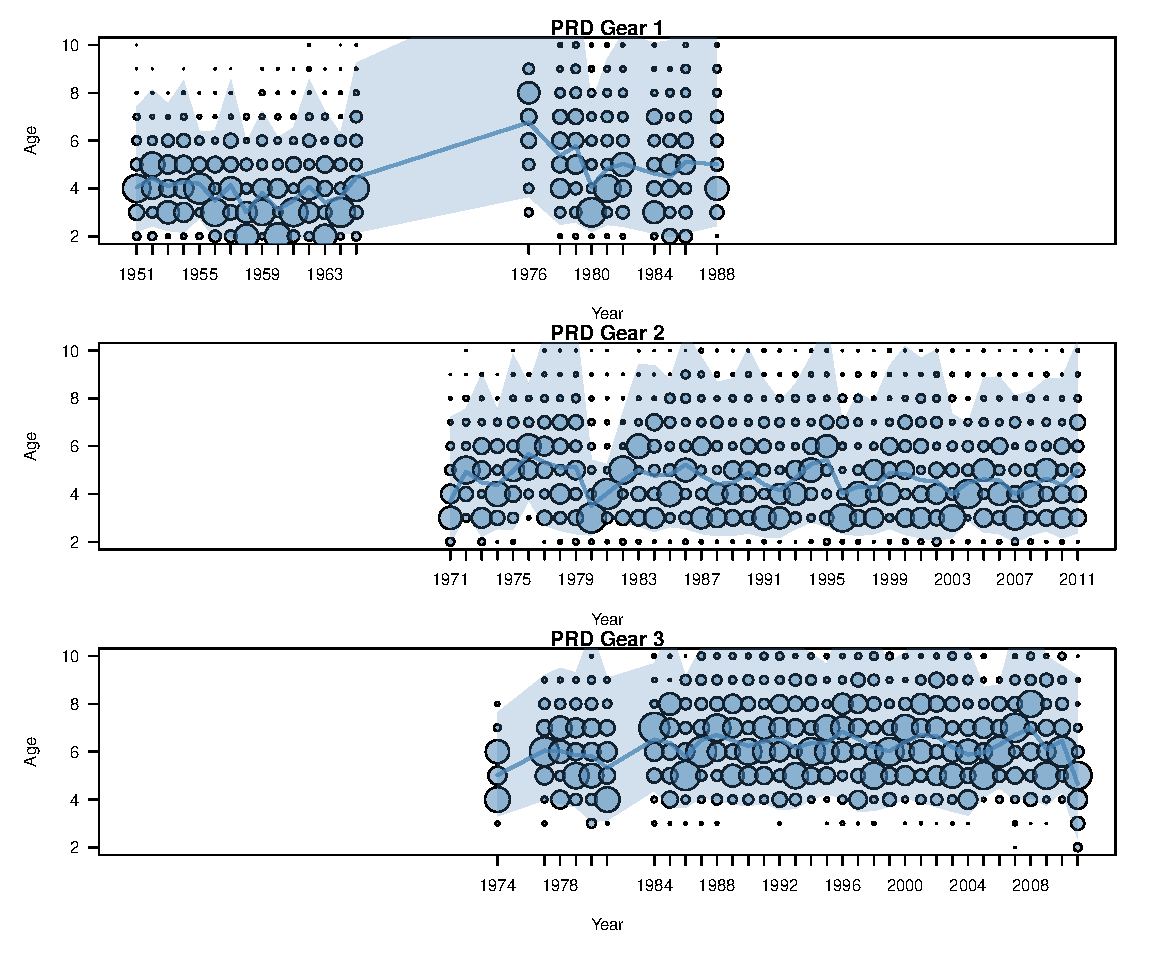
\includegraphics[width=0.85\textwidth]{../Figs/iscam_fig_AgeCompsPRD.pdf}\\
	\caption{Bubble plots showing the proportions-at-age versus time for the winter purse seine fishery (top), seine roe fishery (middle) and the gillnet fishery (bottom) in Prince Rupert District.  The area of the circle is proportional to cohort abundance, each column sums to 1, zeros are not shown, and age 10 is a plus group. Also shown is the mean age of the catch (line) and the approximate 95\% distribution of ages (shaded polygon) for each year.}\label{FigAgeCompsPRD}
\end{sidewaysfigure}

\begin{sidewaysfigure}[!tbp]
	% Requires \usepackage{graphicx}
	\centering
	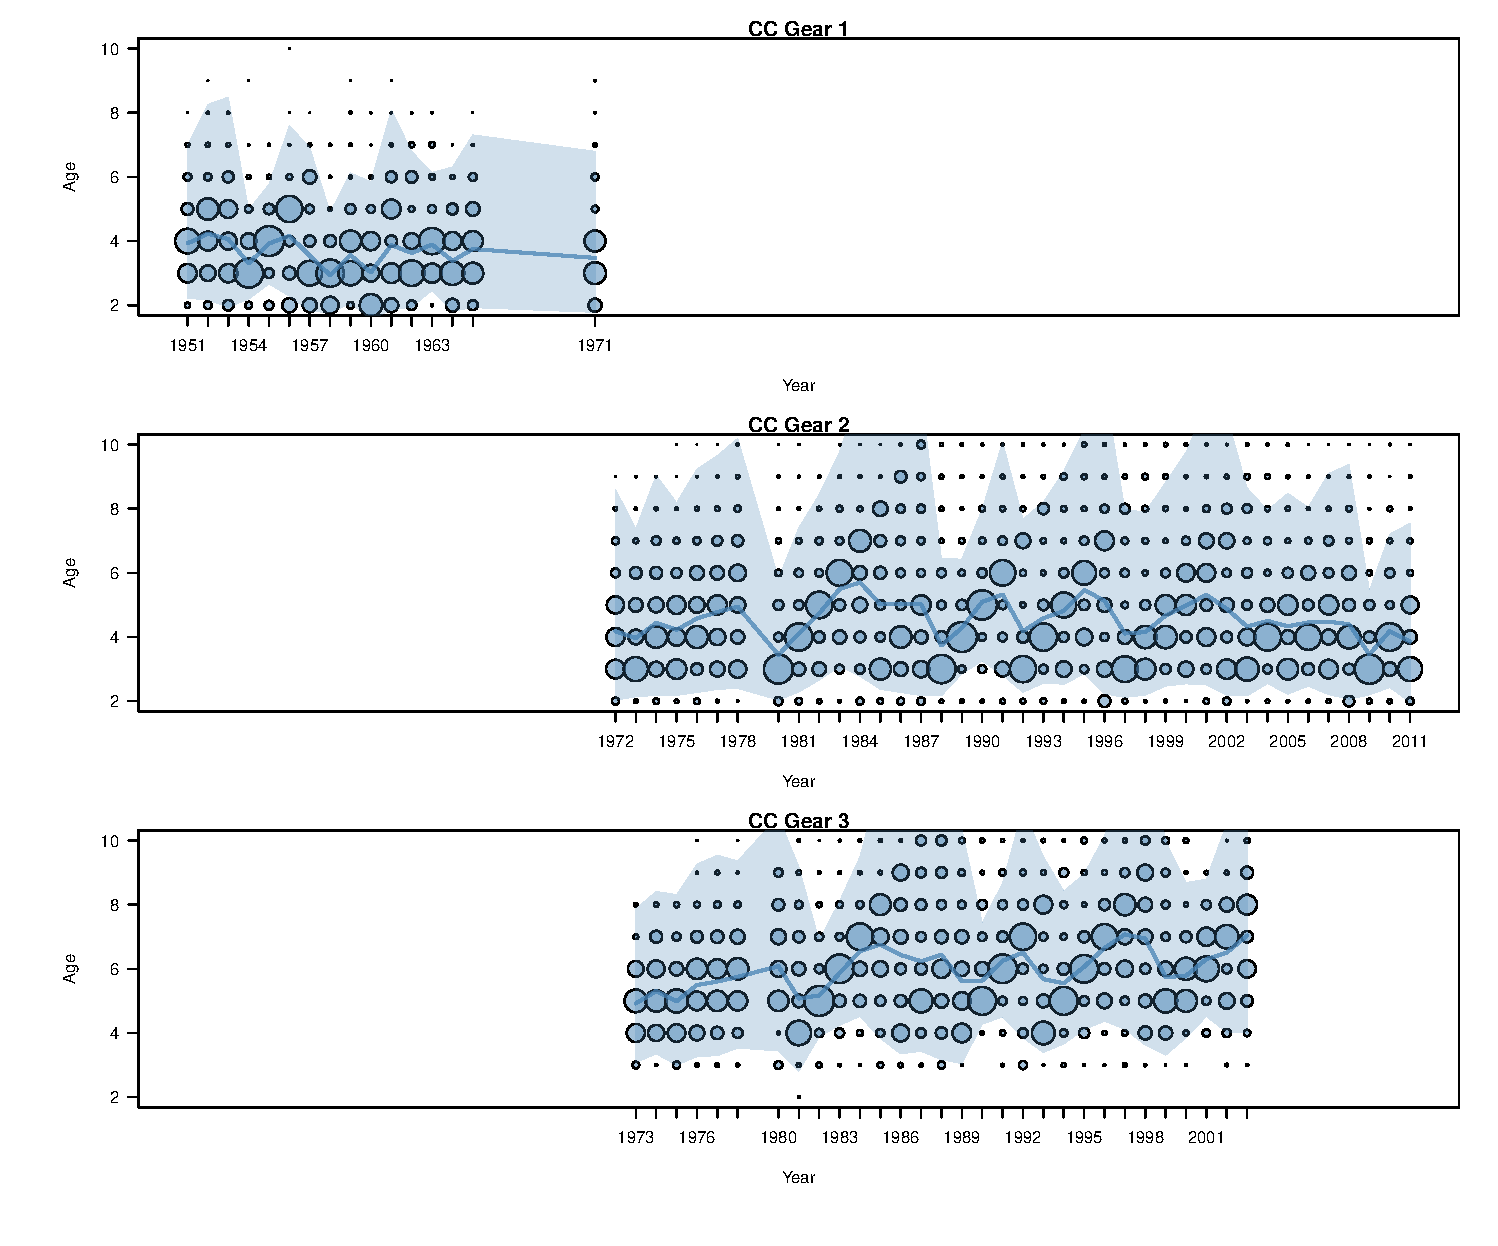
\includegraphics[width=0.85\textwidth]{../Figs/iscam_fig_AgeCompsCC.pdf}\\
	\caption{Bubble plots showing the proportions-at-age versus time for the winter purse seine fishery (top), seine roe fishery (middle) and the gillnet fishery (bottom) in the Central Coast region.  The area of the circle is proportional to cohort abundance, each column sums to 1, zeros are not shown, and age 10 is a plus group. Also shown is the mean age of the catch (line) and the approximate 95\% distribution of ages (shaded polygon) for each year.}\label{FigAgeCompsCC}
\end{sidewaysfigure}

\begin{sidewaysfigure}[!tbp]
	% Requires \usepackage{graphicx}
	\centering
	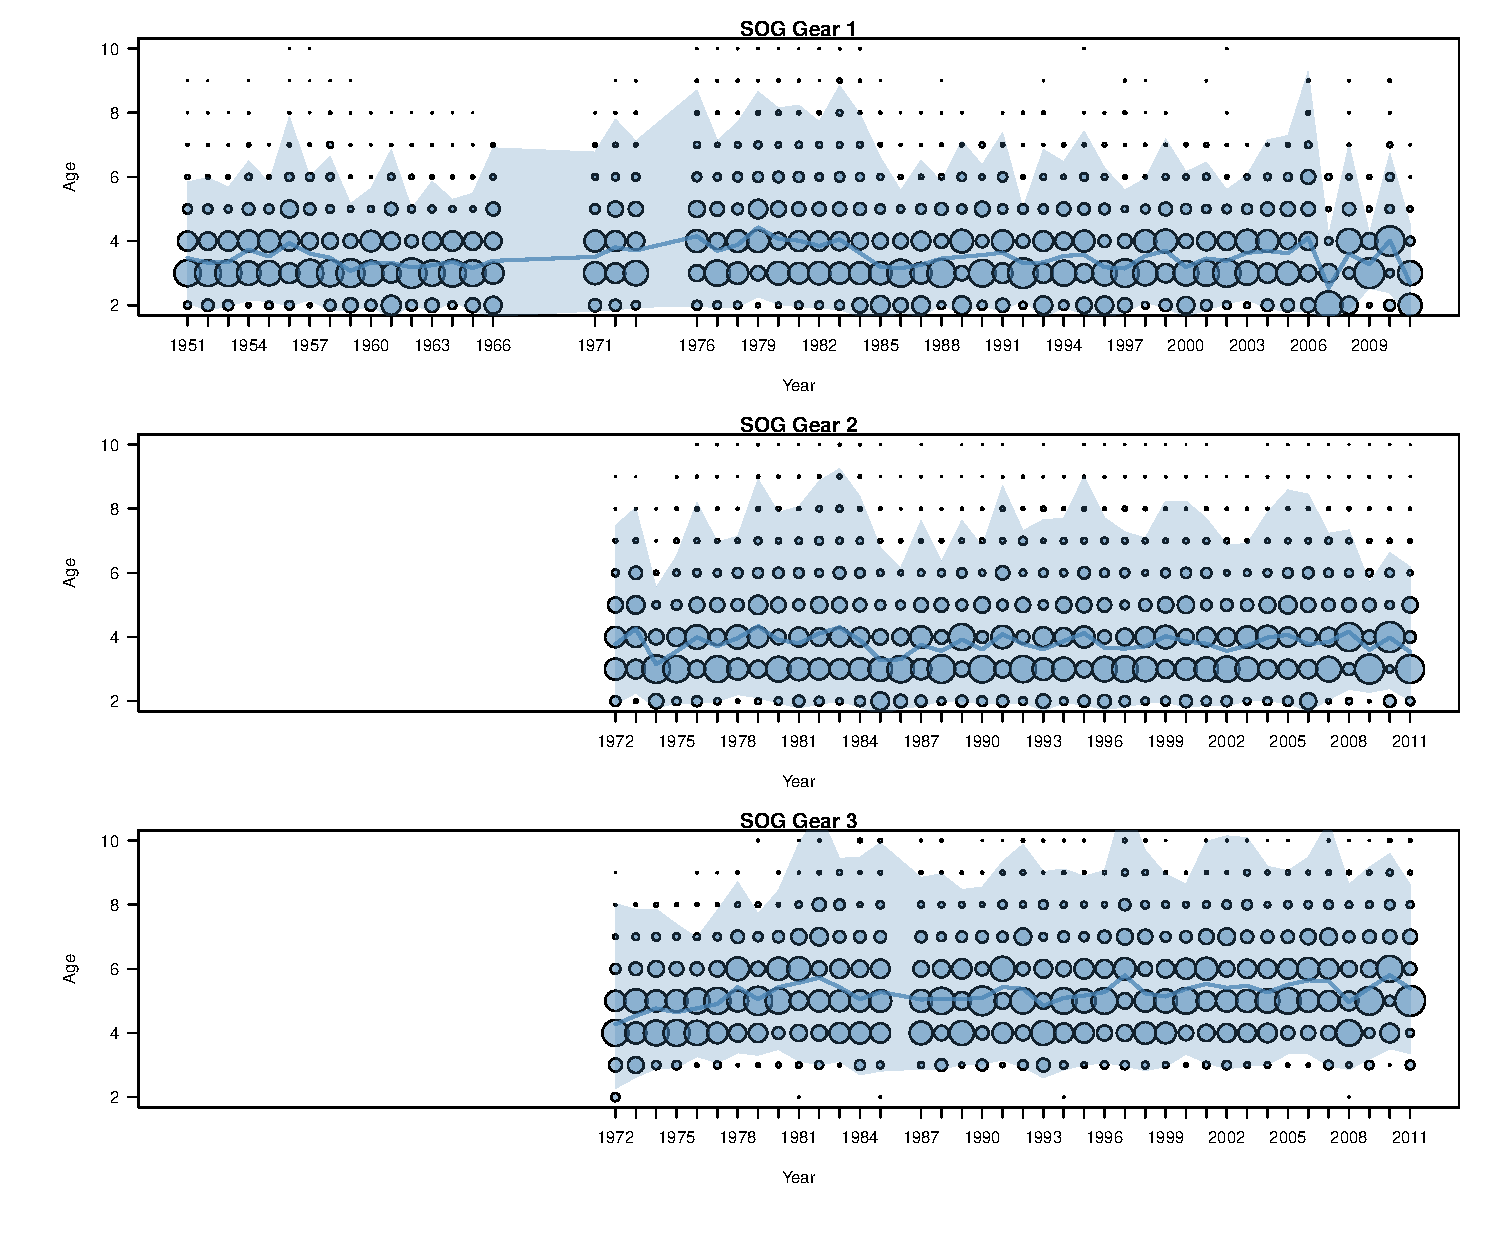
\includegraphics[width=0.85\textwidth]{../Figs/iscam_fig_AgeCompsSOG.pdf}\\
	\caption{Bubble plots showing the proportions-at-age versus time for the winter purse seine fishery (top), seine roe fishery (middle) and the gillnet fishery (bottom) in the Strait of Georgia.  The area of the circle is proportional to cohort abundance, each column sums to 1, zeros are not shown, and age 10 is a plus group. Also shown is the mean age of the catch (line) and the approximate 95\% distribution of ages (shaded polygon) for each year.}\label{FigAgeCompsSOG}
\end{sidewaysfigure}

\begin{sidewaysfigure}[!tbp]
	% Requires \usepackage{graphicx}
	\centering
	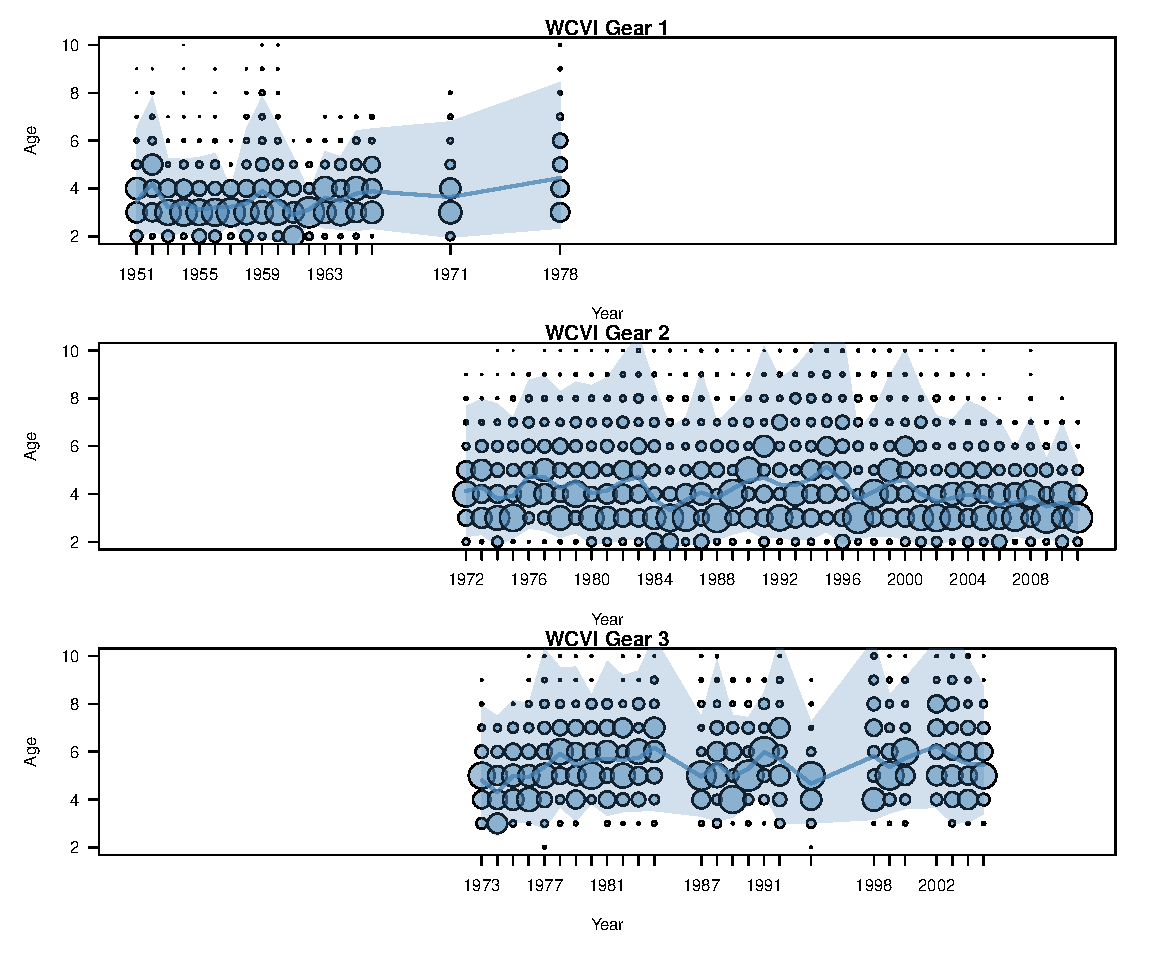
\includegraphics[width=0.85\textwidth]{../Figs/iscam_fig_AgeCompsWCVI.pdf}\\
	\caption{Bubble plots showing the proportions-at-age versus time for the winter purse seine fishery (top), seine roe fishery (middle) and the gillnet fishery (bottom) in the West Coast Vancouver Island region.  The area of the circle is proportional to cohort abundance, each column sums to 1, zeros are not shown, and age 10 is a plus group. Also shown is the mean age of the catch (line) and the approximate 95\% distribution of ages (shaded polygon) for each year.}\label{FigAgeCompsWCVI}
\end{sidewaysfigure}





	\subsubsection{Mean weight-at-age data}

	From the mid-1970s until the present, there has been a measurable decline in weight-at-age for all ages in all major stock areas (Figure \ref{FigMeanWt}). Samples collected during the 2009/10 fishing year indicate weights-at-age that are among the lowest on record. This declining weight-at-age may be attributed to any number of factors, including: fishing effects (i.e., gear selectivity), environmental effects (changes in ocean productivity), or it may even be attributed to changes in sampling protocols (shorter time frame over which samples are collected). Declining weight-at-age has been observed in all five of the major stocks, and despite area closures over the last 10-years, has continued to occur in the QCI and WCVI stocks. Although the direct cause of this decline is still to be investigated, this trend has been observed in B.C. and U.S. waters, from California to Alaska \citep{schweigert2002herring}, and merits further research.	The observed mean weight-at-age data appear to have a few  errors that need to be investigated as well; for example, see the apparently small age-10 fish in 2001 in Figure \ref{FigMeanWt}.

\begin{figure}[!tbp]
	% Requires \usepackage{graphicx}
	\centering
	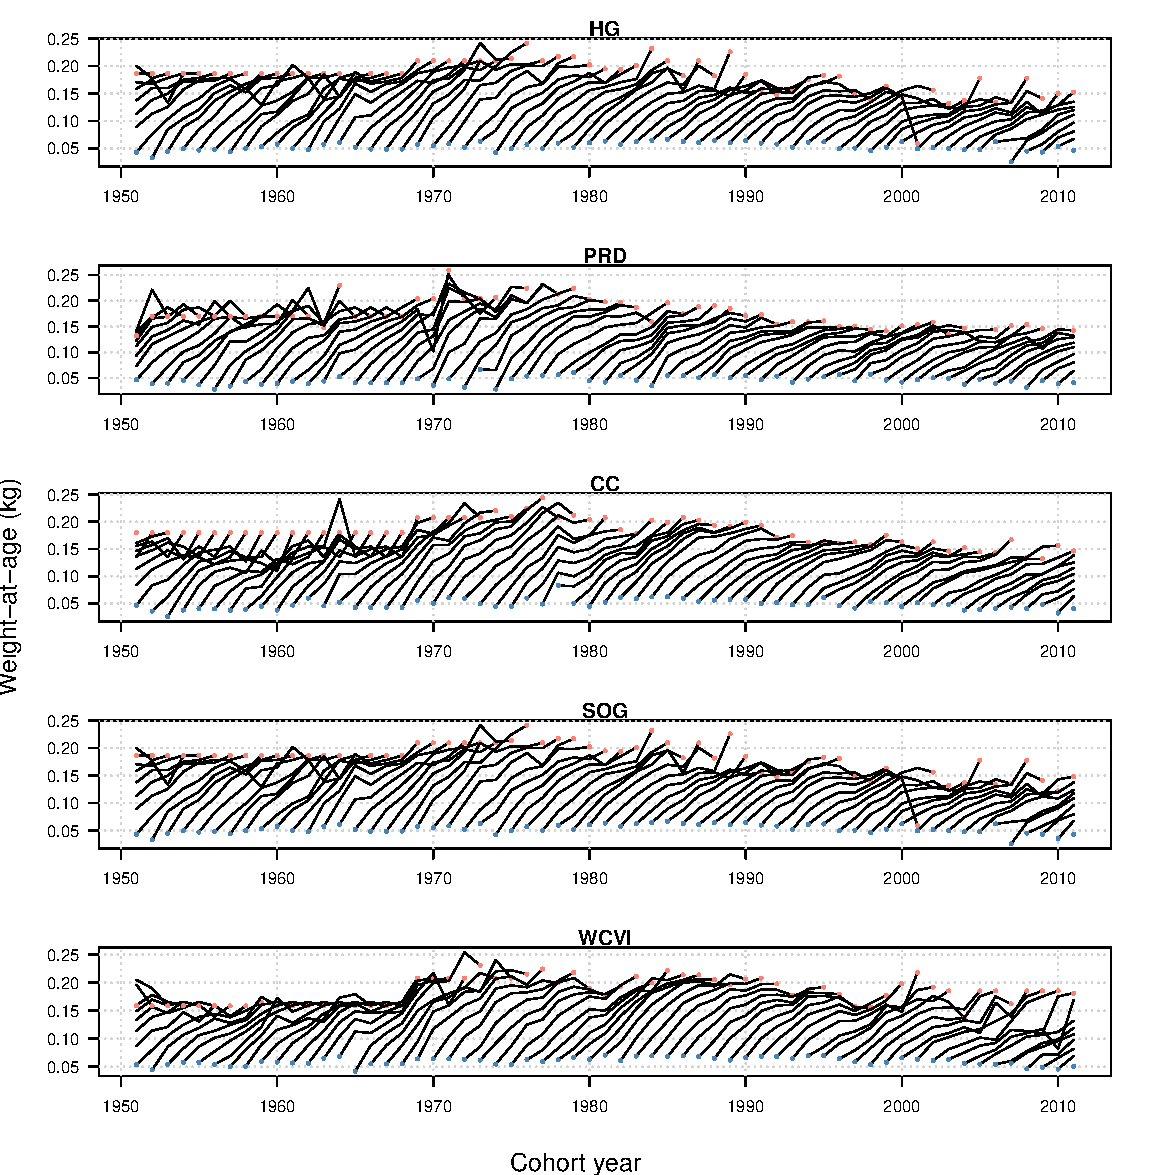
\includegraphics[width=\textwidth]{../Figs/iscam_fig_MeanWt.pdf}\\
	\caption{Empirical mean weight-at-age data by cohort from 1951 to 2011 for ages 2 to 10 in the five major Stock Assessment Regions.}\label{FigMeanWt}
\end{figure}
	

%%%%%%%%%%%%%%%%%%%%%%%%%%%%%%%%%%%%%%%%%%%%%%%%%%%%%%%%%%%%%%%%%%%%%
%%%%%%%%%%%%%%%%%%%%%%%%%%%%%%%%%%%%%%%%%%%%%%%%%%%%%%%%%%%%%%%%%%%%%
%%%%%%%%%%%%%%%%%%%%%%%%%%%%%%%%%%%%%%%%%%%%%%%%%%%%%%%%%%%%%%%%%%%%%	
	\subsection{Analytical methods}

	For the 2011 BC herring assessment, \iscam was used to conduct the stock assessment for each of the five major Stock Assessment Regions (SAR) and two minor assessment areas (Area 2W and Area 27).  The technical details of this model can be found in Appendix \ref{appiSCAM}.
		
	\subsection{Retrospective analysis}
	A retrospective analysis was conducted for each of the major and minor SARs.  The retrospective analysis successively removes the last 10-years of data and examines changes in estimates of terminal spawning biomass.  The results are then plotted on a single panel to compare how estimates of spawning biomass change as successive years of data are omitted from the analysis.
	
	\subsection{Abundance and recruitment forecasts}
	The abundance forecast for the upcoming fishing season, also referred to as pre-fishery biomass, is defined as the predicted biomass of age-4 fish and older plus the number of age-3 fish recruiting in year $T+1$.  The abundance estimates are based on the median values from the sampled posterior distribution.  Age-3 recruits are based on poor, average, and good recruitment scenarios; see next paragraph for definitions of poor, average and good.
	
	The recruitment forecasts are based on the surviving number of age-3 fish at the start of the fishing season times the average weight-at-age 3 in the last 5 years. The definitions of poor, average, and good recruitment are as follows: \textbf{Poor} is the average recruitment from the 0-33 percentile, \textbf{Average} is the average recruitment from the 33-66 percentile, and \textbf{Good} is the average recruitment from the 66-100 percentile.  Note that all cohorts from 1951 to 2011  were included in the calculation of recruitment quantiles.
	
	\subsection{Catch advice}
Catch advice is based on the application of the harvest control rule (HCR). The herring HCR has three components:
\begin{enumerate}
\item Reference points (LRP, USR, and cuttoffs)
\item Harvest rate
\item Decision rules
\end{enumerate}

For each of the five major stocks, the limit reference point (LRP) is the cuttoff value, which is defined here as 0.25\bo\, and the	Upper Stock Reference (USR) is defined as the 1.05*LRP (0.25\bo\ + 0.2*0.25\bo = LRP + 0.05LRP). \textbf{For clarification, references to \bo\ throughout this document refer to the mature spawning stock biomass.} The default harvest rate if the stock is at or above USR is 0.2, and declines linearly to 0 when the stock is at or below the LRP (a default harvest rate of 0.1 is used for the minor stock areas).  The decision rule for the major stock areas operates as follows:

\begin{itemize}
	\item If the forecast run is less than the LRP (cuttoff) then the area is closed to all commercial harvest  (i.e., stock is deemed to be in the critical zone).
	
	\item If the forecast run is greater than the LRP and less than the USR (i.e., cautious zone), then total allowable catch is based on a reduced harvest rate that would deplete the stock to the LRP level.
	
	\item If the forecast run is greater than USR, then the total allowable catch is set at 20\% of the forecast run.
\end{itemize}



	

%    %!TEX root=../Selex.tex
% Statisitcal fit

% Retrospective performance.

% Estimated reference points.

\section*{Results} % (fold)
\label{sec:results}

\subsection*{Statisical fit} % (fold)
\label{sub:statisical_fit}

Statisitics summarizing how well each model fits a single realization of simulated data are based on the overall objective function value, Deviance Information Criterion (DIC) and the Root Mean Square Error (RMSE) between observed and predicted quantities (Table \ref{tab:statisticalPeformance}). Under conditions in which the true selectivity is fixed (scenmario 1), similar fits to the relative survey abundance index and age-composition data (see Survey RMSE and Survey age RMSE in Table \ref{tab:statisticalPeformance}) were obtained  irrespective of the form of the assumed selectivity curve for the commercial fishery.  However, fits to the commercial age-composition data markedly improved under the time-varying age-based selectivity model (c).  Allowing for additional structure in the selectivity coefficients over time resulted in decreases in the RMSE from 0.48, 0.41 and 0.33 for models (a), (b), and (c), respectively for the commercial age-composition information (Table \ref{tab:statisticalPeformance}).  The worst fit to the commercial age-composition was obtained for the bicubic spline model (d).

We do not recommend basing model selection solely on statistical criterion, such as DIC, but for statistical comparison we provide DIC and $\Delta$DIC values to give a sense of the relative differences between the various assessment models for each simulation case.  In the cases examined here (Table \ref{tab:statisticalPeformance}), DIC always favors the most structurally complex model (c) with the largest number of estimated selectivity parameters. The large improvement in fit for model (c) is always due to explaining more residual variation in the age-composition data. All other models appear to fit the survey index and age-composition equally, regardless if the data were generated from fixed selectivities or complex time-varying selectivities.  This is not an unexpected result, as the observation models for the survey age composition data are structurally consistent with the simulation model.  What is significant is that the use of the conditional maximum likelihood estimate of the variance to weight the commercial age-composition data is down-weighted when the incorrect selectivity model is specified for the commercial selectivities. However, it should be noted that this down-weighting incorrectly assigns process error to observation error due to mis-specification of selectivity.




\begin{table*}[!tbh]
	\caption{Statistical performance based on the objective function value, effective number of estimated parameters, DIC, $\Delta$DIC, Root Mean Square Error (RMSE) in recruitment deviations, survey abundance residuals, and the age-composition residuals for models fit to fixed, discrete time blocks and continous changes in commercial selectivity.}
	\label{tab:statisticalPeformance}
	\begin{center}
		\begin{tabular}{l|cccc}
		\hline

		\hline
		\textbf{} & \textbf{Fixed (a)} & \textbf{Discrete (b)} & \textbf{Continuous (c)} & \textbf{Bicubic spline (d)} \\
		\hline

		
	    \multicolumn{5}{l}{\textbf{\underline{True selectivity is fixed}}}\\
		Objective function            &  -836.41 &  -918.16 & -1208.16 &  -939.17 \\
		Eff. No. parameters             &    96 &   116 &   334 &   173 \\
		DIC              & -1479.77 & -1601.51 & -1739.09 & -1528.01 \\
		$\Delta$DIC         &   259.32 &   137.58 &     0.00 &   211.08 \\
		Recruitment RMSE &     1.04 &     1.04 &     1.06 &     1.04 \\
		Survey RMSE      &     0.25 &     0.25 &     0.26 &     0.26 \\
		Commercial RMSE         &     0.47 &     0.40 &     0.32 &     0.49 \\
		Survey age RMSE         &     0.24 &     0.25 &     0.25 &     0.24 \\
		%Total.RMSE       &     2.03 &     1.96 &     1.90 &     2.06 \\
		
		\hline
		\multicolumn{5}{l}{\textbf{\underline{True selectivity has 3 time blocks}}}\\
		Objective function            &  -775.49 & -1051.57 & -1335.82 & -1028.80 \\
		Eff. No. parameters             &    96 &   116 &   337 &   173 \\
		DIC              & -1356.24 & -1868.57 & -1990.44 & -1707.88 \\
		$\Delta$DIC         &   634.20 &   121.87 &     0.00 &   282.56 \\
		Recruitment RMSE &     1.04 &     1.04 &     1.05 &     1.05 \\
		Survey RMSE      &     0.26 &     0.26 &     0.26 &     0.26 \\
		Commercial RMSE         &     0.52 &     0.35 &     0.29 &     0.45 \\
		Survey age RMSE         &     0.25 &     0.29 &     0.25 &     0.24 \\
		%Total.RMSE       &     2.10 &     1.92 &     1.86 &     2.02 \\

		\hline
		\multicolumn{5}{l}{\textbf{\underline{True selectivity changes annually}}}\\
		Objective function            &  -717.56 &  -788.52 & -1029.41 &  -785.91 \\
		Eff. No. parameters             &    96 &   116 &   333 &   173 \\
		DIC              & -1241.22 & -1342.26 & -1382.43 & -1222.14 \\
		$\Delta$DIC         &   141.21 &    40.17 &     0.00 &   160.29 \\
		Recruitment RMSE &     1.06 &     1.09 &     1.12 &     1.05 \\
		Survey RMSE      &     0.26 &     0.26 &     0.27 &     0.26 \\
		Commercial RMSE         &     0.52 &     0.44 &     0.35 &     0.56 \\
		Survey age RMSE         &     0.27 &     0.29 &     0.30 &     0.27 \\
		%Total.RMSE       &     2.14 &     2.10 &     2.07 &     2.17 \\



		% Objective function  & -1452.78 &  -1461.06 &  -1695.12 &  -1538.09 \\
		% Eff. No. parameters &    96    &    110    &    344    &    175    \\
		% DIC                 & -2712.84 &  -2701.20 &  -2696.89 &  -2723.12 \\
		% $\Delta$DIC         &    10.28  &    21.92 &     26.23 &      0.00 \\
		% Recruitment RMSE    &     1.03 &      1.03 &      1.03 &      1.03 \\
		% Survey RMSE         &     0.25 &      0.26 &      0.25 &      0.25 \\
		% Commercial RMSE     &     0.28 &      0.28 &      0.20 &      0.26 \\
		% Survey age RMSE     &     0.26 &      0.26 &      0.27 &      0.26 \\

		
		% \hline
		% Objective function  & -1340.49 &  -1428.81 &  -1689.57 &  -1516.78 \\
		% Eff. No. parameters &    96    &    109    &    345    &    175    \\
		% DIC                 & -2487.96 &  -2638.03 &  -2683.48 &  -2680.78 \\
		% $\Delta$DIC         &   195.52 &     45.45 &      0.00 &      2.70 \\
		% Recruitment RMSE    &     1.04 &      1.04 &      1.03 &      1.03 \\
		% Survey RMSE         &     0.25 &      0.26 &      0.25 &      0.25 \\
		% Commercial RMSE     &     0.32 &      0.29 &      0.20 &      0.26 \\
		% Survey age RMSE     &     0.26 &      0.26 &      0.27 &      0.26 \\

		
		% \hline
		% Objective function  & -1293.30 &  -1304.14 &  -1543.59 &  -1376.39 \\
		% Eff. No. parameters &    95    &    109    &    344    &    177    \\
		% DIC                 & -2394.61 &  -2387.88 &  -2393.28 &  -2396.33 \\
		% $\Delta$DIC         &     1.72 &      8.45 &      3.05 &      0.00 \\
		% Recruitment RMSE    &     1.13 &      1.13 &      1.12 &      1.12 \\
		% Survey RMSE         &     0.26 &      0.27 &      0.27 &      0.27 \\
		% Commercial RMSE     &     0.30 &      0.30 &      0.21 &      0.28 \\
		% Survey age RMSE     &     0.33 &      0.34 &      0.33 &      0.32 \\

		\hline

		\hline
		\end{tabular}
	\end{center}
\end{table*}
The effective number of estimated parameters is based on the difference between the expectation of the deviance and the deviance based on the expectation of the parameter values.  The larger the effective number of parameters is a measure of how well the model fits the data.  In all cases the effective number of parameters was equal to or greater than the number of parameters estimated in the model.  In the case of model (c) the effective number of parameters ($\approx$335) is much greater than the 319 that were actually estimated in the ADMB code.  However, it should also be noted that the variance parameters for age-composition residuals and the scaling parameter $q$ \citep[see][]{walters1994calculation} are based on the conditional maximum likelihood estimates, rather than explicitly estimating them inside the model code.  This parameterization implies an additional 67 parameters and hence the effective number of parameters is much less than the 386 parameters in model (c).  Again, we caution the use of DIC for model selection in cases where data are weighted via conditional maximum likelihood estimate of the variance.


% For the cases where the true selectivity is based on a fixed logistic function, the most appropriate model based on DIC is model (d) where a bicubic spline is used to model selectivity. The RMSE terms for model (d) are less than the true underlying values that were used to generate the data, which is of no surprice when additional flexibility in selectivity can accomodate some of the residual variance in age-composition in the form of minor changes in selectivity (Table \ref{tab:statisticalPeformance}).   This pattern of explaining the residual variation is virtually the same regardless of what the true underlying selectivity pattern is.

% In the case where the true selectivity changes discretely over three time blocks, assessment models with time-varying selectivity (c) and (d) appear to fit the data better that models that assumed fixed selectivity (a), or even the discrete changes in selectivity (see $\Delta$DIC values in Table \ref{tab:statisticalPeformance}).  For this particular case, it's better to allow for continous changes in selectivity than to 
% assume fixed values.

% In the case where the true selectivity changes annually, based on relative cohort abundance, the model results were a bit more surprising.  The expectation would be that assuming fixed selectivity would perform less well than allowing for time-varying selectivity.  Based on the $\Delta$DIC values obtained in Table \ref{tab:statisticalPeformance} there is very little differnce between models that allow for continous changes in selectivity (models c and d) and fixed selectivity (model a).  There was less weight for the model that allows for discrete-block changes in selectivity (model b).

% Similar results were also obtained in the case where true selectivity changes annually (as a function of the relative cohort abundance).  However, the difference between assuming block selectivity and fixed selectivity resulted in negligble differences in the $\Delta$AIC values.  Moreover, the RMSE for the age-composition data was greater than the true values used to generate the observation errors in age-sampling in models (a) and (b). For model (c), the RMSE was less than the true value for the commercial age-composition, and  in model (d) it was identical to the true value.   

% subsection statisical_fit (end)
\subsection*{Retrospective performance} % (fold)
\label{sub:retrospective_performance}

Two useful graphical tools for examining retrospective problems in stock assessment models are referred to here as spaghetti plots (Fig. \ref{fig:retrospectiveSSB}), and squid plots (Fig. \ref{fig:retrosquidbase}), respectively.  In the spaghetti plots, successive estimates of spawning stock biomass based on sequentially removing the terminal year of data for four previous years are overlayed on each panel.  In addition to the estimated spawning biomass in Fig. \ref{fig:retrospectiveSSB}, the true spawning biomass that was used to generate simulated data is also shown for reference.  In the squid plots, successive estimates of spawning biomass relative to the  spawning biomass in the terminal year of data are overlaid.  In Fig. \ref{fig:retrosquidbase}, the percent bias is shown as the relative difference between the true values; hence a 100\% bias implies that the stock size is over-estimated by a factor of 2.  


\begin{figure*}[!tbh]
	\begin{center}
		\includegraphics[angle=0,width=\textwidth]{./FIGS/fig:RetroSpectiveSSB.png}
	\end{center}
	\caption{One realization of retrospective estimates of spawning biomass for simulated Pacific hake populations where four years of data was sequentially removed from.  The true spawning biomass used to simulated the data is included for reference.}
	\label{fig:retrospectiveSSB}
\end{figure*}

Based on the maximum likelihood results from a single realization shown in Fig. \ref{fig:retrospectiveSSB}, there is a tendency for the model to systematically over-estimate the spawning stock biomass in the terminal years.  This trend is largely a function of the recent downward trend in abundance since the mid 2000s, and not a persistent feature of the stock assessment model.  In the case of the true selectivity being fixed over time, the least amount of retrospective bias occurred in the simple models (a) and (b), and the largest bias was observed for model (c).  Similar results were also obtained in the discrete changes in selectivity (row 2 of Fig. \ref{fig:retrosquidbase}) as well as the time-varying changes in selectivity.  Also of interest is the retrospective behavior in model (d) where the sequential removal of the terminal year data results in changing the knot positions in the bicubic spline (see early years on column (d) of Fig. \ref{fig:retrosquidbase}). Retrospective  estimates of spawning biomass earlier in the time series of model (d) are slightly more variable in comparison to models with fixed selectivities (a), (b), and even in the case where selectivity is allowed to vary annually (c).  However, these results are from a single realization, and should not be used to make general inferences in retrospective bias.  Median values from a series of Monte Carlo trials would be more appropriate for making general inferences.  These results from a single realization merely illustrate that despite additional structural flexibility associated with time-varying selectivity, large retrospective bias can still occur. 



% For the simulated data based on fixed selectivity, the qualitative pattern in retrospective bias was similar for all four alternative selectivity scenarios (Figure \ref{fig:retrospectiveSSB}, 1a, ..., 1d).   The worst performing models were the cases with continuous changes in selectivity over time (1c and 1d), with maximum estimates of retrospective bias relative to the terminal values approaching 25\% for the bicubic spline model (Figure \ref{fig:retrosquidbase}).  

% For cases based on simulated data with discrete time blocks in selectivity, the least amount of bias was observed in the case where the correct model was specified (Figure \ref{fig:retrosquidbase}, 2b).  Assuming fixed selectivity or continuous changes in selectivity resulted in significantly more retrospecitve bias.  Assuming fixed selectivity also resulted in further departures from the true spawning biomass in the initial years.

\begin{figure*}[!tbh]
	\begin{center}
		\includegraphics[angle=0,width=\textwidth]{./FIGS/fig:RetroSquidBase.png}
	\end{center}
	\caption{One realization of retrospective estimates of bias in spawning biomass relative to spawning biomass estimated with all available data.  These biases are based on the same spawning biomass trajectories in Figure \ref{fig:retrospectiveSSB}.}
	\label{fig:retrosquidbase}
\end{figure*}


% \begin{figure}[tb]
% 	\begin{center}
% 		\includegraphics[angle=90,width=0.85\textwidth]{../FIGS/fig:RetroSquid.png}
% 	\end{center}
% 	\caption{Retrospective estimates of bias in spawning biomass relative to the true spawning biomass used to simulated the data.  These biases are based on the same spawning biomass trajectories in Figure \ref{fig:retrospectiveSSB}.}
% 	\label{fig:retrosquid}
% \end{figure}

% In the cases where the true selectivity varies over time, the retrospective performance was least biased for the models that assume time-varying selectivity (Figure \ref{fig:retrosquidbase}, 3c and 3d).  Retrospective peformance is much worse if the selectivity is assumed to be constant, or change in a series of blocks, when the real underlying process is continuous change in selectivity (Figure \ref{fig:retrosquid}, 3a and 3b). 

% Monte Carlo retrospective results. Make general statement that less retrospective bias when assuming more structural complexity.  May be better to assume a penalized random walk in selectivity than to not.

Over a number of Monte Carlo trials (40 independent data sets) the patterns in retrospective bias over the alternative selectivity assumptions differ from the single realization shown in Fig. \ref{fig:retrospectiveSSB}.  To quantify retrospective bias, a series of summary statistics were used to measure the trade-off between precision and bias in the retrospective analyses (Table \ref{tab:RetroStatistics}).  The mean bias $\mu$ reflects the average difference between the terminal and retrospective year spawning biomass and is generally lowest for models that allow for time-varying selectivity (models (c) and (d) in Table \ref{tab:RetroStatistics}).  The absolute mean bias $|\mu|$ better characterizes the mean retrospective  variation.  For example, in model 3c (Table \ref{tab:RetroStatistics}) the mean bias $\mu$ is relatively small, but the mean absolute difference over four retrospective years is very large.  This is also reflected in the summary statistic $\Omega$ and the Mean Absolute Deviation (MAD).  Even though model 3c is the correct model for the simulations with continuous changes in selectivity, the results in Table \ref{tab:RetroStatistics} suggest that model 3d would be preferable due to less mean bias and a lower overall variance in the potential bias.  

\begin{table*}[!tbh]
	\caption{Retrospective bias statistics for each model run, where $\mu_1$ corresponds to the mean bias over four retrospective years, $\mu_2$ is the absolute mean, $\Omega$ is a combined measure of mean and absolute bias, and MAD is the Mean Absolute Deviation of $\mu_2$.  Lower MAD scores imply less variability in retrospective bias estimates.}
	\label{tab:RetroStatistics}
	\begin{center}
	\begin{footnotesize}
		
		\begin{tabular}{l|cccc|cccc|cccc}
		\hline

		\hline
		&\multicolumn{4}{c|}{\textbf{Fixed}} & \multicolumn{4}{c|}{\textbf{Discrete}} & \multicolumn{4}{c}{\textbf{Continous}} \\
		&\textbf{1a}  &\textbf{1b}  &\textbf{1c}  &\textbf{1d}  &\textbf{2a}   &\textbf{2b}  &\textbf{2c}  &\textbf{2d}  &\textbf{3a}  &\textbf{3b}  &\textbf{3c}  &\textbf{3d}\\
		\hline
		$\mu_1$     &-9.14& -8.26& -1.55& -1.77& -8.88& -12.57& -1.11& -3.11& -6.72& -5.90& -2.09& -0.83\\
		$\mu_2$ &14.19& 13.63& 13.46& 12.78& 12.94&  14.96& 12.12& 13.75& 14.06& 14.08& 17.99& 13.85\\
		$\Omega$  &19.13& 18.28& 17.49& 16.53& 17.58&  20.66& 15.73& 17.86& 18.62& 18.47& 22.97& 18.08\\
		MAD    & 4.77&  4.68&  6.42&  4.93&  5.32&   6.28&  5.11&  5.48&  4.73&  4.84& 10.51&  5.78\\

		\hline

		\hline
		\end{tabular}
	\end{footnotesize}
	\end{center}
\end{table*}

Similar results were also obtained for the simulations involving fixed selectivities and discrete time blocks with less overall mean bias, and lower MAD's, for models with continuous changes in selectivity over time (Table \ref{tab:RetroStatistics}).


% subsection retrospective_performance (end)


\subsection*{Estimated reference points} % (fold)
\label{sub:estimated_reference_points}


The impacts of model specification on the estimates of MSY-based reference points are summarized using a series of box-plots (Fig. \ref{fig:RefPointBias}) based on Monte Carlo trials.  In each box plot the $\ln$ ratios of the estimated versus true values are shown where the median bias is based on the solid bar.  In the case where the true model is based on fixed selectivity, estimated reference points are relatively unbiased ($\pm$ 10\%); however, the precision of the estimates decreases with increasing model complexity (Fig. \ref{fig:RefPointBias}).  There is a bit of a trend in the estimate of $F_{\rm{MSY}}$ that corresponds to an increase in overall stock productivity with assumed increases in model complexity.  This same increasing trend is also present, but less pronounced, in the estimates of MSY.  These trends indicate that the overall scale and productivity of the estimated population increases with increasing model complexity. 

In cases where the true model is based on scenario 2, estimated $F_{\rm{MSY}}$ reference points were biased upwards for model (a)  because the true selectivity shifts towards smaller fish later in the time series (Fig. \ref{fig:RefPointBias}). The vast majority of the age-composition data were based on selectivities curves that target larger fish and the constant selectivity assumption in model (a) does not capture this trend. Estimates of MSY were less biased in this case. Estimates of spawning biomass reference points ($B_{\rm{MSY}}$ and $B_o$) were less sensitive to the assumed model structure, with the exception of model (a) being fit to scenario 2. Recall that the MSY-based reference points are based on selectivity values in the terminal year. Under the assumption of constant selectivity, estimates of $F_{\rm{MSY}}$ are almost certain to be biased with the rare exception that the terminal year selectivity corresponds to the estimated average selectivity.  

\begin{figure*}[!tbh]
	\begin{center}
		\includegraphics[width=\textwidth]{./FIGS/fig:RefPointBias.png}
	\end{center}
	\caption{Estimates of precision and bias for fishing mortality rate reference points ($F_{\rm{MSY}}$), maximum sustainable yield (MSY), spawning biomass as MSY ($B_{\rm{MSY}}$) and the unfished spawning biomass ($B_o$) based on Monte Carlo trials using data simulated from fixed, discrete blocks and continuous changes in selectivity. }
	\label{fig:RefPointBias}
\end{figure*}

For the case where the true model involves continuous changes in selectivity, or scenario 3, estimates of $F_{\rm{MSY}}$ for all models are biased upwards (Fig. \ref{fig:RefPointBias}).  Estimates of $F_{\rm{MSY}}$ are more variable for models that have a large number of estimated selectivity parameters, indicating that estimates of selectivity in the terminal year are highly imprecise (recall that MSY-based reference points were based on estimated selectivity in the terminal year). All other reference points are much less biased if a more complex assessment model is assumed in comparison to the underlying simulation model.


% RMSE resultz
In all of the Monte Carlo simulation-estimation experiments the variance components for recruitment deviations, survey index errors, age-composition data for both the commercial and survey samples were estimated.  The root mean square error (RMSE) of the residuals is a proximate measure of how each of the data series are weighted internally in the assessment model.   The distribution of the RMSE values for each error component is shown in Fig. \ref{fig:RMSEdist} for scenarios 1-3 using models (a)-(d).  The RMSE values for the survey abundance index for all scenario and model combinations were very similar to the true standard deviation of 0.3 that was used to generate the simulated observation errors (Fig. \ref{fig:RMSEdist}).   For scenarios (1) and (2), the RMSE value for the recruitment deviations were also similar to the true standard deviation of $\sigma_R=1.12$ in the simulated recruitment deviations.  For scenario (3) however, RMSE values were greater than 1.12 under the assumption that selectivity changes annually  as in model (c), but less so under model (d) where changes selectivity is constrained via the bicubic spline interpolation.

\begin{figure*}[!tbh]
	\begin{center}
		\includegraphics[width=\textwidth]{./FIGS/fig:RMSEdist.png}
	\end{center}
	\caption{Distribution of Root Mean Squared Error values for the recruitment deviations, survey residuals, commercial and survey age-composition residuals based on 40 Monte Carlo trials.}
	\label{fig:RMSEdist}
\end{figure*}

The pattern of RMSE values for the commercial age composition samples generally decreases with increasing flexibility in the selectivity model (Fig. \ref{fig:RMSEdist}, lower left panel), with the exception of the bicubic spline model.  The simulated size-based selectivities in all of the model scenarios was very dynamic owing to the large changes in the empirical size-at-age data in Pacific hake (Fig. \ref{fig:simSelex}). The bicubic spline model used in model (d) estimates a total of 60 knots (7 for age, and 12 for years), and interpolates over age, not size-at-age.  In this case, the bicubic spline performs rather poorly in comparison to fixed size-based selectivities and the annual age-based selectivity due to the tension imposed by the limited number of knots.

Another pattern in the distributions of RMSE values shown in Fig. \ref{fig:RMSEdist} that is of significant interest is how the weight of the survey age-composition data changes with changes in assessment models.  In scenario 1 and 2, the distribution of RMSE values is fairly similar for all assessment models, and here we note that the variability in RMSE values increases with increasing number of estimated selectivity coefficients.  However, in scenario (3) with continuous changes in commercial selectivity being the true case, the relative RMSE values increase (i.e., poorer fit) for the survey age-composition data.  In other words, more structurally complex assessment models fit the commercial age-composition better at the partial expense of putting less weight on the survey age-composition.  But note that the RMSE values for 3c are roughly equal to the true standard deviation of $\sigma_2=0.3$ in the multivariate logistic sampling distribution.  

For model (d), relatively poor fits were obtained for the commercial age-composition data, and RMSE values for this model were much larger than model (c).  However, model (d) fit the survey age-composition data better and does not allow for increased process errors in the form of recruitment deviations in comparison to model (c).  In short, annual changes in selectivity greatly improves the fit to commercial age-composition data, but this comes at the expense of poorer fits to the survey age-composition data and increased recruitment variation. 


% The distribution of the RMSE values from the Monte Carlo trials displayed pretty consistent patters over each alternative dataset (Figure \ref{fig:RMSEdist}).  The residual fit to the survey abundance index was very similar across all simulated datasets and all alternative assessment models.  The true coefficient of variation used in simulating the true data was fixed at 0.3, and accounting for the bias correction in the lognormal errors, the theoretical RMSE in the residuals should be approximately 0.255.  The standard deviation in the simulated recruitment residuals was fixed at 1.12 and the distribution of RMSE values is very similar for the fixed selectivity and time-block selectivity simulated datasets (Figure \ref{fig:RMSEdist}).  In the case where the simulated data was based on continouse changes in selectivity, the RMSE values for the recruitment deviations was slightly higher than the true value, presumably to allow for more variation in recruitment that could be explained by annual changes in selectivity.

% The pattern of RMSE values for the commercial age-composition residuals was consistent across simulated datasets, where largest RMSE values were always observed with fixed selectivity (Figure \ref{fig:RMSEdist}, model a), and the smallest under the annual time-varying selectivity (Figure \ref{fig:RMSEdist}, model c).  Models with intermediate complexity were able to explain more residual variation in the comercial age-composition(models b and d, respectively).  

% subsection estimated_reference_points (end)

\subsection*{Simulation performance} % (fold)
\label{sub:simulation_performance}




To qualitatively evaluate how each of the four alternative selectivity models would perform if the analyst was na\"ive about the underlying true selectivity, we use a simple rank order system (Table \ref{tab:rankorder}).  For example, if DIC was the statistical basis for choosing the most appropriate selectivity model then based on the simulation results in Table \ref{tab:statisticalPeformance} when the true underlying model is based on fixed selectivity, the rank order of DIC values (low to high) is model c, b, d, and a. If the underlying model is not known, the DIC criterion favors model (c) the most, and model (d) the second most.    Based on all of the criterion listed in Table \ref{tab:rankorder}, the most appropriate model to choose if in fact the analyst was na\"ive about the underlying processes in selectivity would be model (c).    Model (b) also ranks fairly high; however, this assumes the correct block time-periods can be identified from residual analysis or historical knowledge of fishing practices.

\begin{table*}[!tbh]
	\caption{Ranking of model based on Deviance Information Criterion, RMSE, retrospective bias and bias in the estimates of $F_{\rm{MSY}}$ and MSY based on Monte Carlo trials. Each column ranks the assumed selectivity model from most likely (left) to least likely (right) for simulation case study.  The top-two ranks represent the most and second most frequently selected model.}
	\label{tab:rankorder}
	\begin{center}
		\begin{tabular}{l|ccc|c}
		\hline

		\hline
		\textbf{Criterion} & \textbf{Fixed} & \textbf{Discrete} &\textbf{Continuous} & \textbf{Top-two ranks} \\
		\hline
		DIC from Tab. \ref{tab:statisticalPeformance}
		           & c,b,d,a & c,b,d,a & c,b,d,a & c,b\\
		\hline
		Retrospective    & d,c,a,b & c,d,a,b & d,a,b,c & c,d\\
		$F_{\rm{MSY}}$   & b,c,a,d & c,d,b,a & c,b,a,d & c,b\\
		MSY              & d,c,b,a & c,d,b,a & d,a,c,b & d,c\\
		RMSE             & c,b,a,d & c,b,a,d & c,b,a,d & c,b\\
		% RMSE           & c,d,a,b & c,d,b,a & c,d,a,b & c,d\\
		% Retrospective  & d,b,a,c & d,a,c,b & a,b,d,c & d,b\\
		% $F_{\rm{MSY}}$ & c,d,a,b & c,d,a,b & a,b,d,c & c,d\\
		\hline

		\hline
		\end{tabular}
	\end{center}
\end{table*}

% subsection simulation_performance (end)

% section results (end)
%    %!TEX root=../Selex.tex
\section*{Discussion} % (fold)
\label{sec:discussion}

% Summary of the study
The over-arching objective of this simulation study was to determine if it is safe to assume more structural complexity in selectivity when in fact the real data come from a simple stationary process, and is it safer to assume simple structural complexity when real data come from a fishery with dynamic changes in selectivity.  To address this objective, a simulation model based with length-based selectivity and variable length-at-age by year was used to generate simulated data for four alternative assessment models that assumed: (a) selectivity was length-based and stationary, (b) selectivity was length-based and changed discretely in four time periods, and (c) selectivity was age-based and allowed to change each year, and (d) selectivity was age-based and interpolated over age and year using a bicubic spline and 60 equally spaced knots.  From the perspective of a n\"iave analyst who is unfamiliar with the history of the fishery and data, it may infact be safer to adopt a penalized likelihood approach to incorporate time-varying selectivity.


A more appropriate approach to specific case studies would be to develop a closed-loop feedback control system and an appropriate loss function to better elucidate which selectivity parameterization is more appropriate for achieving intended management objectives.  This is also known in the fisheries realm as management strategy evaluation \cite{MSE Crowds}.  Having an appropriate loss function to judge the performance of each alternative model would greatly improve model selection criterion from a policy performance perspective.

% section discussion (end)
%% -References
\clearpage
%input "Refs.bib"
%\bibliographystyle{plainnat}
\addcontentsline{toc}{section}{References}
\bibliographystyle{apalike}
\bibliography{$HOME/Documents/ARTICLES/Articles-1}

%% -Appendix material Model Description --------------------------------
\newpage
\appendix
%	\section{Statistical functions \& probability distributions}
\begin{multicols}{2}
Many of the statistical functions commonly used in R have been written as negative log likelihoods and are in the \texttt{stats.cxx} library.  In this appendix is the documentation for the available functions in the stats.cxx library.  For the most part I have implemented the function based on the description from the R language, so it is possible to use \texttt{?function} name in R to learn more about the funciton.  Here I provide the formula, the actual code used to implement the function and a description of the variables. Note that some of the functions have been overloaded several times to deal with variables, vectors or a matrix.
\end{multicols}

\paragraph{dbeta} The beta distribution.
\[
	p(x|a,b) = - \ln(\Gamma(a+b))+(\ln(\Gamma(a))+\ln(\Gamma(b)))-(a-1)\ln(x)-(b-1)*\ln(1-x)
\]
the mean is given by $a/(a+b)$ and the variance is $\dfrac{ab}{(a+b)^2(a+b+a)}$
\begin{verbatim}
//beta distribution
dvariable dbeta(const dvariable& x, const double a, const double b)
{
	return - gammln(a+b)+(gammln(a)+gammln(b))-(a-1.)*log(x)-(b-1.)*log(1.-x);
}
\end{verbatim}

\paragraph{dgamma} The gamma distribution.
\[
 p(x|a,b) = -a \ln(b)+\ln(\Gamma(a))-(a-1)\ln(x)+bx
\]
where the mean and variance are given by $E(x) = a/b$ and $Var(x) = a/b^2$. The following code is implemented in \texttt{stats.cxx} library:
\begin{verbatim}
//gamma
dvariable dgamma(const dvariable &x, const double a, const double b)
{
	return -a*log(b)+gammln(a)-(a-1.)*log(x)+b*x;
}
\end{verbatim}


\paragraph{dnorm} The normal distribution
\[
	p(x|\mu,\sigma) = 0.5\ln(2\pi)+\ln(\sigma)+0.5\frac{(x-\mu)^2}{\sigma^2}
\]
where the mean is $\mu$ and the variance is $\sigma^2$.
\begin{verbatim}
//normal distribution
dvariable dnorm(const dvariable& x, const double& mu, const double& std)
{
	double pi=3.141593;
	return 0.5*log(2.*pi)+log(std)+0.5*square(x-mu)/(std*std);
}
\end{verbatim}

\paragraph{dlnorm} The log normal distribution
\[
	p(x|\mu,\sigma) = 0.5\ln(2\pi)+\ln(\sigma)+\ln(x)+0.5\frac{(\ln(x)-\mu)^2}{\sigma^2}
\]
where the log mean is $\mu$ and the log variance is $\sigma^2$.
\begin{verbatim}
//log normal distribution
dvariable dlnorm(const dvariable& x, const double& mu, const double& std)
{
	double pi=3.141593;
	return 0.5*log(2.*pi)+log(std)+log(x)+square(log(x)-mu)/(2.*std*std);
}
\end{verbatim}


\section{R-code for figures and Tables}
\begin{multicols}{2}

%		\tiny
%	\begin{alltt}
%	  \input{../iscam.R}\label{HakeDataFile}
%	\end{alltt}
%	\normalsize

\end{multicols}




\end{document}
